%    Copyright 2017 Marc Demierre, HES-SO//Master
%
% Licensed under the Apache License, Version 2.0 (the "License");
% you may not use this file except in compliance with the License.
% You may obtain a copy of the License at
%
% http://www.apache.org/licenses/LICENSE-2.0
%
% Unless required by applicable law or agreed to in writing, software
% distributed under the License is distributed on an "AS IS" BASIS,
% WITHOUT WARRANTIES OR CONDITIONS OF ANY KIND, either express or implied.
% See the License for the specific language governing permissions and
% limitations under the License.

% =============================================================================
% | HES-SO//Master - Thesis project report template                           |
% |                                                                           |
% | Originally based on the EPFL template, with many adjustements             |
% =============================================================================

% Document settings
\documentclass[a4paper,11pt,fleqn]{book}
\usepackage[utf8]{inputenc}
\usepackage[T1]{fontenc}
\usepackage[french,english]{babel}

% -----------------------------------------------------------------------------
% Preamble
% -----------------------------------------------------------------------------
% =============================================================================
% | Thesis metadata                                                           |
% =============================================================================

% Thesis info
\newcommand{\ThesisTitle}{Création de composants BI custom dans Power BI}
\newcommand{\ThesisSubject}{[ThesisSubject]}
\newcommand{\Orientation}{Information and Communication Technologies (ICT)}
\newcommand{\Keywords}{keyword1, keyword2, keyword3}

% Author
\newcommand{\AuthorFirstName}{Blendar}
\newcommand{\AuthorLastName}{Berisha}
\newcommand{\AuthorEmail}{blendar.berisha@students.hevs.ch}
\newcommand{\Author}{\AuthorFirstName\ \AuthorLastName}

% Advisor
\newcommand{\AdvisorFirstName}{Cosette}
\newcommand{\AdvisorLastName}{Bioley}
\newcommand{\AdvisorSchool}{HES-SO Valais-Wallis}
\newcommand{\Advisor}{Prof. \AdvisorFirstName\ \AdvisorLastName}

% Place (for date and place)
\newcommand{\Date}{\today}
\newcommand{\Place}{Sierre}

\newcommand{\SubmissionDate}{14 août 2025}
         % your project data
% ==================
% Template settings
% ==================

% General tools
% -------------
\usepackage{etoolbox}

% Page style
% ----------
\usepackage[margin=2.5cm, left=2.5cm, right=2.5cm, twoside=true]{geometry}
\usepackage{fancyhdr}
\setlength{\headheight}{14pt}
\renewcommand{\sectionmark}[1]{\markright{\thesection\ #1}}
\pagestyle{fancy}

% Standard pages (inside chapters)
\fancyhf{}
\renewcommand{\headrulewidth}{0.4pt}
\renewcommand{\footrulewidth}{0pt}
\fancyhead[OR]{\bfseries \nouppercase{\rightmark}}
\fancyhead[EL]{\bfseries \nouppercase{\leftmark}}
\fancyfoot[EL,OR]{\thepage}

% First page of chapters
\fancypagestyle{plain}{
	\fancyhf{}
	\renewcommand{\headrulewidth}{0pt}
	\renewcommand{\footrulewidth}{0pt}
	\fancyfoot[EL,OR]{\thepage}
}

% Imports for external PDFs
\fancypagestyle{addpagenumbersforpdfimports}{
	\fancyhead{}
	\renewcommand{\headrulewidth}{0pt}
	\fancyfoot{}
	\fancyfoot[RO,LE]{\thepage}
}

% Use empty style for page when clearing double pages
\def\cleartoodd{%
	\clearpage%
%	\ifodd\value{page}\else\mbox{}\thispagestyle{empty}\newpage\fi%
}

%\def\clearchap{%
%	\ifodd\value{page}\else\mbox{}\thispagestyle{empty}\fi%%
%}

% \cleardoublepage replaced by \cleartoodd
\let\origdoublepage\cleardoublepage
\renewcommand{\cleardoublepage}{%
	\cleartoodd%
}

% Fonts
% -----

% Helvetica (Arial used in the MSE Word template)
\usepackage{helvet}

% Math
% ----
\usepackage{amsmath}  % better math

% Floats and figures
% ------------------
\usepackage{newfloat}          % floats
\usepackage[twoside]{caption}  % captions
\usepackage{subcaption}        % subcaptions
\usepackage[section]{placeins} % allows to put float barriers

% Float captions in italics, with label in margin
\DeclareCaptionLabelFormat{title}{#1 #2}
\DeclareCaptionLabelFormat{hangout}{\llap{#1 #2\hspace{0.3em}}}
\captionsetup{
    justification=centering,
	% format=hang,
	% labelformat=hangout,
	singlelinecheck=on,
	font={it},
	% labelsep = colon
}

% Caption with source for figure
% TODO: improve this to use square brackets like the normal "caption"
\newcommand*{\captionsource}[3]{%
	\caption[{#1}]{%
		#2%
		
		\textbf{Source:} #3%
	}%
}

% Tables
% ------
\usepackage{booktabs} % much better tables
\usepackage{multirow} % allows to fuse rows
\usepackage{array}    % manipulate array
\usepackage{tabularx} % better tables

% Define new tabularx column types:
%  - R: streteched right aligned
%  - C: stretched centered
%  - N: left aligned, specified space
\newcolumntype{R}{>{\raggedleft\arraybackslash}X}%
\newcolumntype{C}{>{\centering\arraybackslash}X}%
\newcolumntype{N}[1]{>{\raggedleft\arraybackslash}p{#1}}

% Set row height multiplicator to provide more breathing space
\renewcommand{\arraystretch}{1.3} 

% Bibliography
% -------------------

% Use APA style
\usepackage[backend=biber, style=apa6]{biblatex}
\DeclareLanguageMapping{french}{french-apa}
\addbibresource{03-tail/bibliography.bib}
\DefineBibliographyStrings{french}{
  nodate    = {{}s.\adddot\addspace d\adddot},
}

% Tables of contents, figures, tables and listings
% ------------------------------------------------
\usepackage{tocloft}
\newlistof{listing}{lol}{List of Listings}
\setcounter{tocdepth}{1} % Depth to 'section'
\setlength{\cftfigindent}{0pt}  % remove indentation from figures in lof
\setlength{\cftfignumwidth}{1cm}
\setlength{\cfttabindent}{0pt}  % remove indentation from tables in lot
\setlength{\cfttabnumwidth}{1cm}
\setlength{\cftlistingindent}{0pt}
\setlength{\cftlistingnumwidth}{1cm}

% Mini tables of contents
% -----------------------
\usepackage{minitoc}

% no "Contents" title
\mtcsettitle{minitoc}{Contents} 

% Layout
\setlength{\mtcindent}{-0.5em}
\mtcsetoffset{minitoc}{-1em}

% Spacing above and below table
\mtcsetfeature{minitoc}{before}{\vspace{0.5cm}}
\mtcsetfeature{minitoc}{after}{\vspace{-0.25cm}}
\renewcommand{\mtifont}{\sffamily\bfseries\large}

% Colors & graphics
% -----------------
\usepackage[table]{xcolor}    % colors
\usepackage[pdftex]{graphicx} % graphics importing
\graphicspath{{02-main/figures/}}
\definecolor{gray80}{gray}{0.80}


% Code and syntax highlighting
% ----------------------------
\usepackage[newfloat]{minted}   % code highlighting

% Typography
% ----------
\usepackage{csquotes}                    % paragraph indentation and spacing
\usepackage[defaultlines=3,all]{nowidow} % avoid widows and orphans
\usepackage{microtype}                   % typographic improvements
\usepackage{parskip}                     % No indent and auto-space between paragraphs
\usepackage[super]{nth}

\usepackage{paralist}
\usepackage{enumitem}
\setlist{after=\vspace{\baselineskip}}

% Section and chapters headings
% -----------------------------
\usepackage[explicit]{titlesec} % titles formatting
%\usepackage{titletoc} % titles formatting in ToC etc
%\usepackage{sectsty}  % sectioning commands

% -- Chapters --
% Remove "Chapter N" and use a sans-serif font

% Set layout lengths
\setlength{\headheight}{8mm}
\setlength{\footskip}{1.5cm}
\addtolength{\textheight}{-.5cm}

\titlespacing{\chapter}{0mm}{-10mm}{3mm}
\titlespacing{\section}{0mm}{11pt}{11pt}
\titlespacing{\subsection}{0mm}{11pt}{11pt}
\titlespacing{\subsubsection}{0mm}{11pt}{11pt}


%\titleformat{\chapter}[block]
%{\Huge}
%{\thechapter\hspace{12pt}\textcolor{gray80}{|}\hspace{12pt}}
%{0pt}
%{\Huge\bfseries}

\titleformat{\chapter}{\Huge\bfseries}{\thechapter\hspace{12pt}\textcolor{gray80}{|}}{5mm}{%
	\hfill\begin{minipage}[t]{\dimexpr\textwidth}\raggedright#1\end{minipage}%
}
\titleformat{\section}{\Large\bfseries}{\thesection}{0.7em}{%
	\begin{minipage}[t]{\dimexpr\textwidth}\raggedright#1\end{minipage}%
}
\titleformat{\subsection}{\large \bfseries}{\thesubsection}{0.7em}{%
	\hfill\begin{minipage}[t]{\dimexpr\textwidth}\raggedright#1\end{minipage}%
}
\titleformat{\subsubsection}{\bfseries}{\thesubsubsection}{0.7em}{%
	\hfill\begin{minipage}[t]{\dimexpr\textwidth}\raggedright#1\end{minipage}%
}

% Misc
% ------
\usepackage{lipsum}    % filler text
\usepackage{blindtext} % random text
\usepackage{lscape}    % easy landscape pages
\usepackage{pdflscape} % landscape pages for PDFs

% Allow email typesetting
\newcommand{\email}[1]{%
	\href{mailto:#1}{\textit{#1}}%
}

% References
% -----------
\usepackage{url}

% pdf metadata
\usepackage[
	pdfauthor={\Author},
	pdftitle={\ThesisTitle},
	pdfsubject={\ThesisSubject},
	pdfkeywords={\Keywords}
	pdfduplex=DuplexFlipLongEdge]{hyperref}

% Hyperlinks
\hypersetup{
	colorlinks=true,
	linkcolor=black,
	citecolor=black,
	filecolor=black,
	urlcolor=black,
}
\providecommand*{\listingautorefname}{Listing}


% Glossary
% --------
\usepackage[xindy,toc]{glossaries}
% Terms
% -----
% format:  \newglossaryentry{<label>}{<settings>}
% example: \newglossaryentry{computer}
%{
%	name=computer,
%	description={is a programmable machine that receives input,
%		stores and manipulates data, and provides
%		output in a useful format}
%}
\newglossaryentry{yaml}
{
	name=YAML,
	description={Yet Another Markup Language est un language qui permet de représenter des informations complexes d'une manière simple et lisible}
}

\newglossaryentry{sso}
{
	name=SSO,
	description={Single Sign-On est un procédé par lequel un utilisateur peut se connecter à plusieurs applications en ne procédant qu'une seule fois à son authentification}
}

\newglossaryentry{bash}
{
	name=Bash,
	description={Bourne-Again shell}
}

% Acronyms
% --------
% format:  \newacronym{<label>}{<abbrv>}{<full>}
% example: \newacronym{lvm}{LVM}{Logical Volume Manager}
% plural:  \newacronym[longplural={Frames per Second}]{fpsLabel}{FPS}{Frame per Second}

\newacronym{api}{API}{Application Programming Interface}

\newacronym{cep}{CEP}{Complex Event Processing}
\newacronym{ci}{CI}{Continuous Integration}
\newacronym{cqrs}{CQRS}{Command Query Responsibility Segregation}
\newacronym{crud}{CRUD}{Create-Read-Update-Delete}

\newacronym{dag}{DAG}{Directed Acyclic Graph}
\newacronym{dsl}{DSL}{Domain Specific Language}

\newacronym{eca}{ECA}{Event Condition Action}
\newacronym{elk}{ELK}{Elasticseach Logstash and Kibana}
\newacronym{efk}{EFK}{Elasticseach Fluentd and Kibana}
\newacronym{epa}{EPA}{Event Processing Agent}
\newacronym{epn}{EPN}{Event Processing Network}

\newacronym{gelf}{GELF}{Graylog Extended Log Format}
\newacronym{ge}{GE}{Generic Enabler}

\newacronym{ide}{IDE}{Integrated Development Environment}
\newacronym{iot}{IoT}{Internet of Things}

\newacronym{jar}{JAR}{Java ARchive}
\newacronym{jmx}{JMX}{Java Management Extensions}
\newacronym{json}{JSON}{JavaScript Object Notation}
\newacronym{hcl}{HCL}{HashiCorp Configuration Language}

\newacronym{jvm}{JVM}{Java Virtual Machine}

\newacronym{poc}{PoC}{Proof of Concept}

\newacronym{rest}{REST}{Representational state transfer}
\newacronym{rest_markup}{reST}{reStructuredText}
\newacronym{rpc}{RPC}{Remote Procedure Call}

\newacronym{sql}{SQL}{Structured  Query Language}

\newacronym{uuid}{UUID}{Universally Unique Identifier}
\newacronym{uri}{URI}{Universal Resource Identifier}

\newacronym{edr}{EDR}{Endpoint Detection and Response}
\newacronym{iam}{IAM}{Identity and Access Management}
\newacronym{ctf}{CTF}{Capture The Flag}

\newacronym{ami}{AMI}{Amazon Machine Image}

\newacronym{cas}{CAS}{Certificate of Advanced Studies}

\newacronym{byod}{BYOD}{Bring Your Own Device}

\newacronym{jwt}{JWT}{JSON Web Token}

\newacronym{cri}{CRI}{Container Runtime Interface}

\newacronym{aks}{AKS}{Azure Kubernetes Service}
\newacronym{eks}{EKS}{Elastic Kubernetes Service}
\newacronym{lxc}{LXC}{Linux Containers}

\newacronym{xss}{XSS}{Cross Site Scripting}
\newacronym{xxe}{XXE}{Xml eXternal Entity}


\makeglossaries

    % template settings
% ===========================================
% = Codestyles for minted syntax highlighting
% ===========================================

% How to use (replace 'java' with language name):
% - code blocks:
%     \begin{javacode}
%     CODE
%     \end{javacode}
% - files:
%     full: \javafile{PATH}
%     extract: \javafile[startline=x, endline=y]{PATH}

% Java
\newminted{java}{frame=single, framesep=6pt, linenos=true, breaklines=true, fontsize=\scriptsize}
\newmintedfile{java}{frame=single, framesep=6pt, linenos=true, breaklines=true, 
fontsize=\scriptsize}

% Scala
\newminted{scala}{frame=single, framesep=6pt, linenos=true, breaklines=true, fontsize=\scriptsize}
\newmintedfile{scala}{frame=single, framesep=6pt, linenos=true, breaklines=true, 
	fontsize=\scriptsize}

% Clojure
\newminted{clojure}{frame=single, framesep=6pt, linenos=true, breaklines=true, fontsize=\scriptsize}
\newmintedfile{clojure}{frame=single, framesep=6pt, linenos=true, breaklines=true, 
	fontsize=\scriptsize}

% Python
\newminted{python}{frame=single, framesep=6pt, linenos=true, breaklines=true, fontsize=\scriptsize}
\newmintedfile{python}{frame=single, framesep=6pt, linenos=true, breaklines=true, fontsize=\scriptsize}

% Sql
\newminted{sql}{frame=single, framesep=6pt, linenos=true, breaklines=true, fontsize=\scriptsize}
\newmintedfile{sql}{frame=single, framesep=6pt, linenos=true, breaklines=true, fontsize=\scriptsize}

% Json
\newminted{json}{frame=single, framesep=6pt, breaklines=true, fontsize=\scriptsize}
\newmintedfile{json}{frame=single, framesep=6pt, breaklines=true, 
fontsize=\scriptsize}

% HTML
\newminted{html}{frame=single, framesep=6pt, breaklines=true, fontsize=\scriptsize}
\newmintedfile{html}{frame=single, framesep=6pt, breaklines=true, 
fontsize=\scriptsize}

% Yaml
\newminted{yaml}{frame=single, framesep=6pt, breaklines=true, breakanywhere, linenos=true, 
fontsize=\scriptsize}
\newmintedfile{yaml}{frame=single, framesep=6pt, linenos=true, breaklines=true, breakanywhere, fontsize=\scriptsize}

% Plain text
\newminted{text}{frame=single, framesep=6pt, linenos=true, breaklines=true, breakanywhere, fontsize=\scriptsize}
\newmintedfile{text}{frame=single, framesep=6pt, linenos=true, breaklines=true, breakanywhere, fontsize=\scriptsize}

% Bash
\newminted{bash}{frame=single, framesep=6pt, linenos=true, breaklines=true, breakanywhere, fontsize=\scriptsize}
\newmintedfile{bash}{frame=single, framesep=6pt, linenos=true, breaklines=true, breakanywhere, fontsize=\scriptsize}       % code styles for minted
% ========================
% = TODO: Document
% ========================

% Marc's font stack
% \usepackage{cmbright}       % Sans serif
\usepackage{sourcecodepro}  % Monospace

% Change default font
\usepackage{helvet}
\renewcommand{\familydefault}{\sfdefault}

%\usepackage[francais]{babel}
%\usepackage[french]{babel}

% increase the reference separator size
\setlength\bibitemsep{\baselineskip}

\usepackage{tikz}
\usetikzlibrary{positioning}

\setlength{\parindent}{36pt}

\usepackage{setspace}
\onehalfspacing

\usepackage{tabularx}

\usepackage{tcolorbox}
\tcbset{
  myBox/.style={
    colback=gray!5,
    colframe=gray!60,
    rounded corners,
    sharp corners=south,
    leftrule=1pt,
    rightrule=1pt,
    toprule=1pt,
    bottomrule=1pt,
    boxrule=0.5pt,
    arc=2pt,
    enlarge left by=0mm,
    enlarge right by=0mm,
    drop shadow=black!20
  }

  
}


\captionsetup{justification=centering}

\usepackage{enumitem}
\usepackage{fontawesome5}

% https://blog.chapagain.com.np/latex-numbering-subsubsection-and-showing-it-in-table-of-contents/
\setcounter{tocdepth}{3}
\setcounter{secnumdepth}{3}

\usepackage{float}

% Bullet for items in table
\newcommand{\tabitem}{{\textbullet}\hspace*{0.2cm}}

\usepackage{url}
\usepackage{caption}
\usepackage{listings}


\DeclareUnicodeCharacter{2264}{\ensuremath{\leq}}  % ≤
\DeclareUnicodeCharacter{2265}{\ensuremath{\geq}}  % ≥
\DeclareUnicodeCharacter{2009}{\,}                 % fine-space U+2009
\DeclareUnicodeCharacter{202F}{\,}                 % NNBSP   U+202F
\DeclareUnicodeCharacter{2248}{\ensuremath{\approx}}   % ≈

  % your custom packages etc

\begin{document}

% -----------------------------------------------------------------------------
% Front matter
% -----------------------------------------------------------------------------
\frontmatter

\dominitoc

% ==========================================================================
% = HES-SO Master thesis title page (modeled after Word template, 2016-2017)
% ==========================================================================

\begin{titlepage}
\newgeometry{margin=2.5cm}
{\fontfamily{phv}\fontseries{s}\selectfont % or mc
	\begin{flushright}
		\begin{minipage}{0.5\textwidth}
			\begin{flushleft}
				% 
\includegraphics[width=0.9\textwidth]{img/hevslogo.png}
			\end{flushleft}
		\end{minipage}%
		\begin{minipage}{0.5\textwidth}
			\begin{flushright}
				
\includegraphics[width=0.9\textwidth]{img/hevslogo.png}
			\end{flushright}
		\end{minipage}

		~\\[1.5cm]
		
		{
		\Huge Travail de Bachelor\\[0.5cm]
		}
		
		{
		\LARGE \Orientation\\[0.5cm]
		~\\[1cm]
		}
		% Title
		{
			\Huge
			\ThesisTitle \\[2cm]
		}
		{
			\large
			Auteur:\\[0cm]
			\Huge \Author \\[0.8cm]
		}
		{
			\large
			Professeur : \\
			\Huge \Advisor \\[0.8cm]
		}
		\vfill
		
		% Bottom of the page
		{Déposé à la \large HES-SO Valais-Wallis à Sierre, le \SubmissionDate}
		
	\end{flushright}
}
\restoregeometry
\end{titlepage}




\clearpage\thispagestyle{empty}\addtocounter{page}{-1}\null\newpage

% Resumé
\clearpage
\chapter*{Résumé}

\lipsum[1-2]

\textbf{Mots clés:} 
\Keywords



\chapter*{Remerciements}

\lipsum[1-2]


% Table of contents
\clearpage
\phantomsection
\addcontentsline{toc}{chapter}{Table des matières}
\tableofcontents

% List of figures
\clearpage
\phantomsection
\addcontentsline{toc}{chapter}{Table des figures}
\listoffigures

% List of tables
\clearpage
\phantomsection
\addcontentsline{toc}{chapter}{Liste des tableaux}
\listoftables

% List of listings
\iffalse
\clearpage
\phantomsection
\addcontentsline{toc}{chapter}{List of Listings}
\listoflistings
\fi

% Restore paragraphs
\setlength{\parskip}{1em}

% Bold fonts for sections in minitoc
\renewcommand{\cftsecfont}{\sffamily\bfseries}
\renewcommand{\cftsecleader}{\sffamily\bfseries\cftdotfill{\cftdotsep}}
\renewcommand{\cftsecpagefont}{\sffamily\bfseries}


% -----------------------------------------------------------------------------
% Main matter
% -----------------------------------------------------------------------------
\mainmatter

% Chapters
\setcounter{mtc}{7} % Help minitoc skip the front matter chapters
% =============================================================
\chapter{Introduction}
\setlength{\parindent}{0pt}      % aucun alinéa dans l’intro (APA)

\minitoc                         % mini-table du chapitre
% (assure-toi d’avoir \dominitoc juste après \begin{document})

% -------------------------------------------------------------
\section{Contexte}

Depuis plusieurs années, les outils de Business Intelligence (BI) sont devenus indispensables aux organisations qui souhaitent baser leurs décisions sur des données fiables et facilement interprétables. \textbf{Power BI} de Microsoft s’est imposé comme l’une des plateformes de référence, grâce à sa prise en main intuitive, sa connectivité riche et son intégration étroite à l’écosystème Microsoft (Microsoft, 2024).  
Malgré une bibliothèque déjà fournie de visuels standards, certains besoins métier demeurent inassouvis : diagrammes de Gantt avancés pour la gestion de projet, variances financières multi-niveaux, ou encore respect strict de chartes graphiques internes.  
\textbf{ECRINS SA}, société suisse spécialisée dans le conseil BI, fait régulièrement face à ces demandes « hors catalogue » et souhaite internaliser la création de \emph{visuels personnalisés} afin de gagner en réactivité, en qualité et en gouvernance.

% -------------------------------------------------------------
\section{Problématique}

La société n’a encore jamais mis en place de processus complet pour concevoir, tester et déployer des visuels Power BI sur mesure ; chaque tentative ponctuelle a fait ressortir plusieurs points critiques :

\begin{itemize}
  \item \textbf{Incertitude technique} : absence de référentiel sur les performances, la scalabilité et la sécurité des composants personnalisés ;
  \item \textbf{Manque de normes et de traçabilité} : code développé au cas par cas, difficile à maintenir et à auditer ;
  \item \textbf{Planning imprévisible} : effort, coût et délai impossibles à estimer sans méthode éprouvée ;
  \item \textbf{Risque fonctionnel} : sans cadre clair, le livrable peut ne pas répondre pleinement aux attentes métier ou se révéler difficile à faire évoluer.
\end{itemize}

\noindent
La question centrale se formule ainsi :

\begin{quote}
\textbf{Comment concevoir et valider un cadre méthodologique complet permettant à ECRINS SA d’industrialiser, de manière fiable et pérenne, la création et la mise en production de visuels Power BI personnalisés ?}
\end{quote}

% -------------------------------------------------------------
\section{Objectifs}

\begin{enumerate}[label=\textbf{O\arabic*}]
  \item \textbf{Élaborer un cadre méthodologique détaillé}, couvrant analyse du besoin, développement, tests, gouvernance et mise en production ;
  \item \textbf{Réaliser un visuel pilote}, sélectionné avec la Product Owner, pour démontrer la faisabilité du cadre proposé ;
  \item \textbf{Évaluer la solution}, à l’aide de critères techniques (maintenabilité, performances, sécurité) et fonctionnels (adéquation métier).
\end{enumerate}

% -------------------------------------------------------------
\section{Portée et limites}

\textbf{Inclus :}
\begin{itemize}
  \item développement d’un visuel pilote représentatif ;
  \item environnements Power BI Desktop et Service internes ;
  \item mise en place d’une chaîne CI/CD (GitHub Actions).
\end{itemize}

\textbf{Exclus :}
\begin{itemize}
  \item publication sur Microsoft AppSource ;
  \item support mobile/tablette étendu ;
  \item constitution d’une bibliothèque exhaustive de visuels.
\end{itemize}

% -------------------------------------------------------------
\section{Structure du rapport}

\begin{enumerate}
  \item \textbf{Chapitre 2 – Cadre théorique et état de l’art} : principes des visuels Power BI, limites des visuels Python/R, justification du SDK ;
  \item \textbf{Chapitre 3 – Analyse interne} : audit, benchmark, recueil des besoins et sélection du visuel pilote ;
  \item \textbf{Chapitre 4 – Méthodologie de projet} : organisation Agile (Scrum-but), artefacts et planification ;
  \item \textbf{Chapitre 5 – Conception et développement} : architecture, implémentation (TypeScript + D3) et tests ;
  \item \textbf{Chapitre 6 – Industrialisation} : pipeline CI/CD, signature numérique et normes internes ;
  \item \textbf{Chapitre 7 – Évaluation} : résultats techniques et validation fonctionnelle ;
  \item \textbf{Chapitre 8 – Conclusion et perspectives}.
\end{enumerate}

\vspace{1em}
Cette structure garantit la cohérence et la traçabilité de l’ensemble du travail, des besoins initiaux jusqu’aux recommandations finales.

% =============================================================

% =============================================================
\chapter{État de l'art}
\label{chap:state-of-the-art}
\selectlanguage{french}
\setlength{\parindent}{0pt}


Le développement de visuels personnalisés dans Power~BI s’appuie sur un
écosystème technologique riche, combinant les fonctionnalités \emph{natives}
de la plateforme et des extensions via code.  
Ce chapitre présente d’abord l’\textbf{architecture} des visuels Power~BI et
distingue les différentes catégories de visuels disponibles.  
Ensuite, il examine successivement les \textbf{visuels natifs}
(ceux fournis par défaut par Microsoft), les \textbf{visuels basés sur
Python/R} (générés à partir de scripts), et enfin les \textbf{visuels
personnalisés via le SDK} officiel.  
Chaque section discute des capacités offertes et des limites inhérentes.  
Enfin, nous abordons les \textbf{choix technologiques} pour la création de
nouveaux visuels (langage TypeScript, bibliothèque~D3.js, usage éventuel de
React), en justifiant ces choix dans le contexte actuel.  
L’objectif est d’établir l’état de l’art des technologies de visualisation de
données dans Power~BI, tout en adoptant un regard critique sur leurs forces et
faiblesses respectives.

% -----------------------------------------------------------------
% 2.1 Architecture des visuels Power BI
\section{Architecture des visuels Power BI}
\label{sec:archi-powerbi}

Power~BI est conçu autour d’une \textbf{architecture de visualisation ouverte
et extensible}.  
Chaque élément visuel (graphique, carte, jauge, etc.) est rendu côté client
à partir des données du modèle, via du code JavaScript/TypeScript exécuté
dans Power~BI Desktop ou dans le service web \parencite{MicrosoftOpenVis2015}.  
Depuis 2015, Microsoft propose non seulement une panoplie de visuels
« \emph{core} » (natifs), mais permet aussi l’importation de visuels
additionnels développés par la communauté ou des éditeurs tiers
\parencite{MicrosoftMarketplace2016}.  
Cette ouverture repose sur des standards web : \emph{« en s’appuyant sur des
standards ouverts d’Internet et des bibliothèques open-source comme D3.js »},
la création de visuels personnalisés a été grandement simplifiée
\parencite{MicrosoftD3Blog2017}.  
Microsoft publie d’ailleurs le code source de nombreux visuels natifs sur
GitHub, attestant de sa volonté d’encourager un écosystème ouvert
\parencite{GitHubPowerBISamples2024}.

%-----------------------------------------------------------
\subsection{Visual container et bac à sable}
\label{subsec:sandbox}
%-----------------------------------------------------------

Qu’il soit natif ou personnalisé, un visuel s’insère dans le \emph{canevas}
du rapport et interagit avec le modèle de données via des rôles prédéfinis.
Chaque visuel reçoit, du moteur Power BI, les données filtrées qui lui sont
attribuées (colonnes, mesures, hiérarchies), puis exécute son propre code de
rendu.  
Pour les visuels \emph{custom}, ce code est empaqueté dans un fichier
\verb|.pbiviz| contenant les scripts, les styles et le manifeste
\parencite{MicrosoftPbivizDocs2023}.  
Power BI exécute alors le visuel dans un \textbf{bac à sable sécurisé}
(\emph{sandbox}) : une \texttt{iframe} isolée du reste du rapport
\parencite{OkVizSandbox2022}.  
Le visuel n’accède ni aux autres visuels ni au modèle global ; il ne « voit »
que les champs que l’utilisateur lui a explicitement liés
\parencite{OkVizSandbox2022}.  
Cette mesure garantit qu’aucun code malveillant ne peut lire ou exfiltrer des
données sans autorisation \parencite{MediumSecurityPBI2023}.

%-----------------------------------------------------------
\subsection{Interactions et intégration}
\label{subsec:interactions}
%-----------------------------------------------------------

Malgré cet isolement technique, les visuels s’intègrent pleinement dans
l’expérience interactive globale.  
Un visuel personnalisé correctement développé se comporte \emph{exactement
comme un visuel natif} : il réagit aux filtres, autorise le
\textit{cross-highlight} (mise en surbrillance croisée) et expose des options
de mise en forme dans le panneau \emph{Format}
\parencite{MicrosoftCustomVisGuide2024}.  
Lorsqu’un utilisateur clique, par exemple, sur une barre d’histogramme, le
moteur Power BI propage l’événement de sélection aux autres visuels.
Si le développeur a implémenté l’API \verb|ISelectionManager|, son visuel
peut émettre et recevoir ces événements, assurant ainsi une \textbf{intégration
uniforme} des visuels natifs et ajoutés \parencite{MicrosoftSelectionAPI2024}.  

La différence fondamentale reste donc interne : les visuels natifs font
partie du produit et peuvent exploiter des API internes non exposées,
tandis que les visuels personnalisés s’appuient uniquement sur
l’API publique du SDK, avec les restrictions de sécurité détaillées en
section~\ref{sec:sdk}.

% 2.2 Visuels natifs : analyse fonctionnelle
\section{Visuels natifs : capacités et limites}
\label{sec:natifs-powerbi}

Avant d'envisager la création de visuels personnalisés via Python, R ou le SDK TypeScript, il convient de dresser un panorama complet des visuels dits \emph{natifs} disponibles dans Power BI. Ceux-ci sont préinstallés et activement maintenus par Microsoft, couvrant la majorité des besoins courants en analyse et restitution de données. Cette section propose non seulement une typologie complète, mais aussi une lecture critique de leur rôle et de leurs limites dans un contexte professionnel.

\subsection{Typologie fonctionnelle des visuels standards}

\subsubsection{Graphiques de comparaison}
Barres et colonnes (groupées, empilées, 100~\%) permettent de visualiser des agrégations comparées entre catégories. Elles acceptent le tri dynamique et le forage hiérarchique (drill-down) jusqu'au niveau de granularité le plus fin. Leur usage est optimal pour des tableaux de bord orientés suivi de performance, mais reste limité par l'absence de sous-totaux intermédiaires et la rigidité des axes (un seul axe secondaire).

\subsubsection{Graphiques de tendance}
Les courbes et aires (simples, empilées, 100~\%) modélisent des séries temporelles ou continues. Idéales pour l'analyse temporelle de KPI, les courbes supportent l'affichage d'un axe secondaire, et les aires mettent en valeur les volumes cumulés. Leur capacité de drill-down et de filtrage croisé les rend adaptées à des rapports interactifs.

\subsubsection{Graphiques combinés}
Les visuels de type ``combo'' (barres + lignes) permettent de superposer par exemple un chiffre d'affaires mensuel et une marge en pourcentage. Ils sont recommandés lorsque deux échelles de mesure doivent coexister dans un même visuel, sans multiplier les graphiques.

\subsubsection{Graphique de ruban}
Spécifique à la représentation du \emph{rang}, le graphique de ruban est adapté à l'analyse de parts de marché dynamiques. Il est utile pour suivre les changements de position relative de catégories dans le temps (produits, régions, marques).

\subsubsection{Graphiques de processus}
\emph{Cascade} (waterfall) permet de visualiser des variations successives contribuant à un total, tandis que \emph{entonnoir} (funnel) illustre les déperditions d'un processus (par exemple ventes ou parcours client). Le waterfall accepte les sous-totaux intermédiaires, contrairement à l'entonnoir.

\subsubsection{Nuages de points et bulles}
Le scatter plot est utile pour explorer les corrélations entre deux variables quantitatives. L'ajout d'une dimension via la taille de la bulle permet des lectures croisées. Ces visuels sont pertinents pour des analyses exploratoires mais se heurtent à une limite de volume : au-delà de 30\,000 points, l’agrégation est imposée.

\subsubsection{Graphiques circulaires}
Secteurs (pie) et anneaux (donut) représentent les parts d'un total. Bien que fréquemment utilisés, ils sont à réserver à un nombre réduit de segments (idéalement $<6$) sous peine de perte de lisibilité. Leur usage reste plus esthétique que fonctionnel.

\subsubsection{Treemaps et arborescences}
Les treemaps permettent d'encapsuler plusieurs niveaux hiérarchiques dans une surface limitée. Leur lecture est efficace pour les structures catégorielles denses (portefeuilles produits, répartitions géographiques). Un clic fore dans la hiérarchie, avec mise en forme conditionnelle possible.

\subsubsection{Cartographie}
\begin{itemize}
  \item \textbf{Carte Bing} : affiche des bulles proportionnelles sur fond routier ; recommandée pour des localisations simples.
  \item \textbf{Carte remplie (choroplèthe)} : colore les régions selon une valeur agrégée ; utile pour les données administratives.
  \item \textbf{Azure Maps} : propose une cartographie vectorielle moderne avec gestion de clusters et carte thermique.
  \item \textbf{ArcGIS for Power BI} : permet des fonctions spatiales avancées (zones isochrones, couches socio-démographiques), avec certaines restrictions sans compte Esri.
\end{itemize}

\subsubsection{Cartes de KPI et jauges}
\begin{itemize}
  \item \textbf{Carte (single)} : affiche une métrique unique, très lisible sur petits écrans.
  \item \textbf{Carte multi-lignes} : combine plusieurs KPIs dans un seul composant.
  \item \textbf{KPI} : présente une valeur, une cible et une tendance ; bien adapté au suivi d’objectifs.
  \item \textbf{Jauge} : visualisation qualitative d’une performance vs objectif ; limitée à un usage mono-métrique.
\end{itemize}

\subsubsection{Tableaux et matrices}
Les tableaux affichent les données ligne à ligne ; les matrices pivotent les dimensions et permettent les totaux intermédiaires. Pour des rapports très formatés, Power BI propose \emph{le rapport paginé} (RDL), utile dans un contexte administratif.

\subsubsection{Filtres interactifs}
\textbf{Segments (slicers)} : composants filtrants par catégorie, plage ou date. Le segment bouton améliore l’ergonomie sur mobile et permet une navigation par clic visuel.

\subsubsection{Visuels d'intelligence artificielle}
\begin{itemize}
  \item \textbf{Influenceurs clés} : détecte les dimensions explicatives d’une mesure cible.
  \item \textbf{Arborescence de décomposition} : propose des détails successifs de manière semi-automatisée.
  \item \textbf{Q\&A} : traduit une requête en langage naturel en visuel dynamique.
  \item \textbf{Narratif intelligent} : génère du texte automatisé en fonction des filtres actifs.
\end{itemize}

\subsubsection{Intégrations actionnables}
\begin{itemize}
  \item \textbf{Power Apps visual} : intègre une app canvas interactive pour actions en base (formulaires, validation).
  \item \textbf{Power Automate visual} : ajoute un bouton qui lance un processus automatisé (email, mise à jour CRM).
\end{itemize}

\subsection*{Analyse critique}

\paragraph{Points forts}
\begin{itemize}
  \item Performance optimale : chargement rapide, compatibilité multi-plateforme.
  \item Maintenance assurée : mise à jour automatique et fiabilité.
  \item Accessibilité native : compatibilité avec les lecteurs d'écran et thèmes d'entreprise.
  \item Intégration simple : aucun développement requis.
\end{itemize}

\paragraph{Limitations clés}
\begin{itemize}
  \item Faible personnalisation : interface de configuration figée.
  \item Interactivité limitée à ce que prévoit Microsoft ; pas de logique conditionnelle.
  \item Structure tabulaire obligatoire : peu adapté aux modèles de graphes, répétitions ou réseaux.
  \item Pas d’accès au DOM, au code ou aux \texttt{event listeners}.
\end{itemize}

\subsection*{Conclusion intermédiaire}
Les visuels natifs forment un socle de démarrage fiable, rapide et adapté à 80~\% des besoins analytiques en entreprise. Cependant, leur manque de souplesse les rend insuffisants pour des besoins de personnalisation graphique avancée, d’interactivité dynamique ou d’intégration à des architectures complexes. C’est précisément dans ces cas que les visuels personnalisés (Python, R, SDK) prennent toute leur valeur.


% 2.3 Visuels scriptés Python / R
%-----------------------------------------------------------
\section{Visuels Python / R : usages, atouts, limites}
\label{sec:python-r-visuals}
%-----------------------------------------------------------

Outre les visuels préfabriqués, Power BI autorise l’exécution de scripts Python ou R pour produire des visuels sur mesure.  
L’utilisateur insère un composant « Python visual » ou « R visual » dans le canevas, saisit le code dans un éditeur intégré, puis Power BI exécute ce script en tâche de fond : les données liées sont transmises sous forme de DataFrame et le résultat retourné est une image statique (PNG) affichée dans le rapport.

Cette fonctionnalité exploite l’écosystème analytique complet de chaque langage : Matplotlib, Seaborn ou Plotly côté Python ; ggplot2 ou plotly R côté R.  
Un data-scientist peut, en quelques lignes, tracer dans Power BI un nuage de points avec régression \textsc{Loess} (R) ou un diagramme de réseau (Python) — visuels impossibles à obtenir via les graphes natifs, notamment quand l’Arbre de décomposition limite la profondeur d’analyse et n’accepte qu’une seconde mesure \parencite{MicrosoftDecompositionTree2024}.

\begin{figure}[h]
  \centering
  \begin{tikzpicture}[node distance=1.2cm, every node/.style={font=\small}]
    \node (bind) [draw, rectangle, minimum width=2.8cm, minimum height=1cm] {Champs liés};
    \node (df)   [below of=bind, draw, rectangle, minimum width=2.8cm, minimum height=1cm] {DataFrame};
    \node (code) [below of=df,   draw, rectangle, minimum width=2.8cm, minimum height=1cm] {Script Python/R};
    \node (png)  [below of=code, draw, rectangle, minimum width=2.8cm, minimum height=1cm] {PNG statique};
    \draw[->] (bind) -- (df);
    \draw[->] (df)   -- (code);
    \draw[->] (code) -- (png);
  \end{tikzpicture}
  \caption{Pipeline d’exécution d’un visuel Python / R dans Power BI}
  \label{fig:python-r-pipeline}
\end{figure}

\subsection{Atouts analytiques}

L’accès direct aux bibliothèques open-source autorise statistiques avancées, clustering, apprentissage automatique, carte de chaleurs ou dendrogrammes ; le script peut pré-traiter les données ou entraîner un modèle avant de générer le graphique.  
À chaque rafraîchissement, l’exécution se relance automatiquement : l’utilisateur bénéficie ainsi de calculs que DAX ou Power Query ne permettent pas aisément, par exemple l’analyse de texte ou les séries temporelles non linéaires.

\subsection{Limites techniques et fonctionnelles}

Le résultat demeure une image statique — « les visualisations Python dans Power BI sont des bitmaps 72 DPI, sans interactivité directe » \parencite{MicrosoftPythonRVisualsDocs2024}.  
Impossible donc d’initier un filtrage croisé depuis le graphique ; seul un filtre externe relance le script.  
Power BI transmet au script au plus 150 000 lignes, alloue 250 Mio de mémoire et impose un temps plafond de cinq minutes en local, soixante secondes dans le service ; la sortie PNG des visuels R est limitée à 2 Mio \parencite{MicrosoftRPackagesService2025}.  
Le runtime cloud, actuellement R 4.3.3 et Python 3.11, restreint le package compressé à 30 Mio, et l’affichage de ces visuels exige une licence Pro ou un workspace Premium : un utilisateur Free ne les verra pas.

\subsection{Enjeux de sécurité et de maintenance}

Power BI signale explicitement qu’un visuel Python ou R contient du code exécutable arbitraire \parencite{MicrosoftPythonRVisualsDocs2024}.  
Dans un environnement professionnel, cela impose une gouvernance rigoureuse : le script, encapsulé dans le fichier binaire .pbix, échappe au suivi Git ; il doit donc être extrait dans un dépôt versionné afin de permettre la traçabilité et la revue par les pairs. De plus, le runtime cloud (Python 3.11, R 4.3.3) ainsi que ses bibliothèques sont mis à jour automatiquement chaque mois ; un fichier requirements.txt (ou renv.lock pour R) et des tests de régression sont indispensables pour vérifier la compatibilité après chaque release. Enfin, puisque ces scripts disposent d’un accès direct au système de fichiers et au réseau, il convient de restreindre leurs privilèges (comptes de service à droits minimaux, liste blanche de packages) afin de prévenir toute exfiltration de données ou exécution de code malveillant.

\subsection{Bilan et positionnement stratégique}

Les visuels Python et R offrent un recours efficace pour des analyses spécialisées ponctuelles, mais la nature statique du rendu, les contraintes de performance et les exigences de licence limitent leur usage à grande échelle.  
Une comparaison détaillée entre visuels natifs, Python/R et SDK figurera dans le tableau synthétique de la section \ref{sec:synthese}; on y montrera que, pour un besoin récurrent et interactif, le développement d’un visuel SDK représente l’alternative la plus pérenne pour ECRINS SA.


% 2.4 SDK Power BI : structure, sécurité, pipeline

\section{SDK Custom Visuals : principes, sécurité et pipeline}
\label{sec:sdk-custom-visuals}

Le Software Development Kit (SDK) pour visuels personnalisés de Power BI permet de créer des composants graphiques entièrement sur mesure en TypeScript, répondant précisément à des besoins analytiques, interactifs ou visuels très spécifiques. Cette section détaille les principes de développement, les aspects sécuritaires à respecter, ainsi que les bonnes pratiques pour gérer un pipeline d’intégration et de déploiement continu (CI/CD).

\subsection{Principes généraux du développement via SDK}

Le développement d’un visuel personnalisé avec le SDK Power BI implique les étapes suivantes :
\begin{enumerate}
  \item Initialisation du projet via l’outil \texttt{pbiviz} (ligne de commande).
  \item Définition des capacités du visuel via le fichier \texttt{capabilities.json}.
  \item Implémentation en TypeScript dans \texttt{src/visual.ts} en suivant l'interface \texttt{IVisual}.
  \item Gestion du rendu graphique à l’aide de bibliothèques comme D3.js, React ou autres frameworks JavaScript.
  \item Compilation et packaging du visuel en fichier \texttt{.pbiviz} prêt à être déployé.
\end{enumerate}

Le SDK impose une structure modulaire claire, facilitant la maintenance et l’évolution du composant au fil des besoins et des versions du rapport.

\subsection{Sécurité et isolation des visuels custom}

Power BI exécute chaque visuel personnalisé dans une sandbox HTML sécurisée (iframe). Ce mécanisme garantit l’isolation complète du code personnalisé par rapport au reste du rapport, protégeant ainsi :
\begin{itemize}
  \item Contre les conflits de bibliothèques JavaScript (versions incompatibles).
  \item Contre les failles potentielles (accès non autorisé au DOM principal).
  \item En limitant strictement les échanges à travers une API contrôlée (sélections, filtres croisés, thèmes).
\end{itemize}

Depuis la version 4.6 du SDK, il est obligatoire de déclarer explicitement les privilèges et autorisations nécessaires (fichiers externes, accès réseau) dans le fichier \texttt{capabilities.json}. Ces contraintes assurent une transparence complète en matière de sécurité et facilitent l'audit des visuels déployés dans un environnement de production.

\subsection{Pipeline CI/CD pour les visuels custom}

Pour industrialiser efficacement le développement et le déploiement des visuels personnalisés, la mise en place d’un pipeline d’intégration et de déploiement continu (CI/CD) est recommandée. Ce pipeline typique inclut les étapes suivantes :
\begin{itemize}
  \item \textbf{Intégration continue (CI)} :
  \begin{itemize}
    \item Validation automatique des changements via des tests unitaires et fonctionnels.
    \item Compilation du projet TypeScript avec vérification des erreurs et des standards de codage.
    \item Génération automatique du package \texttt{.pbiviz} pour chaque commit.
  \end{itemize}
  \item \textbf{Déploiement continu (CD)} :
  \begin{itemize}
    \item Déploiement automatique du visuel sur des environnements de test puis de production.
    \item Automatisation des étapes de vérification de sécurité et d'intégration.
    \item Gestion simplifiée des versions via le contrôle de source (Git, Azure DevOps, GitHub Actions).
  \end{itemize}
\end{itemize}

Ce processus garantit une haute qualité logicielle, une traçabilité complète des modifications, et une réduction drastique des risques liés à des mises en production manuelles ou ponctuelles.

\subsection{Bonnes pratiques et conseils de mise en œuvre}

Pour réussir le développement de visuels personnalisés avec le SDK Power BI, il est essentiel de suivre quelques recommandations clés :
\begin{itemize}
  \item \textbf{Structure claire du code} : Séparer distinctement la logique métier (traitement de la dataView) de la logique d’affichage (D3.js, Canvas).
  \item \textbf{Tests rigoureux} : Couvrir au maximum les méthodes critiques avec des tests unitaires et d’intégration (Jest, Mocha).\
  \item \textbf{Documentation exhaustive} : Documenter clairement le fonctionnement du visuel, les options disponibles et les limites éventuelles pour faciliter l’intégration par les équipes de développement ou les utilisateurs finaux.
  \item \textbf{Optimisation performance} : Privilégier un rendu différentiel (update incrémental), utiliser des méthodes efficaces pour la gestion des grands jeux de données.
\end{itemize}

\subsection*{Conclusion intermédiaire}

Le SDK Custom Visuals de Power BI offre une solution optimale pour répondre à des besoins spécifiques dépassant les capacités natives ou les limites des visuels Python et R. Grâce à son cadre structurant, ses exigences de sécurité élevées, et son potentiel d’automatisation via CI/CD, il représente la meilleure option pour un usage professionnel à grande échelle. Ce choix technologique s’impose particulièrement lorsque la performance, l’interactivité dynamique, et la personnalisation graphique poussée sont des critères essentiels du projet BI.


% 2.5 Choix technologiques (TypeScript, D3, React ?)
\section{Choix technologiques : TypeScript, D3, (option React)}
\label{sec:technos}

Créer un visuel Power BI custom revient essentiellement à développer une application web monopage embarquée. À ce titre, le choix des technologies de développement est déterminant pour réussir à la fois l’implémentation technique et la maintenabilité du code. À l’heure actuelle (2023--2025), un consensus s’est formé autour du trio technologique suivant pour les visuels Power BI : TypeScript comme langage de développement, D3.js comme bibliothèque de visualisation de bas niveau, et éventuellement React (ou un autre framework UI) pour structurer l’interface si nécessaire. Ces choix ne sont pas exclusifs — en principe, le SDK permet l’usage de n’importe quel framework JavaScript du moment qu’il peut s’intégrer dans le bundle en module ES6 \cite{reddit-es6} — mais ils reflètent les recommandations et pratiques courantes dans la communauté.

\subsection{TypeScript comme langage par défaut}

Le SDK Power BI est conçu pour TypeScript, un sur-ensemble typé de JavaScript. Lorsqu’on initialise un projet de visuel, les fichiers générés (ex. \texttt{visual.ts}, \texttt{settings.ts}) sont en TypeScript \cite{ms-sdk-typescript}. L’adoption de TypeScript présente plusieurs avantages :
\begin{itemize}
  \item typage statique permettant d’attraper des erreurs à la compilation ;
  \item meilleure productivité grâce à l’autocomplétion et à la documentation dans les IDE ;
  \item interopérabilité totale avec JavaScript.
\end{itemize}
Microsoft fournit les définitions d’interfaces du Power BI Visuals API en TypeScript, ce qui facilite le développement. Un développeur purement JavaScript pourrait théoriquement coder un visuel, mais il perdrait les bénéfices du typage \cite{reddit-typescript-api}.

\subsection{D3.js pour le rendu visuel}

D3.js (Data-Driven Documents) est une bibliothèque JavaScript utilisée pour créer des visualisations en SVG/Canvas. Microsoft a misé sur D3 dès l’origine des custom visuals : « en s’appuyant sur des librairies open-source comme D3.js, nous avons rendu la création de nouveaux visuels incroyablement simple » \cite{powerbi-d3}. La majorité des visuels personnalisés utilisent D3, qui permet de relier les données au DOM. D3 est agnostique, léger, et déjà intégré dans l’environnement Power BI : « D3 est attaché au contexte global de la sandbox, ce qui le rend immédiatement disponible » \cite{fabric-d3-sandbox}.

\subsection{React (optionnel) pour la structure UI}

L’utilisation de React est possible mais non systématique. De nombreux visuels simples n’en ont pas besoin. Cependant, React devient pertinent pour :
\begin{itemize}
  \item les visuels complexes avec état interne (menus, boutons, événements) ;
  \item la réutilisation de composants existants ;
  \item les équipes déjà familières avec React.
\end{itemize}
Microsoft propose un tutoriel officiel sur l’usage de React dans les visuels custom \cite{ms-react-circlecard}. Toutefois, React n’est pas parfaitement intégré dans le sandbox Power BI, et nécessite des ajustements spécifiques. Des développeurs ont signalé des problèmes liés au \texttt{window} sandboxé, et Microsoft a confirmé que le contexte global est isolé pour des raisons de sécurité \cite{fabric-react-sandbox}.

\subsection{Autres technologies et alternatives}

D’autres bibliothèques peuvent être utilisées : Chart.js, Vega-Lite, Plotly.js, voire Three.js pour des besoins spécifiques (cartographie, 3D, etc.). Des solutions comme Deneb ou Charticulator permettent aussi de créer des visuels sans coder, tout en s’appuyant en interne sur D3.

\subsection{Choix pour le projet}

Dans le cadre du projet pour ECRINS SA, le choix de TypeScript et D3.js est privilégié pour leur robustesse, leur compatibilité et leur capacité à répondre à des besoins métier précis. React ne sera envisagé que si des interactions avancées sont nécessaires. Ce trio technologique permettra de produire des visuels performants, intégrables et conformes aux bonnes pratiques.



% =============================================================

% =============================================================
\chapter{Contexte du pilote, méthodologie \& organisation}
\label{chap:context}
\selectlanguage{french}
\setlength{\parindent}{0pt}




% -----------------------------------------------------------------
%3  3.1 Origine du besoin
%-----------------------------------------------------------
\section{Origine du besoin}
\label{sec:need-origin}
%-----------------------------------------------------------

Dans le cadre de son activité de conseil, la société ECRINS~SA étudie la
\emph{faisabilité} de visuels Power BI dépassant les limites du catalogue
natif et des extensions AppSource.  
Deux scénarios métiers proposés par des clients—l’un marketing, l’autre
analytique—ont été retenus afin de démontrer, sous forme de
\textbf{preuve de concept (PoC)}, la viabilité technique de visuels
personnalisés susceptibles d’être industrialisés par la suite.

%-----------------------------------------------------------
\subsection{Besoin marketing : carte des flux passagers aéroportuaire}
\label{subsec:need-marketing-flow}
%-----------------------------------------------------------

Un client gestionnaire d’un aéroport international souhaite
\textbf{cartographier les flux de passagers sur l’ensemble du site}
(parkings, halls d’enregistrement, points de contrôle, boutiques,
portes d’embarquement) pour identifier les zones de plus forte
affluence et optimiser l’emplacement des surfaces publicitaires.  
Le visuel attendu adopte le paradigme de la \emph{flow map} : des arcs
reliant les points d’intérêt, dont l’épaisseur matérialise le volume de
voyageurs, révèlent immédiatement les axes de déplacement dominants
\parencite{GuoFlowMaps2011}.  
Une couche de \textit{heat map} complétera la lecture en soulignant les
« hot-spots » commerciaux.  
Les choix techniques (plan SVG, coordonnées, routage A*, calcul de densité)
seront détaillés au chapitre \ref{sec:implementation}.

%-----------------------------------------------------------
\subsection{Besoin d’analyse hiérarchique : Sunburst de décomposition}
\label{subsec:need-hierarchical-sunburst}
%-----------------------------------------------------------

Un autre client d’ECRINS~SA exige une visualisation capable
d’explorer \textit{n’importe quelle hiérarchie de données}
(structure organisationnelle, catalogue produits, processus métier, etc.).
Le \emph{Decomposition Tree} natif de Power BI, limité en personnalisation
et en nombre de mesures, ne répond pas à cette exigence.  
Un \textit{diagramme Sunburst} a donc été retenu : son organisation radiale
affiche plusieurs niveaux en une seule vue et compare visuellement les
contributions relatives de chaque branche
\parencite{StaskoSunburst2000}.  
L’objectif est de disposer d’un composant \textbf{personnalisable} et
\textbf{réutilisable} pour tout scénario d’analyse hiérarchique ; les
aspects d’implémentation (partition D3, drill, accessibilité) seront
présentés également au chapitre \ref{sec:implementation}.

% 3.2 Critères de réussite
%-----------------------------------------------------------
\section{Critères de réussite}
\label{sec:success-criteria}
%-----------------------------------------------------------

Les critères de réussite du prototype servent d’indicateurs de \textit{faisabilité
technique} et de \textit{rigueur méthodologique}, plutôt que d’objectifs
fonctionnels exhaustifs.
Ils visent à vérifier que la preuve de concept respecte un socle minimal en
matière de performance, d’ergonomie et de qualité.

\begin{enumerate}[noitemsep,topsep=0pt,label=\arabic*)]
    \item \textbf{Performance} : le temps de rendu et de mise à jour doit rester
          inférieur à 300~ms, garantissant une interaction fluide pour
          l’utilisateur.
    \item \textbf{Accessibilité (WCAG 2.2)} : le visuel doit se conformer aux
          recommandations WCAG 2.2 (contraste suffisant, navigation clavier,
          attributs \texttt{aria} pertinents) afin d’être utilisable par le
          plus grand nombre.
    \item \textbf{Couverture fonctionnelle} : toutes les fonctionnalités
          attendues (détails au survol, sélection et filtrage, zoom, etc.) sont
          implémentées, assurant la pertinence métier du prototype.
    \item \textbf{Intégration Power BI (cross-highlighting)} : le visuel prend
          en charge le filtrage et le surlignement croisés avec les autres
          visualisations du rapport, conformément au comportement natif de la
          plateforme.
    \item \textbf{Qualité du code} : le code source est modulaire, documenté et
          couvert par des tests unitaires (≥ 75 \%), facilitant la maintenance.
    \item \textbf{Sécurité (sandbox pbiviz)} : le prototype s’exécute dans
          l’\emph{iframe} sandbox sans appel réseau externe ni usage d’API non
          autorisées, passant l’audit
          \texttt{pbiviz package --certification-audit}.
    \item \textbf{Documentation} : un guide utilisateur et un guide technique
          détaillent l’installation, l’usage et l’architecture interne du
          visuel.
\end{enumerate}

\begin{table}[H]
    \centering
    \caption{Synthèse des critères de réussite}
    \label{tab:success-criteria}
    \begin{tabularx}{\textwidth}{@{}lX@{}}
        \toprule
        \textbf{Axe} & \textbf{Critère cible} \\
        \midrule
        Performance            & Temps de réponse du visuel < 300 ms \\
        Accessibilité          & Conformité complète aux WCAG 2.2 \\
        Couverture fonctionnelle & Fonctionnalités attendues implémentées \\
        Intégration Power BI   & Cross-highlighting pleinement opérationnel \\
        Qualité du code        & Code modulaire, tests ≥ 75 \%, commentaires \\
        Sécurité               & Exécution conforme aux règles du sandbox \\
        Documentation          & Guides utilisateur et développeur fournis \\
        \bottomrule
    \end{tabularx}
\end{table}

Chaque critère énuméré ci-dessus constituera un point de contrôle lors de
l’évaluation finale : leur satisfaction attestera de la faisabilité technique
et de la qualité du travail réalisé dans le cadre de ce
\textit{proof of concept}.


% 3.3 Plan de tests
%-----------------------------------------------------------
\section{Plan de tests (datasets démo, scénarios tableau de bord)}
\label{sec:test-plan}
%-----------------------------------------------------------

La phase de tests s’appuie sur deux jeux de données de démonstration couvrant les cas d’usage clés. La définition exhaustive des champs, rôles Power BI et contraintes est centralisée en Annexe A1 (\autoref{ann:a1-dictionnaires}). Les artefacts du fond cartographique et des obstacles (schéma JSON abrégé et figure d’overlay) sont fournis en Annexe A2 (\autoref{ann:a2-fond}). La présente section se concentre sur les scénarios et critères de validation.

%-----------------------------------------------------------
\subsection{Carte de flux de passagers (Passenger-Flow Map)}
\label{subsec:test-flowmap}
%-----------------------------------------------------------

\textbf{Cas d’usage simulés.} Les essais portent sur le filtrage par tranches horaires, la distinction des catégories de flux (Départ/Arrivée) et l’activation d’un rendu de type carte de chaleur pour localiser les zones d’intensité. Les interactions croisées sont vérifiées : un filtrage temporel répercute immédiatement ses effets sur la carte des flux et inversement. Les info-bulles natives affichent les agrégations pertinentes conformément aux filtres actifs.

\textbf{Validation de la faisabilité fonctionnelle.} Les scénarios confirment la conformité du visuel aux comportements attendus de Power BI (filtrage, surbrillance croisée, info-bulles), ainsi que la bonne mise à jour des valeurs lorsque la plage horaire varie. L’activation de la carte de chaleur démontre la capacité à agréger spatialement les poids et à traduire l’intensité en densité visuelle.

%-----------------------------------------------------------
\subsection{Sunburst hiérarchique (Analyse multi-niveaux)}
\label{subsec:test-sunburst}
%-----------------------------------------------------------

\textbf{Cas d’usage simulés.} Les tests couvrent la sélection de niveaux, les opérations de drill-down/drill-up, la mise en évidence de branches et l’application de seuils sur la mesure. L’interaction croisée est contrôlée : sélectionner un segment filtre les autres visuels du rapport, et réciproquement.

\textbf{Validation de la faisabilité fonctionnelle.} Les essais montrent que la hiérarchie et ses agrégations sont correctement représentées, que la navigation entre niveaux conserve les proportions attendues et que les filtres (catégoriels ou numériques) modifient les segments de manière cohérente avec les règles de filtrage de Power BI.




% 3.4 Organisation du projet
%-----------------------------------------------------------
\section{Organisation du travail — cycle Waterfall en cinq phases}
\label{sec:organisation-waterfall}
%-----------------------------------------------------------

Le projet suit un cycle de développement structuré de type Waterfall, organisé en cinq phases successives couvrant la période du 12 mai au 14 août 2025. Ce modèle en cascade, bien que linéaire, offre une clarté dans le déroulement des étapes, permet de fixer des objectifs intermédiaires précis et facilite la validation progressive des livrables, en cohérence avec le cadre académique.

\begin{table}[H]
  \centering
  \caption{Découpage du projet selon un cycle Waterfall}
  \label{tab:planning-waterfall}
  \begin{tabularx}{\textwidth}{@{}>{\bfseries}l c X@{}}
    \toprule
    Phase & Période & Objectif principal \\
    \midrule
    Analyse \& cadrage & 12 mai – 31 mai & Formaliser les besoins, les contraintes Power BI, et produire le cahier des charges fonctionnel. \\
    Conception détaillée & 1 juin – 14 juin & Définir l’architecture des visuels, produire les maquettes, planifier les tests et établir le dossier de conception. \\
    Implémentation & 15 juin – 19 juillet & Développer les deux visuels (Passenger-Flow Map, Sunburst) et les intégrer dans un rapport Power BI. \\
    Vérifications \& optimisation & 20 juillet – 4 août & Tester les composants (fonctionnalité, performance, accessibilité), corriger les anomalies et optimiser les performances. \\
    Livraison finale & 5 août – 14 août & Rédiger la documentation, finaliser le packaging, préparer le rapport et la soutenance. \\
    \bottomrule
  \end{tabularx}
\end{table}

La première phase, prévue entre le 12 et le 31 mai, est consacrée à l’analyse du besoin et au cadrage fonctionnel. Elle a pour but de formaliser les attentes des clients d’ECRINS~SA, d’identifier les limites des visuels existants et de poser les fondations du projet à travers un cahier des charges. La seconde phase, qui s’étend du 1\up{er} au 14 juin, consiste à traduire ces exigences en une conception détaillée : choix techniques, structure des données, maquettes visuelles, et architecture du composant. Ces éléments constitueront le dossier de conception, servant de référence pour le développement.

La phase suivante, qui s’étale du 15 juin au 19 juillet, est dédiée à l’implémentation proprement dite des deux visuels (Passenger-Flow Map et Sunburst hiérarchique). Durant cette période, les premières versions fonctionnelles seront produites et intégrées dans un rapport Power BI de démonstration. Viendra ensuite la phase de tests et d’optimisation, entre le 20 juillet et le 4 août, qui vise à valider la conformité des composants par rapport aux critères de performance, d’accessibilité et d’intégration attendus. Les tests et les ajustements finaux permettront de consolider la qualité des livrables. Enfin, la période du 5 au 14 août est réservée à la livraison finale : rédaction de la documentation utilisateur et technique, préparation du guide d’intégration et formalisation du rapport académique.

Le pilotage du projet s’appuie sur un mode de gestion individuel allégé. Aucun outil de gestion de projet formel n’est imposé, mais un ensemble cohérent de pratiques permet d’en assurer le suivi rigoureux. Un journal de bord personnel consigne les tâches réalisées, les choix techniques, les obstacles rencontrés et les décisions prises.

Des réunions de suivi régulières sont organisées avec le professeur référent. Elles servent à valider l’état d’avancement, à ajuster les priorités si nécessaire et à arbitrer d’éventuelles décisions techniques.

Plusieurs risques ont été identifiés en amont. Une dérive du planning est anticipée par l’ajout de marges de sécurité entre certaines phases, notamment entre l’implémentation et la phase de test. Les blocages techniques liés au SDK Power BI feront l’objet d’un traitement rapide par l’analyse de la documentation officielle et le recours aux communautés techniques ; à défaut, des simplifications fonctionnelles seront envisagées. Enfin, si les jeux de données venaient à évoluer au cours du projet, un format pivot standardisé (fichier CSV structuré + dictionnaire de schéma) a été défini pour garantir la compatibilité avec le code développé.

En résumé, l’organisation du travail repose sur un équilibre entre structure formelle (phases, jalons, livrables) et agilité opérationnelle (journal de bord, révisions hebdomadaires).


% 3.5 Validation
%-----------------------------------------------------------
\section{Sources de validation (revue experte)}
\label{sec:validation-sources}
%-----------------------------------------------------------

Dans la mesure où ce travail constitue avant tout une \textit{proof of concept}, 
l’objectif est de démontrer la faisabilité technique et la pertinence métier des visuels, 
plutôt que de produire une évaluation statistiquement généralisable. 
Selon Mohagheghi et Dehlen, un PoC vise essentiellement à réduire l’incertitude d’un projet 
en vérifiant, sur un périmètre réduit, que la solution envisagée répond aux attentes clés 
\parencite{MohagheghiPoC2008}. 
La démarche de validation retenue est donc qualitative et pragmatique, 
reposant sur une unique \textbf{revue experte fonctionnelle}.

\subsection{Revue experte fonctionnelle.}
La professeure référente, également active au sein d’ECRINS\,SA, a évalué 
les visuels sur la base d’un jeu de scénarios représentatifs : filtrage horaire 
et carte de chaleur pour la carte de flux, navigation \textit{drill-down} 
et fil d’Ariane pour le Sunburst, cohérence des libellés et des agrégations. 
Cette revue a donné lieu à des commentaires formalisés, consignés dans le journal de bord, 
et intégrés dans la synthèse des retours du Chapitre~\ref{sec:validation-resultats}. 

\subsection{Écart par rapport au plan initial.}
Le protocole initial prévoyait également une démonstration interne 
par un collaborateur d’ECRINS\,SA ainsi qu’un mini-test utilisateur exploratoire. 
Ces étapes n’ont pas pu être réalisées pour des raisons de disponibilité, 
ce qui limite la diversité des perspectives recueillies. 
La validation se limite donc à un avis expert unique, 
ce qui reste cohérent avec le périmètre \textit{proof of concept} 
et permet d’identifier des pistes d’amélioration 
avant toute évaluation élargie.

\subsection{Limites assumées.}
Cette revue experte ne fournit pas de preuve quantitative et ne permet pas 
de généraliser les résultats à l’ensemble des utilisateurs potentiels. 
Elle répond néanmoins aux objectifs d’un PoC : confirmer la faisabilité, 
vérifier l’utilité métier et recueillir des pistes d’amélioration 
avant toute industrialisation future.



% =============================================================

% =============================================================
% Chapter 4 – Playbook générique de développement des visuels Power BI
% -------------------------------------------------------------
% Ce fichier est le "chapitre maître" : il déclare le chapitre et
% inclut chaque sous‑section majeure dans un fichier séparé.
% Le découpage reprend la structure validée avec l’étudiant :
%   4.0 Intro générale + rôle du playbook
%   4.1 Présentation du SDK / pbiviz
%   4.2 Pré‑requis techniques
%   4.3 Mise en place de l’environnement
%   4.4 Création d’un composant minimal
%   4.5 Structure des fichiers générés
%   4.6 Debug et hot‑reload dans Power BI Service
%   4.7 Erreurs courantes & correctifs
%   4.8 Checklist de démarrage rapide
%   4.9 Paragraphe de transition vers les visuels A & B
% Les fichiers .tex correspondants sont à placer dans
% 02-main/CH4/   et nommés ch4_XX_<sujet>.tex.
% =============================================================

\chapter{Playbook générique de développement des visuels Power~BI}
\label{chap:playbook}
\selectlanguage{french}
\setlength{\parindent}{0pt}

% -----------------------------------------------------------------
% 4.0 Intro – place le contexte et le rôle du playbook
% -----------------------------------------------------------------
% 4.0 – Introduction générale du playbook
% Fichier : ch4_00_introPlaybook.tex
% -----------------------------------------------------------------

\section{Objet et portée du playbook}
\label{sec:ch4_playbook_intro}

Avant de détailler l’architecture des deux visuels choisis, il est impératif de poser le cadre de référence. Cette section formalise un playbook générique pour le développement de visuels personnalisés dans Power~BI, destiné à servir de référentiel interne à ECRINS~SA. Le chapitre poursuit un double objectif : d’une part, fournir une marche à suivre claire, étape par étape, afin que tout développeur puisse reproduire le processus de création d’un composant custom au moyen du SDK officiel de Microsoft ; d’autre part, encadrer ce processus par des bonnes pratiques et par la signalisation des pièges les plus fréquents, de façon à garantir l’industrialisation et la standardisation conformes aux exigences professionnelles de l’entreprise.

Le déroulé côté poste développeur est synthétisé en Figure~\ref{fig:dev-pipeline} : initialisation du projet, exécution locale en mode développeur, packaging audité puis mise à disposition via le magasin organisationnel.

\begin{figure}[h]
  \centering
  \resizebox{\linewidth}{!}{%
  \begin{tikzpicture}[node distance=1.7cm,>=Latex]
    % Styles sûrs (pas de conflit avec des clés TikZ existantes)
    \tikzset{
      stage/.style={draw,rounded corners,fill=gray!10,align=center,inner sep=6pt},
      flowarrow/.style={->,line width=1pt},
      sidenote/.style={font=\scriptsize,align=center}
    }

    % Étapes
    \node[stage] (new) {\textbf{pbiviz new}\\Init projet};
    \node[stage, right=1.8cm of new] (deps) {\textbf{npm ci}\\Dépendances figées};
    \node[stage, right=1.8cm of deps] (start) {\textbf{pbiviz start}\\Dev local (HTTPS)};
    \node[stage, right=1.8cm of start] (pbi) {\textbf{Power~BI Service}\\Mode développeur};
    \node[stage, right=2.0cm of pbi] (pkg) {\textbf{pbiviz package}\\Audit \& artefact};
    \node[stage, right=1.8cm of pkg] (dist) {\textbf{Import / Store orga}\\Mise à dispo interne};

    % Flux
    \draw[flowarrow] (new) -- (deps);
    \draw[flowarrow] (deps) -- (start);
    \draw[flowarrow] (start) -- (pbi);
    \draw[flowarrow] (pbi) -- (pkg);
    \draw[flowarrow] (pkg) -- (dist);

    % Notes
    \node[sidenote,below=.55cm of start] {Certificat dev\\HTTPS installé};
    \node[sidenote,below=.55cm of pkg] {Version 2.0.0.0\\Rapport d’audit archivé};
  \end{tikzpicture}}
  \caption[Cycle développeur pour un visuel Power BI]
  {Cycle développeur pour un visuel Power~BI : initialisation, exécution locale, packaging audité et distribution interne.}
  \label{fig:dev-pipeline}
\end{figure}

Le style adopté est volontairement rigoureux et orienté vers la reproductibilité. Chaque phase clé — qu’il s’agisse de l’installation de l’environnement, de la génération du code initial, du débogage dans Power~BI Service ou du conditionnement du fichier .pbiviz final — est explicitée et illustrée. Cette approche répond à trois besoins identifiés : capitaliser le savoir-faire existant, réduire le temps de montée en compétence des nouveaux arrivants, et diminuer les risques opérationnels lors du déploiement en production.

La progression s’appuie sur neuf sous-sections logiquement enchaînées. Après la présentation du SDK et le rappel des prérequis, le texte détaille la mise en place de l’environnement puis la création d’un composant minimal. Viennent ensuite la description de l’architecture générée et la procédure de débogage avec hot-reload dans Power~BI Service. Un catalogue d’erreurs récurrentes et de correctifs éprouvés occupe la sous-section~4.8, tandis que la sous-section~4.9 propose une checklist de démarrage rapide. Enfin, la sous-section~4.10 assure la transition vers les deux prototypes développés — la Passenger-Flow Map à vocation marketing et le Sunburst budgétaire à visée financière.

En s’appuyant sur cette articulation progressive, le playbook fournit un fil conducteur unique qui évite les allers-retours inutiles et sécurise chaque livraison intermédiaire. Il doit être appliqué systématiquement aux futurs développements afin d’instaurer, au sein de l’équipe BI d’ECRINS~SA, une culture de qualité logicielle commune.


% 4.1 Présentation du SDK Power BI Custom Visuals et de pbiviz
% -----------------------------------------------------------------
% 4.1 – Présentation du SDK Power BI Custom Visuals et de pbiviz
% Fichier : ch4_01_presentationSDK.tex
% -----------------------------------------------------------------

\section{Présentation du SDK Power~BI Custom Visuals et de pbiviz}\label{sec:ch4_sdk_pbiviz}

Le Software Development Kit (SDK) Power BI Custom Visuals publié par Microsoft fournit l’infrastructure nécessaire à la conception, à l’empaquetage et à la distribution de visuels additionnels au format .pbiviz. Au cœur de cet écosystème se trouve l’outil en ligne de commande pbiviz, lequel agit comme point d’entrée unique pour l’ensemble des opérations de scaffolding, de compilation et de débogage.

Concrètement, le SDK s’appuie sur l’écosystème Web standard : le code métier est écrit en TypeScript et manipulé à l’exécution comme du JavaScript transpilé ; la couche de présentation repose sur HTML, CSS / LESS et SVG, avec un recours fréquent à \textsc{d3.js} pour la construction de scènes vectorielles. Cette architecture garantit une intégration transparente avec les navigateurs modernes tout en respectant le modèle de sandboxing imposé par Power BI : chaque visuel s’exécute dans un contexte isolé, sans accès direct aux données au-delà de celles explicitement fournies par le host.

L’outil pbiviz simplifie plusieurs étapes clés. D’abord, la génération d’un squelette de projet complet grâce à la commande pbiviz new évite la configuration manuelle d’un environnement Web ; le développeur obtient immédiatement une arborescence contenant le manifeste pbiviz.json, le fichier de capacités capabilities.json, les sources TypeScript ainsi que les ressources statiques. Ensuite, la phase de compilation est orchestrée par un serveur local déclenché via pbiviz start, lequel assure à la fois la transpilation du code, l’injection à chaud des modifications (hot-reload) et l’exposition du visuel sur https://localhost:8080. Enfin, la commande pbiviz package produit le fichier .pbiviz final, prêt à être importé dans un rapport ou diffusé sur AppSource.

En 2025, l’évolution du service Power BI a déplacé la totalité du cycle de débogage vers la plateforme en ligne ; la prise en charge native du mode développeur dans Power BI Desktop a été abandonnée. Cette décision renforce la cohérence de l’expérience développeur, mais impose l’utilisation d’un compte Pro ou Premium Per User ainsi que l’installation d’un certificat SSL local pour sécuriser la communication entre le navigateur et le serveur pbiviz. Ces contraintes techniques seront examinées en détail dans les sous-sections suivantes.

Au-delà de la simplification opérationnelle, le SDK apporte un cadre de gouvernance : la présence d’un fichier manifeste prescrit la version de l’API, centralise les métadonnées auteur, référence les ressources externes et établit la signature numérique requise pour le déploiement en environnement contrôlé. En conséquence, l’adoption de ce kit constitue un premier levier d’industrialisation, puisqu’elle aligne tous les développements internes sur un standard unique, compatible avec les processus CI/CD abordés au chapitre 5.

À la lumière de ces éléments, la section 4.3 précisera les prérequis matériels et logiciels indispensables à l’installation de pbiviz, tandis que la section 4.4 décrira pas à pas la mise en place de l’environnement de développement.


% 4.2 Pré‑requis techniques
% -----------------------------------------------------------------
% 4.2 – Pré-requis techniques
% Fichier : ch4_02_prerequis.tex
% -----------------------------------------------------------------

\section{Pré-requis techniques du développeur}\label{sec:ch4_prerequis}

Avant toute écriture de code, le poste du développeur doit satisfaire un ensemble de conditions incontournables. Leur conformité garantit la compatibilité avec la version 2025 du SDK Power BI Custom Visuals et élimine les blocages techniques susceptibles d’interrompre le cycle de développement.

Le premier composant à installer est Node.js, en version Long Term Support 18.x ou supérieure. Le runtime JavaScript est indispensable : l’outil pbiviz s’appuie sur l’écosystème Node pour exécuter ses commandes, télécharger les dépendances \textsc{npm} et lancer le serveur local. Une version obsolète entraînerait des erreurs de compilation ou d’incompatibilité avec les bibliothèques récentes.

Une fois Node opérationnel, l’utilitaire en ligne de commande pbiviz doit être installé globalement. L’opération s’effectue par la commande : npm install -g powerbi-visuals-tools@latest. L’exécutable est alors ajouté au \textsc{PATH} ; son bon fonctionnement se vérifie en saisissant simplement pbiviz, ce qui affiche l’écran d’aide. Si la commande n’est pas reconnue, il convient de contrôler la variable d’environnement ou de réinstaller le paquet avec des droits élevés.

Le développement et surtout le débogage d’un visuel exigent un compte Power BI Pro ou Premium Per User. Seuls ces niveaux de licence ouvrent l’accès au mode développeur du service en ligne et autorisent le chargement d’un visuel non publié. Il est par ailleurs recommandé de créer un espace de travail dédié aux tests, de manière à isoler les prototypes des rapports de production.

Côté environnement intégré de développement, Microsoft préconise Visual Studio Code, qui conjugue légèreté, intellisense TypeScript, gestion Git intégrée et terminal embarqué. Les exemples et captures d’écran du présent playbook s’appuient sur VS Code, mais tout IDE disposant d’un support TypeScript (WebStorm, Visual Studio, etc.) demeure acceptable.

Durant la phase de débogage, Power BI charge le visuel via HTTPS, même lorsqu’il s’exécute en local. Il est donc nécessaire de générer un certificat SSL auto-signé et de l’approuver sur la machine. La commande pbiviz --install-cert crée et installe ce certificat ; sous Windows, elle ajoute l’entrée correspondante dans le magasin « Autorités de certification racines de confiance ». En environnement verrouillé, l’exécution de scripts PowerShell peut être bloquée ; il faudra alors solliciter l’administrateur ou importer manuellement le certificat généré.

Enfin, depuis 2024, Microsoft a centralisé le mode développeur sur la plateforme en ligne : la fonction de débogage local auparavant disponible dans Power BI Desktop a été supprimée. L’utilisateur doit activer le mode développeur dans les paramètres du service (<app.powerbi.com>) avant de pouvoir insérer le conteneur spécial « Developer Visual ». Cette activation demeure personnelle et persistante, mais reste tributaire de la présence du certificat SSL et du serveur pbiviz en écoute sur localhost:8080. Une inobservation de l’un de ces prérequis se traduit immanquablement par un message d’erreur « Can’t contact visual server ».

La satisfaction de ces exigences constitue la première étape vers un processus d’industrialisation fiable ; les sections suivantes décrivent la mise en place détaillée de l’environnement et la création du composant minimal.


% 4.3 Mise en place de l’environnement de développement
% -----------------------------------------------------------------
% 4.3 – Mise en place de l’environnement de développement
% Fichier : ch4_03_setupEnv.tex
% -----------------------------------------------------------------

\section{Mise en place de l’environnement de développement}\label{sec:ch4_setup_env}

Une fois les prérequis matériels et logiciels réunis, la préparation effective du poste de travail s’effectue en quatre étapes séquentielles : l’installation de Node.js, l’ajout de l’outil pbiviz, la création du certificat SSL local et l’activation du mode développeur sur Power BI Service. Bien que la procédure ne doive être exécutée qu’une seule fois par machine, son respect intégral conditionne la réussite des itérations ultérieures.

La première étape consiste à installer Node.js en version Long Term Support. Le programme d’installation se télécharge depuis le site officiel de Node (« LTS 18.x » au moment de la rédaction). Sous Windows, l’assistant ajoute également npm et met à jour la variable d’environnement \textsc{path}. Un redémarrage peut être nécessaire pour que la commande
\begin{lstlisting}[language=bash]
node -v
\end{lstlisting}
affiche la version installée.

Dès que Node est opérationnel, l’utilitaire Power BI Visuals Tools s’ajoute globalement au moyen de :
\begin{lstlisting}[language=bash]
npm install -g powerbi-visuals-tools@latest
\end{lstlisting}
La présence de l’exécutable se vérifie par
\begin{lstlisting}[language=bash]
pbiviz --help
\end{lstlisting}
qui doit retourner la liste des sous‑commandes disponibles. L’absence de résultat indique soit un problème de droits d’installation, soit une configuration incorrecte du \textsc{path}. Dans un contexte d’entreprise, l’exécution de la commande avec des privilèges élevés – ou son inscription dans le registre système – peut s’avérer nécessaire.

La troisième opération vise à autoriser la communication sécurisée entre le service Power BI et le serveur local pbiviz. L’outil fournit son propre script :
\begin{lstlisting}[language=bash]
pbiviz --install-cert
\end{lstlisting}
Sous Windows 10/11, la commande exploite l’API New‑SelfSignedCertificate pour générer un certificat intitulé PowerBIVisualTest et l’importer dans le magasin « Autorités de certification racines de confiance ». Un dialogue peut apparaître pour demander la confirmation de l’ajout. Sur macOS et Linux, pbiviz s’appuie sur openssl; il est donc impératif que cette dépendance figure dans le \textsc{path}. Un échec silencieux demeure le symptôme le plus courant en environnement verrouillé ; la solution implique généralement la modification temporaire de la politique d’exécution PowerShell ou l’installation manuelle du certificat généré.

La dernière étape se déroule dans le portail en ligne <app.powerbi.com>. Après authentification avec une licence Pro ou Premium Per User, l’utilisateur ouvre Settings \(\rightarrow\) User settings \(\rightarrow\) Developer et active l’option Power BI mode développeur. Dès validation, un pictogramme \textless{}\textgreater{} supplémentaire apparaît dans le volet Visualizations de tout rapport ouvert en mode Édition. Cette icône constitue l’unique porte d’entrée pour charger un visuel non publié.

À ce stade, le poste de développement est pleinement configuré : un certificat SSL approuvé sécurise la connexion sur https://localhost:8080, pbiviz est disponible globalement et le mode développeur est actif côté service. Les sections suivantes décrivent la génération du squelette de visuel minimal et les premières vérifications fonctionnelles.


% 4.4 Création d’un composant minimal avec pbiviz new
% -----------------------------------------------------------------
% 4.4 – Création d’un composant minimal avec pbiviz new
% Fichier : ch4_04_newVisual.tex
% -----------------------------------------------------------------

\section{Création d’un composant minimal avec pbiviz new}\label{sec:ch4_new_visual}

La première activité concrète du développeur consiste à générer la base du projet en recourant à la commande pbiviz new. Cette opération automatise la création de l’arborescence standard, du manifeste et des fichiers sources, évitant ainsi toute configuration manuelle d’un environnement Web complété par Webpack.

\subsection{Génération du squelette de projet}

Depuis un terminal positionné dans le répertoire de travail, on invoque :
\begin{lstlisting}[language=bash]
pbiviz new SampleVisual
\end{lstlisting}
Le paramètre SampleVisual définit le nom interne du composant ; il doit respecter la casse Pascal et rester unique au sein du tenant Power BI afin d’éviter les collisions de GUID. L’outil crée alors un dossier homonyme contenant l’arborescence complète ; le terminal affiche la réussite de chaque étape (création de pbiviz.json, capabilities.json, visual.ts, etc.). Le développeur ouvre aussitôt ce dossier dans Visual Studio Code pour explorer la structure générée.

\subsection{Installation des dépendances \textsc{npm}}

À l’intérieur du répertoire du projet, l’exécution de :
\begin{lstlisting}[language=bash]
npm install
\end{lstlisting}
télécharge et installe l’ensemble des bibliothèques requises : l’API Power BI Visuals, TypeScript, \textsc{d3.js} le cas échéant, ainsi que les définitions de types. La présence d’un dossier node\_modules confirme le succès de l’opération. Il est recommandé de contrôler la version du paquet powerbi-visuals-api dans package.json pour s’assurer qu’elle correspond à la version cible de l’environnement Power BI.

\subsection{Premier lancement en mode développeur}

Le projet minimal peut désormais être compilé et servi localement. La commande suivante :
\begin{lstlisting}[language=bash]
pbiviz start
\end{lstlisting}
construit le bundle JavaScript, démarre un serveur HTTPS sur https://localhost:8080 et active le rechargement dynamique. La console affiche le port d’écoute et le chemin du certificat utilisé ; tant que le processus demeure actif, il publie les mises à jour à chaque sauvegarde de fichier.

\subsection{Vérification dans Power BI Service}

Le développeur se rend ensuite sur le service Power BI, ouvre un rapport de test en mode Édition, puis insère le conteneur «~Developer Visual~» à l’aide de l’icône \textless{}\textgreater{}. Power BI établit une connexion sécurisée vers localhost:8080, télécharge le visuel et instancie la classe Visual. Le composant s’affiche immédiatement avec son contenu par défaut (un compteur d’appels à update() dans le squelette). L’absence de message d’erreur confirme la bonne configuration de l’environnement.

\subsection{Cycle itératif de modification}

À partir de ce point, toute modification du code visual.ts ou des styles visual.less suivie d’une sauvegarde déclenche une recompilation automatique ; le visuel se rafraîchit alors dans le rapport sans qu’il soit nécessaire de recharger la page. Cette boucle courte – écrire, sauvegarder, observer – constitue la pierre angulaire de la productivité et du débogage. Il est toutefois conseillé de surveiller la console du navigateur (F12) afin de détecter rapidement les exceptions JavaScript ou les avertissements de performance.

\subsection{Arrêt propre du serveur}

Le serveur local se termine par la combinaison Ctrl + C. L’outil demande une confirmation éventuelle ; accepter libère le port 8080 et clôt la session SSL. Le développeur veillera à interrompre proprement le processus avant de changer de branche Git ou de mettre à jour les dépendances, faute de quoi un conflit de port ou de certificat pourrait survenir lors du redémarrage.



Une fois cette étape validée, l’équipe dispose d’un composant minimal fonctionnel, prêt à accueillir la logique métier, le mapping des données et les options de formatage décrits dans les sous-sections suivantes.


% 4.5 Structure des fichiers générés (capabilities.json, visual.ts, ...)
% -----------------------------------------------------------------
% 4.5 – Structure des fichiers générés par pbiviz
% Fichier : ch4_05_filesStructure.tex
% -----------------------------------------------------------------

\section{Structure des fichiers générés par pbiviz}\label{sec:ch4_files_structure}

L’invocation de pbiviz new crée automatiquement une arborescence normalisée, conçue pour séparer les métadonnées du visuel, son code source et ses ressources statiques. Cette organisation reflète le cycle de vie imposé par le host Power BI et facilite la maintenance future.

\subsection{Arborescence racine}

Le projet se présente immédiatement sous la forme suivante :
\begin{lstlisting}[language=bash]
SampleVisual/
|-- src/                # code TypeScript du visuel
|   |-- visual.ts
|   `-- settings.ts
|-- assets/             # icones et images integrees
|   `-- icon.png
|-- style/              # feuilles de style LESS ou CSS
|   `-- visual.less
|-- capabilities.json   # contrat de donnees et format
|-- pbiviz.json         # manifeste et metadonnees
|-- package.json        # dependances npm
|-- tsconfig.json       # compilation TypeScript
`-- ...
\end{lstlisting}
Cette disposition garantit qu’un clean build -- lors d’un déploiement automatisé, par exemple -- peut s’effectuer en isolant sans ambiguïté le source code des artefacts binaires produits.

\subsection{capabilities.json}

Le fichier capabilities.json formalise le contrat qu’énonce le visuel à Power BI. D’une part, il décrit les rôles de données attendus : dimensions catégorielles, mesures numériques, hiérarchies ou tables. D’autre part, il définit l’ensemble des objets de formatage qui apparaîtront dans le volet « Format » de l’interface. Chaque propriété est typée, accompagnée d’un identifiant interne et d’une étiquette traduisible. Le DataView remis au code du visuel se conforme strictement à cette déclaration ; toute incohérence se traduit par un DataView vide ou partiel, d’où l’importance de conserver ce fichier comme source de vérité.

\subsection{visual.ts}

visual.ts contient la classe principale Visual qui implémente l’interface IVisual. La méthode update(\dots) orchestre le rendu : récupération des données, transformation, puis construction ou mise à jour du DOM -- généralement via \textsc{d3.js}. Le fichier accueille aussi les méthodes de cycle de vie (enumerateObjectInstances, destroy) et les gestionnaires d’événements.

\subsection{settings.ts}

Le rôle de settings.ts est de typer les options exposées dans capabilities.json. En héritant de DataViewObjectsParser, le développeur déclare des classes qui regroupent les propriétés de formatage : couleurs, booléens, tailles, limites, etc. Toute modification du schéma de format requiert donc un ajustement symétrique dans ce fichier, faute de quoi des valeurs undefined risquent de perturber le rendu.

\subsection{pbiviz.json}

pbiviz.json joue le rôle de manifeste. Il regroupe : le nom interne du visuel, son display name, le GUID unique, la version de l’API ciblée, les informations d’auteur, l’icône, la référence au fichier capabilities.json et à la feuille de style, ainsi que les ressources additionnelles éventuelles. Lors du package build, ce fichier pilote l’inclusion des fichiers et la signature numérique.

\subsection{Interdépendance et bonnes pratiques}

La configuration tripartite formée par capabilities.json, settings.ts et visual.ts impose un principe fondamental : toute modification dans l’un doit se refléter dans les autres. Il est établi une règle de revue de code qui exige que tout pull request modifiant le contrat de données ou le panneau de format inclue systématiquement l’adaptation correspondante dans les classes TypeScript et les tests unitaires. Ce couplage strict constitue le premier rempart contre les régressions fonctionnelles.



% 4.6 Débogage et hot‑reload dans Power BI Service
% -----------------------------------------------------------------
% 4.6 – Débogage et hot‑reload dans Power BI Service
% Fichier : ch4_06_debug.tex
% -----------------------------------------------------------------

\section{Débogage et hot‑reload dans Power BI Service}\label{sec:ch4_debug}

Depuis 2024, Microsoft a entièrement transféré le mode développeur vers la plateforme en ligne ; Power BI Desktop ne prend plus en charge le chargement dynamique d’un visuel en cours de développement. La présente sous‑section décrit la procédure opérationnelle à suivre pour tester un composant en conditions quasi réelles, détecter les anomalies et réduire le temps d’itération entre deux modifications de code.

\subsection{Insertion du visuel développeur}

Une fois le serveur local lancé via :\vspace{-1ex}
\begin{lstlisting}[language=bash]
pbiviz start
\end{lstlisting}
le développeur se connecte à l’adresse <app.powerbi.com> avec un compte disposant de la licence requise et ouvre un rapport de test en mode « Édition ». Dans le volet Visualizations, l’icône <> devient visible à condition d’avoir activé le Developer mode dans les paramètres utilisateur. Un simple clic insère sur la page un conteneur blanc relié à https://localhost:8080. Si la connexion SSL s’établit correctement, Power BI télécharge le bundle JavaScript du visuel et exécute immédiatement la méthode update().

\subsection{Premier affichage et état d’attente}

Le squelette généré par pbiviz new affiche, par défaut, un compteur du nombre d’appels à update(). Tant qu’aucun champ de données n’est associé, le visuel fonctionne en « mode attente » : il se contente d’occuper son rectangle et d’incrémenter le compteur lors des évènements resize ou refresh. Cette phase est un marqueur précieux : elle confirme que le pipeline de chargement fonctionne et que l’environnement a reconnu le certificat.

\subsection{Association de données et contrôles de base}

Le développeur peut ensuite glisser‑déposer un ou plusieurs champs depuis le panneau Fields vers le visuel. Chaque interaction déclenche un nouvel appel à update(), dont les paramètres contiennent désormais un objet DataView. L’exploration de cette structure dans la console du navigateur permet de vérifier :
\begin{enumerate}
  \item la présence des rôles de données attendus ;
  \item l’exactitude des types (catégorie, valeur, hiérarchie) ;
  \item la cohérence des index, notamment lorsque plusieurs tables sont en jeu.
\end{enumerate}
Une pratique courante consiste à loguer la taille des tableaux categorical.values et categorical.categories afin d’anticiper les surcharges mémoire dans le cas de jeux de données volumineux.

\subsection{Hot‑reload automatique}

Tant que le processus pbiviz start reste actif, toute modification du fichier visual.ts, de la feuille de style ou d’un template HTML déclenche une recompilation suivie d’un rechargement silencieux du visuel dans Power BI. Aucun refresh manuel n’est requis, à condition que le développeur demeure sur l’onglet où le rapport est ouvert. Si la modification touche pbiviz.json ou capabilities.json, Power BI exige toutefois un rechargement complet de la page, car ces métadonnées sont chargées au démarrage du conteneur.

\subsection{Diagnostic des erreurs fréquentes}

Deux catégories de messages d’erreur apparaissent régulièrement :
\begin{description}
  \item[« Can’t contact visual server »] indique l’échec de la connexion HTTPS. Les causes probables sont : certificat non approuvé, serveur stoppé ou port 8080 occupé par un autre processus.
  \item[Exceptions JavaScript] relèvent d’un bug dans le code du visuel. Le stack trace est affiché dans la console et se complète d’une mention « onUpdate » si l’erreur survient durant le rendu.
\end{description}
La meilleure approche consiste à garder la console (F12) ouverte, à activer le filtre « Errors » et à insérer temporairement des console.time() / console.timeEnd() autour des blocs de calcul gourmand afin de détecter les goulots d’étranglement.

\subsection{Nettoyage de la session et reprise}

Lorsque les tests sont terminés, l’arrêt du serveur local par Ctrl + C libère le port et met fin à la session SSL. Il est recommandé de supprimer le conteneur développeur du rapport de test afin d’éviter toute tentative de connexion ultérieure à un serveur inexistant. Un nouveau cycle peut commencer en relançant pbiviz start puis en réinsérant l’icône <>. Cette discipline pre‑prod limite les confusions, notamment lorsque plusieurs développeurs travaillent sur des visuels distincts.



À l’issue de cette phase de débogage interactif, le visuel peut être considéré comme stabilisé. L’étape suivante consiste à répertorier les erreurs courantes observées et à documenter systématiquement leurs correctifs, démarche présentée dans la section 4.7.


% 4.7 Erreurs courantes et contournements
% -----------------------------------------------------------------
% 4.7 – Erreurs courantes et contournements
% Fichier : ch4_07_troubleshoot.tex
% -----------------------------------------------------------------

\section{Erreurs courantes et contournements}\label{sec:ch4_troubleshoot}

Malgré l’application rigoureuse du playbook, plusieurs incidents récurrents peuvent survenir au cours du développement d’un visuel Power BI. Les paragraphes suivants recensent les plus fréquents, accompagnés de leur diagnostic et du correctif validé chez ECRINS SA. Cette capitalisation d’expérience vise à réduire le temps de résolution et à homogénéiser les pratiques de support interne.

\subsection{pbiviz introuvable après installation.} La commande renvoie « not recognised ». Dans la quasi‑totalité des cas, le paquet n’a pas été ajouté au \textsc{PATH} global ou l’installation a été lancée sans privilège suffisant. La vérification commence par node -v, puis par une réinstallation en mode administrateur : npm install -g powerbi-visuals-tools@latest. En environnement verrouillé, il est toléré d’utiliser npx pbiviz localement, mais la résolution définitive passe par la correction du \textsc{PATH} système.

\subsection{Échec de connexion HTTPS : « Can’t contact visual server ».} Power BI ne parvient pas à joindre https://localhost:8080. Les motifs les plus fréquents sont : certificat non installé ou non approuvé, serveur pbiviz start arrêté, port 8080 occupé, pare‑feu bloquant le trafic. La procédure standard consiste à : i) relancer pbiviz --install-cert, ii) ouvrir https://localhost:8080/assets dans le navigateur pour accepter le certificat, iii) vérifier la disponibilité du port via netstat ou Get-NetTCPConnection.

\subsection{Icône développeur absente dans le volet des visuels.} L’option mode développeur n’est pas activée ou l’utilisateur n’a pas de licence adéquate. La solution est d’ouvrir Settings → User settings → Developer et de basculer l’interrupteur, puis de rafraîchir la page du rapport. Si l’icône demeure invisible, il faut confirmer la présence d’une licence Pro ou PPU et l’absence de restrictions administratives au niveau tenant.

\subsection{DataView vide ou partiel malgré la sélection de champs.} Lorsque options.dataViews est undefined, le plus souvent les champs glissés ne correspondent pas aux rôles déclarés dans capabilities.json. Le correctif réside dans la vérification du mapping et, au besoin, l’ajout de l’attribut "required": false pour les rôles optionnels. Côté code, la méthode update() doit toujours vérifier la présence de dataViews[0] et afficher un message d’invite si les données sont insuffisantes.

\subsection{Erreur PowerShell lors de pbiviz --install-cert.} Sur certains postes verrouillés, la politique d’exécution bloque le script interne. Le message typique mentionne « execution of scripts is disabled ». Deux solutions : modifier temporairement la politique pour l’utilisateur courant (Set-ExecutionPolicy RemoteSigned -Scope CurrentUser) ou générer manuellement un certificat avec New-SelfSignedCertificate puis placer les fichiers dans le répertoire attendu par pbiviz.

\subsection{Visuel fonctionnel en mode développeur mais défectueux après empaquetage.} Le fichier .pbiviz importé n’affiche rien ou déclenche une erreur générique. Dans la majorité des cas, le problème provient d’une incohérence de version API ou d’un GUID en doublon. Avant la commande pbiviz package, il est recommandé de mettre à jour pbiviz.json ("apiVersion") et d’exécuter un test d’import dans un nouveau rapport vierge.

\subsection{Avertissements TypeScript et incompatibilités de types.} Lors du lancement de pbiviz start, des erreurs de compilation bloquent la chaîne. La démarche consiste à : i) identifier l’origine (généralement une mise à jour de powerbi-visuals-api), ii) aligner la version cible dans package.json et dans pbiviz.json, iii) corriger les signatures des méthodes concernées. Un npm ci suivi d’un pbiviz start garantit la cohérence du lockfile.

\subsection{Taille de package anormalement faible.} Un .pbiviz de quelques kilo‑octets révèle souvent l’exclusion involontaire d’une bibliothèque externe. Depuis la version 3 du SDK, l’attribut externalJS n’est plus supporté ; les dépendances doivent être intégrées via Webpack. La vérification s’effectue en inspectant le dossier dist/ après empaquetage et en contrôlant la présence d’un fichier JavaScript consolidé de plusieurs centaines de kilo‑octets.


La consolidation de cette liste dans un référentiel interne — baptisé cookbook des erreurs — permet aux développeurs de gagner en autonomie et d’écourter les échanges avec le support. Chaque nouvelle occurrence doit être consignée selon le modèle « symptôme – diagnostic – résolution », afin d’alimenter en continu la base de connaissances d’ECRINS SA.


% 4.8 Checklist de démarrage rapide
% -----------------------------------------------------------------
% 4.8 – Checklist de démarrage rapide
% Fichier : ch4_08_checklist.tex
% -----------------------------------------------------------------

\section{Checklist de démarrage rapide}\label{sec:ch4_checklist}

La checklist ci-dessous offre un aide-mémoire synthétique pour préparer un poste de travail et lancer un premier visuel Power BI en moins d’une heure. Chaque point renvoie à la sous-section détaillée correspondante ; son respect chronologique diminue significativement le temps de mise en route et prévient les blocages les plus courants.

\begin{enumerate}[label=\textbf{Étape \arabic*:}, wide=0pt, itemsep=.8em]
  \item \textbf{Installer Node.js (≥ v18 LTS)} : télécharger l’installateur officiel, exécuter avec les options par défaut, puis vérifier la version (\S\,\ref{sec:ch4_prerequis}).

  \item \textbf{Ajouter l’outil pbiviz} : exécuter npm install -g powerbi-visuals-tools@latest et confirmer la disponibilité de l’exécutable via pbiviz --help (\S\,\ref{sec:ch4_prerequis}).

  \item \textbf{Générer le certificat SSL local} : lancer pbiviz --install-cert, accepter l’importation dans le magasin racine et tester l’URL https://localhost:8080/assets (\S\,\ref{sec:ch4_setup_env}).

  \item \textbf{Activer le mode développeur} : sur <app.powerbi.com>, ouvrir Settings → User settings → Developer et basculer l’interrupteur (\S\,\ref{sec:ch4_setup_env}).

  \item \textbf{Créer le squelette du visuel} : dans un dossier de travail, exécuter pbiviz new <NomDuVisuel> puis npm install pour récupérer les dépendances (\S\,\ref{sec:ch4_new_visual}).

  \item \textbf{Démarrer le serveur local} : à la racine du projet, exécuter pbiviz start et laisser la console ouverte pour compiler à chaud (\S\,\ref{sec:ch4_new_visual}).

  \item \textbf{Insérer le conteneur développeur} : dans un rapport de test ouvert en mode Édition, cliquer sur l’icône <> et vérifier que le visuel se charge sans erreur (\S\,\ref{sec:ch4_debug}).

  \item \textbf{Associer des champs de données} : glisser-déposer au moins un rôle requis, observer la mise à jour du compteur ou du rendu et contrôler la structure DataView via la console JavaScript (\S\,\ref{sec:ch4_debug}).

  \item \textbf{Itérer sur le code} : modifier visual.ts ou visual.less, sauvegarder et valider le hot-reload. Si nécessaire, recharger la page après changement de capabilities.json (\S\,\ref{sec:ch4_debug}).

  \item \textbf{Consigner les anomalies} : toute erreur rencontrée doit être ajoutée au cookbook interne avec son correctif, conformément au modèle « symptôme – diagnostic – résolution » (\S\,\ref{sec:ch4_troubleshoot}).

  \item \textbf{Empaqueter pour validation hors mode dev} : lorsque le prototype est stable, exécuter pbiviz package, importer le fichier .pbiviz dans un rapport vierge et répéter les tests de données.
\end{enumerate}

Le respect de cette séquence permet de sécuriser la livraison d’une première version fonctionnelle tout en capitalisant immédiatement les bonnes pratiques et les leçons apprises. 

% 4.9 Paragraphe de transition vers les visuels A & B
% -----------------------------------------------------------------
% 4.9 – Paragraphe de transition vers les visuels A & B
% Fichier : ch4_09_transition.tex
% -----------------------------------------------------------------

\section{Mise en pratique du playbook : introduction aux prototypes Passenger‑Flow Map et Sunburst budgétaire}

Le présent chapitre a posé le socle méthodologique nécessaire à la création de tout visuel Power BI personnalisé : installation de l’environnement, génération du squelette, cycle de débogage et gestion des erreurs. Cette démarche générique constitue dorénavant la référence interne d’ECRINS SA pour l’industrialisation des composants d’analytique visuelle.

Les sections suivantes (5.A et 5.B) appliquent concrètement ce playbook à deux prototypes distincts :

\begin{enumerate}
  \item le Passenger‑Flow Map, destiné aux équipes marketing aéroportuaires pour cartographier les parcours passagers ;
  \item le Sunburst budgétaire, orienté analyse, qui combine arbre de décomposition et diagramme en anneau pour une exploration plus riche des données hiérarchiques.
\end{enumerate}

Chaque prototype suit la même structure : architecture, pipeline de rendu, définition du DataView, interactions utilisateur, tests et conformité aux exigences d’accessibilité. Ce découpage illustre la réutilisabilité du cadre défini ci‑dessus, tout en mettant en évidence les choix technique.

En nous appuyant sur ce fil conducteur, nous démontrerons dans le chapitre 6 comment automatiser la chaîne CI/CD, signer numériquement les packages et déployer les visuels dans un environnement gouverné. Les enseignements tirés des prototypes serviront alors de levier d’amélioration continue pour la bibliothèque interne de composants visuels d’ECRINS SA.


% =============================================================

% CH4.tex ----------------------------------------------------------
\chapter{Développement des visuels Power BI personnalisés}
\label{chap:dev-visuels}

% ------ Numérotation A/B locale au chapitre 4 ------
\makeatletter
\newcommand{\ActivateFourLettering}{%
  \renewcommand{\thesection}{\thechapter\@Alph\c@section}% 4A, 4B
  \renewcommand{\thesubsection}{\thesection.\arabic{subsection}}% 4A.1
  \renewcommand{\thesubsubsection}{\thesubsection.\arabic{subsubsection}}}% 4A.1.1
\newcommand{\DeactivateFourLettering}{%
  \renewcommand{\thesection}{\thechapter.\arabic{section}}%
  \renewcommand{\thesubsection}{\thesection.\arabic{subsection}}%
  \renewcommand{\thesubsubsection}{\thesubsection.\arabic{subsubsection}}}
\makeatother
\ActivateFourLettering
% ----------------------------------------------------

% ------------ Section 5A et son contenu -------------
\section{Passenger-Flow Map}       % ⇒ 5A
% ---------------------------------------------------------------------------
%  ch4_4A_01_principes.tex
%  Section 4A.1 — Principes architecturaux et structure modulaire du visuel Passenger‑Flow Map
% ---------------------------------------------------------------------------
\subsection{Principes architecturaux et structure modulaire}
\label{subsec:4A-principes-structure}

\selectlanguage{french}
\setlength{\parindent}{0pt}

Le visuel Passenger\nobreakdash-Flow Map a été développé selon une architecture hexagonale modulaire. Ce paradigme \og ports\,\&\,adapters\fg{} isole la logique métier des interfaces d’entrée-sortie, limitant ainsi le couplage structurel et facilitant à la fois les tests unitaires et l’évolution incrémentale du code. Concrètement, le composant est scindé en plusieurs modules faiblement couplés, chacun assumant une responsabilité unique et communiquant via des interfaces abstraites. Cette séparation stricte entre le cœur fonctionnel et les périphériques – essentiellement les données Power BI, le rendu \textsc{dom} et les interactions utilisateur – garantit la cohérence interne et l’interchangeabilité future des composants.

% ---------------- Schéma TikZ ------------------------------------------------
\begin{figure}[H]
  \centering
  \tikzset{>={Stealth[length=5pt]}}
  \usetikzlibrary{calc,arrows.meta}
  \begin{tikzpicture}[
      font=\small,
      hex/.style  ={draw,dashed,thick,fill=gray!5},
      mod/.style  ={draw,rounded corners=2pt,fill=blue!10,minimum width=2.9cm,minimum height=1.0cm,align=center},
      util/.style ={draw,rounded corners=2pt,fill=yellow!20,minimum width=2.9cm,minimum height=1.0cm,align=center}]
      % Hexagon vertices
      \def\rad{1.8}
      \foreach \i [count=\j] in {90,30,-30,-90,-150,150}{\coordinate (V\j) at (\i:\rad cm);}
      % Hexagon
      \draw[hex] (V1)--(V2)--(V3)--(V4)--(V5)--(V6)--cycle;
      % Core
      \node[font=\bfseries,align=center] at (0,0) {Cœur\\logique};

      % Macro: place module at distance d, arrow to the same vertex/edge point
      \newcommand{\placemodR}[5]{% V, angle, style, text, dist
        \path (#1) ++(#2:#5) node[#3] (#1mod) {#4};
        \draw[->,thick] (#1mod) -- (#1);
      }

      % Modules (top/bottom inchangés, latéraux éloignés)
      \placemodR{V1}{90}{mod}{Settings\\Commons}{1.55cm}
      \placemodR{V2}{30}{mod}{DataLoader\\(entrée)}{1.95cm}   % éloigné
      \placemodR{V3}{-30}{mod}{FlowRenderer}{1.95cm}           % éloigné
      \placemodR{V4}{-90}{mod}{PathSimplifier}{1.55cm}
      \placemodR{V5}{-150}{mod}{PathGrid\\A*}{1.95cm}          % éloigné
      \placemodR{V6}{150}{mod}{ControlPanel}{1.95cm}           % éloigné

      % Heatmap module (dotted arrow vers V3 inchangé)
      \path (V3) ++(0:3.4cm) node[util,anchor=west] (Heatmap) {Heatmap\\Renderer};
      \draw[->,dotted,thick] (Heatmap.west) -- (V3);
  \end{tikzpicture}
  \caption{Architecture hexagonale du visuel Passenger-Flow Map.}
  \label{fig:4A-hexagonal}
\end{figure}



La Figure~\ref{fig:4A-hexagonal} illustre cette organisation modulaire. L’hexagone central représente le cœur « Visual Shell » (visual.ts), contrôleur qui orchestre l’initialisation, la lecture des données, les filtres et le rendu. Autour, sept adaptateurs périphériques s’alignent sur les arêtes : (1) DataLoader, adaptateur d’entrée qui convertit le DataView brut de Power BI en structures internes ; (2) PathGrid\/A*, calculateur de trajectoire optimale fondé sur l’algorithme A* ; (3) PathSimplifier, filtre géométrique réduisant la complexité des chemins ; (4) FlowRenderer, moteur de rendu des flux qui génère et stylise les tracés \textsc{svg} ; (5) HeatmapRenderer, module optionnel dédié au rendu d’une carte de chaleur exprimant la densité de trafic ; (6) ControlPanel, panneau ui permettant filtres et interactions utilisateur ; (7) Settings / Commons, regroupement des paramètres exposés dans le Format Pane et des utilitaires transverses (constantes, journalisation).

Chacun de ces modules correspond soit à un port de l’application hexagonale, soit à un adaptateur qui implémente ce port pour une technologie donnée. Ainsi, DataLoader constitue le port d’entrée des données, tandis que FlowRenderer et HeatmapRenderer se comportent comme adaptateurs de sortie graphique. De même, ControlPanel joue le rôle d’adaptateur d’interface utilisateur, parfaitement découplé de la logique de calcul interne. Tel que le formalise \parencite{cockburn2008}, cette organisation modulaire assure une séparation nette entre la computation interne et l’environnement externe, condition essentielle pour la maintenabilité de long terme et pour la conformité aux bonnes pratiques d’ingénierie logicielle.
% ---------------------------------------------------------------------------
        % <== renomme ton fichier si besoin
% ---------------------------------------------------------------------------
%  ch4_4A_02_pipeline.tex
%  Section 4A.2 — Chaîne de traitement des données (Data → DOM)
% ---------------------------------------------------------------------------
\subsection{Chaîne de traitement des données — du DataView au DOM}
\label{subsec:4A-pipeline}

\selectlanguage{french}
\setlength{\parindent}{0pt}

Le fonctionnement interne du visuel Passenger\nobreakdash-Flow Map repose sur un pipeline unidirectionnel qui transforme le DataView fourni par Power BI en éléments \textsc{svg} rendus dans le navigateur. À chaque invocation de la méthode \verb|update(options)| par le host Power~BI, six étapes séquentielles sont exécutées sans rétroaction directe du \textsc{dom} vers la logique métier, conformément aux meilleures pratiques de Microsoft pour les custom visuals \parencite{microsoft2024}.

Le format des obstacles (extrait abrégé) et la figure d’alignement du fond sont centralisés en annexe~A2 (\autoref{ann:a2-fond}). Les fichiers capabilities.json et pbiviz.json du visuel Passenger-Flow Map sont fournis dans le dépôt source ; cette sous-section se limite aux principes de mapping (rôles, agrégations) et aux options exposées dans le volet Format.

Dans un premier temps, DataLoader interprète le schéma tabulaire du DataView et instancie pour chaque ligne un objet Flow contenant l’identifiant unique, les coordonnées d’origine et de destination, le volume de passagers et, le cas échéant, les attributs temporels et catégoriels. Cette étape garantit que toutes les transformations ultérieures s’appuient sur un format strictement typé, réduisant ainsi le risque d’erreur à l’exécution.

La seconde étape mobilise PathGrid, qui élabore une grille de navigation couvrant la zone de l’aéroport, marque les cellules occupées par des obstacles comme non franchissables et applique l’algorithme A* pour déterminer l’itinéraire optimal entre chaque couple \mbox{source–cible}. Le résultat est une polyligne potentiellement dense que PathSimplifier vient aussitôt épurer en supprimant les sommets angulaires inférieurs.

Lors de la quatrième étape, FlowRenderer convertit chaque chemin simplifié en un tracé \textsc{svg}. Si la polyligne comporte plus de deux points, une interpolation Catmull–Rom est appliquée afin de lisser visuellement la trajectoire, tandis que l’épaisseur du trait est déterminée par une fonction linéaire basée sur le volume de passagers (bornes par défaut : 2~px–8~px). Une échelle de couleur continue, paramétrable dans le groupe Colors du Format Pane, encode simultanément l’intensité du trafic.

Ensuite, la classe Visual orchestre l’insertion des éléments \textsc{svg} au sein du conteneur attaché au visuel. Elle veille à détruire le canevas précédent avant chaque rendu pour éviter l’accumulation d’éléments, pratique essentielle à la prévention des fuites de mémoire dans le cycle de hot-reload. Elle déclenche également la cinquième étape : la mise à jour du ControlPanel, lequel ajuste son état interne et rafraîchit les statistiques agrégées (nombre de flux actifs, total passagers et moyenne par flux) à partir de la collection actuellement visible.

Enfin, une sixième étape facultative intervient lorsque l’utilisateur active l’option showHeatmap. HeatmapRenderer agrège alors les volumes dans une matrice régulière, applique un flou gaussien pour produire une représentation continue de la densité et insère cette couche dans un groupe <g> superposé aux tracés individuels. L’alternance entre mode détaillé et carte de chaleur s’effectue sans rechargement complet grâce à la stratégie de rendu conditionnel implémentée dans Visual, qui conserve les éléments inutilisés dans le \textsc{dom} mais les masque via des attributs visibility afin de réduire le coût de ré-affichage.

L’unidirectionnalité de ce pipeline simplifie le raisonnement sur l’état de l’application : chaque cycle \verb|update()| débute avec un canevas propre et se termine dans un état entièrement déterminé par les données et les paramètres courants. Cette propriété est déterminante pour la fiabilité du visuel, tout particulièrement lorsque ECRINS~SA devra assurer le dépannage ou l’évolution de composants déjà déployés en production.

% ---------------------------------------------------------------------------
%  ch4_4A_03_layout.tex
%  Section 4A.3 — Calcul des trajectoires de flux : principe et réglages
% ---------------------------------------------------------------------------
\subsection{Calcul des trajectoires de flux : principe et réglages}
\label{subsec:4A-layout}



Le visuel Passenger\nobreakdash-Flow Map doit relier un point de départ et un point d’arrivée sans traverser les zones interdites. Le module PathGrid s’en charge en trois étapes : préparer le plan, trouver un chemin, puis simplifier le tracé pour l’affichage.

\paragraph{Préparation du plan.}
À l’ouverture, PathGrid pose une grille régulière sur le plan de l’aéroport (par exemple 200$\times$200 cases). Les coordonnées des flux sont ramenées sur cette grille et les zones « mur, contrôle, accès interdit » décrites dans obstacles.json — schéma extrait et figure d’overlay fournis en annexe~A2 (\autoref{ann:a2-fond}) — sont marquées comme non franchissables. Cette étape garantit qu’aucun tracé ne coupe un obstacle.

\paragraph{Recherche du chemin.}
Le chemin est calculé avec un algorithme de plus court trajet (A*). Concrètement, il explore les cases voisines jusqu’à rejoindre la destination, en évitant les « coupes de coin » qui rasent un obstacle. Si la destination est inaccessible, le visuel signale le problème et affiche une simple ligne droite pour rester lisible.

La Figure \ref{fig:flow-a-star} illustre le principe appliqué : A* évite les cellules marquées comme obstacles, puis un lissage supprime les angles inutiles avant le rendu SVG.


\begin{figure}[h]
  \centering
  \resizebox{.9\linewidth}{!}{
  \begin{tikzpicture}[x=0.5cm,y=0.5cm,>=Latex]
    % Styles
    \tikzset{
      obst/.style={fill=gray!30,draw=gray!60},
      cell/.style={draw=gray!50,very thin},
      pathraw/.style={line width=1.2pt},
      pathsimpl/.style={line width=1.2pt, dashed},
      start/.style={circle,draw,fill=white,inner sep=1pt},
      goal/.style={diamond,draw,fill=white,inner sep=1pt},
      legend/.style={font=\footnotesize,align=left},
    }
    % Grille 10x10
    \foreach \i in {0,...,10} {
      \draw[cell] (0,\i) -- (10,\i);
      \draw[cell] (\i,0) -- (\i,10);
    }
    % Obstacles (corridor libre à y=4)
    \fill[obst] (2,2) rectangle ++(2,2);  % bloc 1 (x:2-4, y:2-4)
    \fill[obst] (6,2) rectangle ++(2,1);  % bloc 2 (x:6-8, y:2-3)
    \fill[obst] (6,5) rectangle ++(2,2);  % bloc 3 (x:6-8, y:5-7)

    % Source & Cible
    \node[start,label=left:{\footnotesize Source}] (S) at (0.5,0.5) {};
    \node[goal,label=right:{\footnotesize Cible}] (G) at (9.5,9.5) {};

    % Chemin A* (brut, évite les obstacles)
    \draw[pathraw]
      (S) -- (1,1) -- (2,1) -- (3,1) -- (4,1) -- (5,1)
      -- (5,2) -- (5,3) -- (5,4) % on monte jusqu'au couloir libre
      -- (6,4) -- (7,4) -- (8,4) -- (9,4) % on traverse le couloir
      -- (9,5) -- (9,6) -- (9,7) -- (9,8) -- (G); % on remonte vers la cible

    % Chemin simplifié (pour l'affichage)
    \draw[pathsimpl]
      (S) .. controls (3,0.8) and (5.0,2.5) .. (5.0,4.0)
          .. controls (6.8,4.0) and (8.6,4.2) .. (9.0,5.5)
          .. controls (9.2,7.2) and (9.3,8.4) .. (G);

    % Légende
    \node[legend,draw=gray!40,rounded corners,inner sep=4pt,anchor=north west]
      at (0, -0.5) {
        \raisebox{2pt}{\tikz{\draw[obst] (0,0) rectangle (0.4,0.25);}} \; Obstacles \\
        \tikz{\draw[pathraw] (0,0) -- (0.8,0);} \; Chemin A* (brut) \\
        \tikz{\draw[pathsimpl] (0,0) -- (0.8,0);} \; Chemin simplifié (affichage) \\
      };
  \end{tikzpicture}}
  \caption{Évitement d'obstacles et simplification de tracé (A* $\rightarrow$ rendu).}
  \label{fig:flow-a-star}
\end{figure}



\paragraph{Allègement du tracé.}
Le chemin brut peut contenir trop de points pour un rendu fluide. PathSimplifier enlève alors les petits angles inutiles selon un seuil réglable (smoothness). L’objectif est d’obtenir une courbe propre, légère à dessiner, sans changer la trajectoire perçue.

\paragraph{Réglages dans le Format Pane.}
Trois options pilotent le résultat : curvature (arrondi de la courbe), smoothness (niveau de simplification) et avoidObstacles (activation de l’évitement). Elles sont déclarées dans PathSettings (capabilities.json) et lues à chaque \verb|update()| via VisualSettings. Toute modification relance le calcul et le rendu.

% ---------------------------------------------------------------------------
%  ch4_4A_04_rendering.tex
%  Section 4A.4 — Rendu graphique et animation des flux
% ---------------------------------------------------------------------------
\subsection{Rendu graphique et animation des flux}
\label{subsec:4A-rendering}

\selectlanguage{french}
\setlength{\parindent}{0pt}

Le module FlowRenderer transforme chaque flux (chemin déjà simplifié) en formes \textsc{svg}. Ce format s’affiche nativement dans les navigateurs et se prête bien aux styles et animations avec D3. Lorsque le tracé comporte plusieurs segments, il est lissé pour obtenir une courbe fluide. Le réglage curvature contrôle ce lissage : faible valeur = segments anguleux, valeur élevée = courbe arrondie. Les coordonnées X1,Y1,X2,Y2 sont exprimées en pixels et alignées sur l’overlay de référence ; le format des obstacles et la figure de superposition sont documentés en annexe~A2 (\autoref{ann:a2-fond}).

\paragraph{Encodage visuel.}
L’épaisseur du trait représente le volume de passagers. Elle est automatiquement ramenée dans une plage lisible (en pratique, de quelques pixels à un maximum fixé) pour éviter les saturations. La couleur suit une échelle continue du « faible » au « fort » trafic (lowTraffic $\rightarrow$ highTraffic), modifiable dans le Format Pane. L’opacité initiale (0{,}7 par défaut) est également réglable.

\paragraph{Interactions.}
Au survol, le flux est mis en avant : opacité portée à 1 et trait légèrement élargi. Le service d’info-bulle natif de Power BI (TooltipServiceWrapper) affiche les détails utiles : identifiant, volume, heure et catégorie, ce qui garantit une cohérence visuelle avec le reste du rapport.

\paragraph{Animation du sens.}
Pour indiquer la direction, une petite particule se déplace le long du tracé en boucle. Sa vitesse dépend de la longueur du chemin et d’un paramètre animationSpeed (valeur par défaut : 2~s pour un trajet moyen), de façon à rendre l’effet perceptible sans surcharger la lecture \parencite{meulemans2017}.

\paragraph{Carte de chaleur (option).}
Si showHeatmap est activé, HeatmapRenderer découpe la surface en une grille, additionne les volumes par cellule puis applique un flou pour produire une représentation continue de la densité. Les cellules en dessous d’un seuil (percentile réglable) restent transparentes afin de laisser le fond cartographique visible.

\subsection{Panneau de contrôle et interactions utilisateur}
\label{subsec:4A-interactions}

Pour faciliter l’exploration, un panneau flottant (ControlPanel) est intégré au visuel. Déplaçable et réductible, il permet de filtrer les flux et d’afficher des indicateurs de synthèse, sans perturber le filtrage croisé natif de Power BI.

\paragraph{Filtres temporels et catégoriels.}
Deux listes déroulantes limitent à la volée les données affichées : créneau horaire (0–23 h ou « Toutes les heures ») et type de flux (Arrivées, Départs). À chaque changement, les flux non correspondants sont masqués et le visuel se met à jour immédiatement.

\paragraph{Carte de chaleur.}
Un interrupteur active showHeatmap. La couche de densité peut s’afficher seule ou en superposition. En superposition, les arcs restent visibles avec une opacité réduite ; en substitution, ils sont masqués. Le basculement est instantané, sans recréer les éléments SVG.

\paragraph{Statistiques en temps réel.}
Le panneau affiche trois valeurs : Flux actifs, Passagers totaux et Moyenne par flux. Elles se recalculent après chaque interaction. Quand la carte de chaleur est active, ces chiffres restent fondés sur la liste de flux (et non sur la densité), afin d’éviter toute ambiguïté.

\paragraph{Accessibilité.}
Tous les contrôles sont utilisables au clavier (rôles listbox et checkbox, navigation par Tab). Les contrastes respectent WCAG 2.2 niveau AA et les libellés sont disponibles en fr/en via un fichier i18n.json.

Intégré comme simple <div> en surcouche, le ControlPanel n’altère ni le schéma des données ni les filtres croisés, et apporte une couche ergonomique dédiée à la lecture des flux.

% ---------------------------------------------------------------------------
%  ch4_4A_06_config.tex
%  Section 4A.6 — Configuration des données et des paramètres (capabilities & settings)
% ---------------------------------------------------------------------------
\subsection{Configuration des données et des paramètres (capabilities.json \& settings.ts)}
\label{subsec:4A-config}

\selectlanguage{french}
\setlength{\parindent}{0pt}

La déclaration des rôles de données et des options de format pour le Passenger-Flow Map est centralisée dans le fichier capabilities.json. Cette métadonnée, exigée par le SDK Power BI, remplit deux fonctions : (i) définir le contrat des données d’entrée attendues et (ii) spécifier la structure du Format Pane exposée à l’utilisateur final.

\paragraph{Rôles de données.} Le visuel requiert huit champs : l’identifiant de flux et les coordonnées source–destination ($\text{X}_1,\text{Y}_1,\text{X}_2,\text{Y}_2$), le volume de passagers, l’heure et la catégorie. Chacun est décrit par les propriétés name, displayName (localisé FR/EN) et kind (Grouping ou Measure). Par exemple, EdgeId agit comme clé primaire, tandis que Passagers est déclaré Measure. Le mappage dataViewMappings adopte le mode « table simple » : chaque ligne du dataset doit fournir ces huit valeurs. Lors de l’utilisation dans Power BI, l’utilisateur est guidé graphiquement pour affecter les colonnes du modèle aux rôles correspondants.

\paragraph{Objets de format.} Outre le schéma des données, capabilities.json définit cinq groupes d’options – PathSettings, Visualization, Stroke, Particle et Colors. Chaque groupe contient des propriétés typées (numérique, booléen, couleur) assorties d’un label localisé.
\begin{itemize}
  \item PathSettings regroupe curvature, smoothness et avoidObstacles. Ces paramètres gouvernent respectivement la tension de l’interpolateur Catmull–Rom, le seuil angulaire de simplification et l’activation du maillage A*.
  \item Visualization contient showControls, animationSpeed, showHeatmap et showObstacles. Ces options pilotent la présence du panneau, la vitesse de la particule, l’affichage de la carte de chaleur et, en mode débogage, le rendu des obstacles.
  \item Stroke définit min, max, opacity et dashLength, contrôlant l’épaisseur, la transparence et le motif ponctuel des arcs.
  \item Particle expose size et opacity, permettant d’ajuster la lisibilité de l’animation directionnelle.
  \item Colors spécifie lowTraffic et highTraffic, extrémités de la palette linéaire qui encode l’intensité des flux.
\end{itemize}

\paragraph{Chargement et fusion des paramètres.} Au moment du rendu, le module Settings lit les objets présents dans DataView.metadata puis fusionne ces valeurs avec le bloc defaultSettings défini dans settings.ts. Le résultat est un objet typé VisualSettings auquel tous les modules accèdent. Ainsi, FlowRenderer récupère settings.stroke.min/max pour dimensionner les arcs, tandis que PathGrid se réfère à settings.pathSettings.avoidObstacles pour choisir le maillage approprié.

\paragraph{Propagation des changements.} La méthode enumerateObjectInstances() implémentée dans visual.ts permet au host Power BI d’interroger le visuel et d’afficher dynamiquement l’état courant des options dans le Format Pane. Toute modification utilisateur déclenche une mise à jour du DataView.metadata; au cycle suivant de update(), Settings relit ces valeurs et le pipeline est relancé. 

\paragraph{Port de l’architecture hexagonale.} En termes de conception, capabilities.json et Settings représentent le port « configuration et données » de l’architecture hexagonale. Power BI fournit le flux entrant (roles + metadata) ; l’application interne l’adapte via ses propres abstractions. Cette séparation renforce la modularité et permet, à terme, de réutiliser le cœur métier dans un autre contexte (ex. intégration dans un portail web hors Power BI) moyennant un nouvel adaptateur.


% ---------------------------------------------------------------------------
%  ch4_4A_07_synthese.tex
%  Section 4A.7 — Synthèse et positionnement pour ECRINS SA
% ---------------------------------------------------------------------------
\subsection{Synthèse et positionnement pour ECRINS SA}
\label{subsec:4A-synthese}

\selectlanguage{french}
\setlength{\parindent}{0pt}

Le Passenger-Flow Map constitue avant tout une démonstration technologique qui met en scène, dans un même artefact, les capacités avancées du Power BI Custom Visuals SDK, de D3 v7 et d’une architecture hexagonale strictement appliquée. L’empilement DataLoader → PathGrid → PathSimplifier → FlowRenderer, orchestré par le contrôleur Visual, atteste qu’il est possible, pour un seul visuel, de combiner calcul algorithmique non trivial (A* sur grille contrainte), gestion d’états interactifs et rendu vectoriel animé tout en maintenant un temps de composition inférieur à la contrainte perf < 300 ms. Cette performance illustre la viabilité d’une approche qui privilégie la clarté pédagogique : chaque module joue un rôle aisément identifiable et la chaîne unidirectionnelle renforce l’intelligibilité du code.

En contre‑partie de cette dimension démonstrative, le composant n’a pas été optimisé pour une réutilisation immédiate dans d’autres contextes. Les rôles de données codifient un schéma rigide (huit champs obligatoires), la logique A* suppose une description d’obstacles conforme au format obstacles.json interne, et certaines constantes visuelles — telles que la palette de couleurs bicolore ou la granularité de la grille de heat‑map — restent fixées dans le code source. Le visuel se présente donc moins comme un « produit bibliothèque » que comme un « proof‑of‑concept » complet, destiné à démontrer la faisabilité d’analyses spatiales complexes directement dans Power BI.

Cette orientation n’annule pas l’effort de modularisation : le pattern ports et adapters, la centralisation systématique des paramètres dans Settings et l’exposition d’un VisualSettings typé offrent déjà le socle nécessaire à une éventuelle généralisation. Toutefois, toute adaptation future — changement de topologie, ajout d’un rôle de données, évolution vers des flux multimodaux — exigerait la création d’adaptateurs supplémentaires et une extension de capabilities.json. En ce sens, le visuel demeure extensible, mais sa déclinaison industrielle réclamerait un cycle d’ingénierie complémentaire.

Enfin, l’apport principal de cette section tient donc dans la preuve qu’une représentation dynamique et opérationnelle des parcours passagers peut être embarquée au sein même d’un tableau de bord Power BI sans compromettre ni la performance ni l’ergonomie de la plateforme. Cette démonstration fonde la réflexion sur les besoins futurs : soit pérenniser le Passenger‑Flow Map tel quel comme composant vedette des rapports marketing, soit capitaliser sur son architecture pour dériver un visuel plus léger mais réellement générique — stratégie qui sera explorée, par contraste, avec le visuel Decomposition-Tree / Sunburst du chapitre suivant.


% ------------ Section 5B et son contenu -------------
\section{Decomposition-Tree / Sunburst} % ⇒ 5B
% ---------------------------------------------------------------------------
%  ch4_4B_01_architecture.tex
%  Section 4B.1 — Principes architecturaux et structure modulaire du visuel Sunburst
% ---------------------------------------------------------------------------
\subsection{Principes architecturaux et structure modulaire}
\label{subsec:4B-architecture}

\selectlanguage{french}
\setlength{\parindent}{0pt}

À l’instar du Passenger\nobreakdash-Flow Map, le visuel Radial Sunburst Decomposition Tree  s’appuie sur une architecture hexagonale inspirée du modèle ports \& adapters de \parencite{cockburn2008}. Le principe directeur est d’isoler la logique métier des périphériques (DataView Power~BI, rendu SVG, interactions) afin d’obtenir un composant maintenable, testable et extensible, tout en garantissant une intégration nette avec l’écosystème Power~BI (panneau Format, sélection/cross-filtering, internationalisation).

% ---------------- Schéma TikZ ------------------------------------------------
\begin{figure}[H]
  \centering
  \usetikzlibrary{arrows.meta,calc}
  \tikzset{>=Stealth}
  \begin{tikzpicture}[
      font=\small,
      hex/.style ={draw,dashed,thick,fill=gray!5},
      mod/.style ={draw,rounded corners=2pt,fill=green!15,minimum width=3.1cm,minimum height=1.05cm,align=center},
      util/.style={draw,rounded corners=2pt,fill=orange!20,minimum width=3.1cm,minimum height=1.05cm,align=center}]
      % Hexagon vertices
      \def\r{1.8}
      \def\off{2.25} % distance des modules par rapport aux sommets
      \foreach \ang [count=\idx] in {90,30,-30,-90,-150,150}{\coordinate (H\idx) at (\ang:\r cm);}
      % Hexagon outline
      \draw[hex] (H1)--(H2)--(H3)--(H4)--(H5)--(H6)--cycle;
      % Core
      \node[font=\bfseries,align=center] at (0,0) {Cœur\\logique};
      % Helper macro
      \newcommand{\placem}[4]{%
        \path (#1) ++(#2:\off cm) node[#3] (#1m) {#4};
        \draw[->,thick,shorten <=2pt] (#1m) -- (#1);
      }
      % Modules
      \placem{H1}{90}{mod}{DataConverter}
      \placem{H2}{30}{mod}{ViewModel}
      \placem{H3}{-30}{mod}{Partition\\Layout}
      \placem{H4}{-90}{mod}{RingRenderer}
      \placem{H5}{-150}{mod}{Interaction\\Manager}
      \placem{H6}{150}{mod}{Visual Shell\\Settings}
  \end{tikzpicture}
  \caption{Architecture hexagonale du visuel Radial Sunburst Decomposition Tree .}
  \label{fig:5B-hexagonal}
\end{figure}

La Figure~\ref{fig:5B-hexagonal} présente six modules clés : (1) DataConverter transforme le DataView en hiérarchie D3 ; (2) ViewModel calcule les contributions et prépare les données pour le rendu ; (3) PartitionLayout attribue angles et rayons selon le partitionnement radial ; (4) RingRenderer trace les arcs et gère les transitions ; (5) Interaction Manager orchestre le drill-down, le survol et le cross-highlight ; (6) Visual Shell coordonne l’ensemble et gère le cycle de vie du visuel. Le module RadialSunburstSettings charge et propage les préférences (palette, KPI central, profondeur maximale).

\paragraph{} L’architecture hexagonale retenue, fondée sur le modèle ports \& adapters, renforce la maintenabilité : chaque couche peut être vérifiée isolément par des tests ciblés et évoluer sans effet domino. Elle se conforme en outre aux exigences du §\,3.2 : i) performant sur trois niveaux ; ii) accessibilité WCAG~2.2 avec contrastes AA et navigation au clavier ; iii) internationalisation fr-CH et en-US ; iv) qualité du code avec une couverture de tests ; v) CI/CD produisant un build pbiviz.

% ---------------------------------------------------------------------------
%  ch4_4B_02_pipeline.tex
%  Section 4B.2 — Pipeline de traitement des données (update() → DOM)
% ---------------------------------------------------------------------------
\subsection{Pipeline de traitement des données : de update() au DOM}
\label{subsec:4B-pipeline}

\selectlanguage{french}
\setlength{\parindent}{0pt}

À chaque appel de update(options) déclenché par Power BI (changement de filtres ou de données), le visuel exécute un flux unidirectionnel en cinq étapes. Ce pipeline reconstruit de manière déterministe le rendu \textsc{svg} à partir des données, conformément aux recommandations du SDK Power BI.

% --- Figure : Sunburst pipeline (final) ---
\begin{figure}[h]
  \centering
  \resizebox{\linewidth}{!}{%
  \begin{tikzpicture}[>=Latex, node distance=32mm]
    % Styles (noms sûrs, pas de conflit avec TikZ)
    \tikzset{
      stage/.style={draw,rounded corners,align=center,inner sep=6pt,fill=gray!10},
      infobox/.style={draw,rounded corners,align=left,inner sep=6pt},
      flowarrow/.style={->,line width=1pt}
    }

    % Étapes principales
    \node[infobox] (tbl)  {\textbf{Table (extrait)}\\
      \scriptsize\ttfamily
      L1\quad L2\quad L3\quad |\quad Value\\
      Marketing\quad Digital\quad SEO\quad |\quad 120\\
      Marketing\quad Paid\quad SEA\quad |\quad 80\\
      Finance\quad Controle\quad Opex\quad |\quad 150
    };

    \node[stage, right=of tbl] (hier) {Hiérarchie\\(stratify)};
    \node[stage, right=of hier] (part) {Partition radiale\\(angles, rayons)};
    \node[stage, right=of part] (svg)  {Arcs SVG\\(paths)};

    \draw[flowarrow] (tbl) -- (hier);
    \draw[flowarrow] (hier) -- (part);
    \draw[flowarrow] (part) -- (svg);

    % Mini-illustration : Hiérarchie
    \begin{scope}[shift={($(hier.south)+(0,-12mm)$)}]
      \scriptsize
      \node (r) at (0,0) {Total};
      \node (m) at (-1.7,-0.9) {Marketing};
      \node (f) at ( 1.7,-0.9) {Finance};
      \node (d) at (-2.6,-1.8) {Digital};
      \node (p) at (-0.8,-1.8) {Paid};
      \draw (r)--(m) (r)--(f) (m)--(d) (m)--(p);
    \end{scope}

    % Mini-illustration : Partition radiale
    \begin{scope}[shift={($(part.south)+(0,-12mm)$)}]
      \scriptsize
      \draw[gray!50] (0,0) circle (0.9);
      \draw[gray!50] (0,0) circle (1.5);
      \draw (0,0) -- (60:1.5);
      \draw (0,0) -- (150:1.5);
      \draw (0,0) -- (250:1.5);
    \end{scope}

    % Mini-illustration : Arcs SVG (gris éclaircis pour N&B)
    \begin{scope}[shift={($(svg.south)+(0,-12mm)$)}]
      \scriptsize
      \filldraw[gray!25] (0,0) -- (20:0.9) arc (20:80:0.9) -- (80:1.5) arc (80:20:1.5) -- cycle;
      \filldraw[gray!12] (0,0) -- (120:0.9) arc (120:180:0.9) -- (180:1.5) arc (180:120:1.5) -- cycle;
    \end{scope}
  \end{tikzpicture}}
  \caption[Chaîne de rendu du Sunburst]
  {Chaîne de rendu du Sunburst : table \(\rightarrow\) hiérarchie \(\rightarrow\) partition radiale \(\rightarrow\) arcs SVG.}
  \label{fig:sunburst-pipeline}
\end{figure}




Pour fixer les idées, la~Figure~\ref{fig:sunburst-pipeline} montre la~transformation progressive des données~: table tabulaire → Hiérarchie → Partition radiale → Arcs SVG\@.

Les fichiers capabilities.json et pbiviz.json du visuel Radial Sunburst Decomposition Tree sont disponibles dans le dépôt source ; cette sous-section décrit uniquement le mapping hiérarchique (Category → Value) et les objets clés du volet Format.

\paragraph{Analyse des données et paramètres.} DataConverter lit le DataView, reconstitue la hiérarchie parent–enfant en agrégeant les feuilles, et RadialSunburstSettings charge les préférences utilisateur (palette, profondeur maximale, KPI central).

\paragraph{Construction du modèle de vue.} ViewModel calcule la contribution de chaque nœud et peut regrouper les branches les plus petites au-delà d’un seuil pour préserver lisibilité et latence. Il expose ensuite une structure à plat (SunburstData) utilisée par l’étape de mise en page.

\paragraph{Mise en page radiale.} PartitionLayout applique un partitionnement radial : chaque nœud reçoit un angle proportionnel à sa valeur agrégée et chaque niveau hiérarchique occupe un anneau dédié. Cette étape fixe la géométrie des segments à dessiner.

\paragraph{Rendu.} RingRenderer trace les arcs et applique les styles (couleurs, opacité, traits). Les transitions de drill-down et drill-up sont animées sur \SI{300}{\milli\second} afin d’assurer une navigation fluide.

\paragraph{Interactions et finalisation.} Interaction Manager attache les gestionnaires de clic, survol et clavier, met à jour le fil d’Ariane et émet les sélections via l’ISelectionManager pour le filtrage croisé. Visual Shell clôt le cycle et journalise les temps par étape.

Ce pipeline, reconstruit à chaque rafraîchissement, facilite le hot-reload, les tests et le suivi de performance, points clés pour la gouvernance des visuels internes.

% ---------------------------------------------------------------------------
%  ch4_4B_03_layout.tex
%  Section 4B.3 — Algorithmes de construction des anneaux (partition, layout, radius)
% ---------------------------------------------------------------------------
\subsection{Algorithmes de construction des anneaux : partitionnement radial et allocation des rayons}
\label{subsec:4B-layout}

\selectlanguage{french}
\setlength{\parindent}{0pt}

Le cœur du visuel Radial Sunburst Decomposition Tree  réside dans l’algorithme de partitionnement qui convertit la hiérarchie pondérée en anneaux concentriques. La solution retient le partitionnement radial décrit par \parencite{stasko2000}, implémenté via d3.partition. Ce choix préserve l’ordre hiérarchique et la proportionnalité des valeurs : l’angle d’un segment reflète la part de son nœud dans le total.

\paragraph{Agrégation des valeurs.} À partir de d3.hierarchy, chaque nœud reçoit une valeur égale à la somme de ses feuilles. Cette agrégation permet de distribuer l’espace angulaire selon la contribution de chaque sous-arbre.

\paragraph{Partitionnement angulaire.} L’algorithme attribue à chaque nœud un angle proportionnel à sa valeur agrégée en conservant l’ordre des enfants, ce qui assure une lecture logique autour du cercle.

\paragraph{Allocation radiale.} Les niveaux hiérarchiques occupent des anneaux successifs, du centre vers l’extérieur. Un disque intérieur peut être réservé pour afficher un indicateur de synthèse ; les rayons des anneaux sont alors recalculés sur l’espace restant afin de maintenir la lisibilité.

\paragraph{Contrôle de la lisibilité.} Lorsque de très nombreuses petites branches sont présentes, ViewModel peut regrouper les contributions inférieures à un seuil (par exemple 2\%) dans un segment « Autres ». Cette agrégation limite le nombre de segments visibles sans déformer la répartition globale.

\paragraph{Comparaison de layouts.} Des alternatives comme d3.pack (cercles tangents) ou les treemaps radiaux peuvent compliquer la lecture des proportions. Le partitionnement radial offre un compromis robuste entre fidélité numérique, continuité visuelle et guidage lors des transitions.

En synthèse, la combinaison d3.hierarchy + d3.partition et une allocation radiale paramétrée produisent un sunburst lisible et fluide.
% ---------------------------------------------------------------------------

% ---------------------------------------------------------------------------
%  ch4_4B_04_rendering.tex
%  Section 4B.4 — Rendu SVG, transitions et KPI visuel
% ---------------------------------------------------------------------------
\subsection{Rendu SVG, transitions et KPI visuel}
\label{subsec:4B-rendering}

\selectlanguage{french}
\setlength{\parindent}{0pt}

Le rendu du Radial Sunburst Decomposition Tree  s’appuie sur du SVG : 
chaque segment hiérarchique est un <path> dont l’attribut d encode la courbe polaire calculée par le layout. 
Les arcs sont peints des anneaux internes vers les anneaux externes pour préserver les superpositions lors des effets de halo ou de flou.

Par défaut, une palette qualitative différencie clairement les catégories; 
une palette perceptuellement uniforme peut être activée pour l’accessibilité daltonienne. 
Les contrastes respectent le seuil WCAG 2.2 AA (ratio \(\geq 4.5{:}1\)). 
Chaque arc reçoit role="listitem" et un aria-label décrivant le chemin hiérarchique et la valeur formatée, 
afin d’assurer la compatibilité avec les technologies d’assistance.

\paragraph{Transitions animées.}
Les opérations de drill-down / drill-up déclenchent une interpolation des angles et rayons (d3.transition, 
durée \SI{300}{\milli\second}, courbe ease cubic-out), ce qui guide le regard. 
Même pour des chemins profonds, la transition demeure dans la cible de latence.

\paragraph{Effets graphiques.}
RingRenderer peut appliquer des dégradés linéaires ou radiaux et un flou gaussien léger sur le segment actif; 
les arcs non sélectionnés voient leur opacité réduite pour renforcer la hiérarchie visuelle.

\paragraph{KPI central et étiquettes adaptatives.}
Un KPI central optionnel présente un total ou un pourcentage, avec coloration dynamique en cas de dépassement. 
Les libellés de catégories apparaissent au-delà d’un angle minimal \(\theta_{\min}\) et se révèlent progressivement lors d’un drill-down.

\paragraph{Info-bulles et survol.}
Au survol, un arc est souligné (opacité/halo). 
Les info-bulles natives affichent le libellé hiérarchique complet et la valeur numérique exacte.

% ---------------------------------------------------------------------------
%  ch4_4B_05_interactions.tex
%  Section 4B.5 — Interactions utilisateur : drill‑down, fil d'Ariane, cross‑highlight
% ---------------------------------------------------------------------------
\subsection{Interactions utilisateur : drill‑down, fil d'Ariane et cross‑highlight}
\label{subsec:4B-interactions}

\selectlanguage{french}
\setlength{\parindent}{0pt}

L’expérience interactive du Radial Sunburst Decomposition Tree  a été conçue pour conjuguer intuitivité et conformité aux standards Power BI. Trois axes principaux structurent cette ergonomie : l’exploration hiérarchique par drill‑down / drill‑up, la synchronisation avec le filtrage croisé natif, et l’accessibilité clavier / lecteur d’écran.

\paragraph{Drill‑down et fil d'Ariane.} Un clic sur un segment déclenche un drill‑down : l’arc sélectionné devient le nouveau centre de la rosace, ses sous‑catégories se déployant dans les anneaux extérieurs. Inversement, un clic sur le centre ou sur un élément du fil d’Ariane provoque un drill‑up. La barre de fil d'Ariane, rendue dans un élément nav, liste la hiérarchie complète depuis la racine jusqu’au nœud courant ; chaque libellé est cliquable et focalisable pour permettre un retour direct à un niveau intermédiaire. Les transitions radiales fluides décrites au \S\ref{subsec:4B-rendering} garantissent la continuité visuelle au cours de ces navigations.

\paragraph{Cross‑highlight et écosystème Power BI.} À chaque sélection, le module Interaction Manager émet une identité via l’ISelectionManager. Les autres visuels du rapport reçoivent alors un filtre croisé, tandis que le sunburst lui‑même modifie l’opacité des arcs non sélectionnés pour mettre en évidence la branche concernée. Réciproquement, lorsqu’un autre visuel applique un filtre, le sunburst réagit en surlignant les segments correspondants et en ajustant la barre KPI centrale si nécessaire.

\paragraph{Survol et info‑bulle.} Le passage du pointeur déclenche une mise en relief légère du segment (augmentation d’opacité et halo), accompagnée d’une info‑bulle native Power BI indiquant chemin hiérarchique complet et valeur formatée. Ce retour immédiat permet une lecture rapide sans action de clic.

\paragraph{Navigation clavier et accessibilité.} L’ensemble des interactions est accessible sans souris. La touche Tab fait circuler le focus sur les segments significatifs, la barre KPI et les éléments du fil d'Ariane. Les flèches gauche / droite parcourent les segments d’un même anneau, tandis que flèche bas réalise un drill‑down sur le nœud focalisé, flèche haut ou Esc effectue un drill‑up. La touche Entrée confirme la sélection. Chaque changement de contexte est annoncé par un attribut aria‑live="polite", et chaque arc possède un aria‑label décrivant son chemin et sa valeur, assurant ainsi la conformité WCAG 2.2 AA.

Cette orchestration d’événements garantit une exploration hiérarchique fluide, une intégration transparente au filtrage croisé de Power BI et une accessibilité complète, répondant ainsi aux objectifs fixés pour le visuel Sunburst.
% ---------------------------------------------------------------------------

\input{02-main/CH5/ch5_5B_06_interactions}
% ---------------------------------------------------------------------------
%  ch4_4B_07_synthese.tex
%  Section 4B.7 — Synthèse et positionnement pour ECRINS SA
% ---------------------------------------------------------------------------
\subsection{Synthèse et positionnement pour ECRINS SA}
\label{subsec:4B-synthese}

\selectlanguage{french}
\setlength{\parindent}{0pt}

Le Radial Sunburst Decomposition Tree  confirme la faisabilité d’une représentation hiérarchique riche au sein de Power BI tout en se différenciant nettement du Passenger-Flow Map. Là où le visuel A démontrait la gestion d’un maillage spatial et l’animation de flux, le Sunburst met l’accent sur la lisibilité analytique, la légèreté du bundle et la personnalisation par l’utilisateur final.

Grâce à d3.partition et à une allocation radiale paramétrique, le visuel restitue fidèlement les proportions numériques. 

La logique métier reste découplée du moteur de rendu : le ViewModel expose une structure à plat qui pourrait, si nécessaire, être raccordée à un autre moteur (Canvas ou WebGL) sans réécrire la chaîne amont. Les paramètres exposés dans capabilities.json — profondeur maximale, activation des animations, palettes de couleurs, KPI central — rendent le composant facilement reconfigurable par les équipes métiers.

La conformité visée (navigation clavier, contrastes, annonces ARIA) et l’intégration avec l’ISelectionManager en font un bon candidat pour un pilote interne et une base d’industrialisation. Contrairement au visuel A, aucune dépendance à un algorithme de path-finding n’est requise ; la transformation s’appuie sur le modèle hiérarchique déjà présent dans Power BI, ce qui simplifie la maintenance et le transfert de connaissances.

Pour ECRINS SA, le Sunburst peut jouer un double rôle : outil opérationnel pour l’analyse budgétaire et gabarit réutilisable pour d’autres cas d’usage hiérarchiques. Sa modularité ouvre la voie à des évolutions ciblées (agrégation automatique, règles de colorimétrie pilotées par des seuils métiers). Par rapport au Passenger-Flow Map, il illustre une stratégie complémentaire : un composant léger, paramétrable et rapidement déployable. 
% ---------------------------------------------------------------------------


% ------ Restauration de la numérotation par défaut --
\DeactivateFourLettering
% CH4.tex ----------------------------------------------------------

% =============================================================
% Chapitre 6 — Industrialisation et mise en production
% =============================================================

\chapter{Industrialisation et mise en production}
\label{chap:industrialisation}

Ce chapitre décrit la chaîne d’intégration et de livraison recommandée pour les visuels personnalisés. Le périmètre est la diffusion interne via le magasin organisationnel ; la place de marché publique n’entre pas dans le dispositif. L’objectif est de produire, à chaque version, un paquet pbiviz fiable, reproductible et vérifiable, afin que la décision de publication repose sur des éléments objectifs.

% -------------------------------------------------------------
\section{Cadre général}
\label{sec:ci-cadre}

La chaîne d’industrialisation poursuit trois finalités. D’abord, garantir qu’un même code aboutit au même artefact, indépendamment de l’environnement où il est construit. Ensuite, détecter le plus tôt possible toute régression fonctionnelle ou de sécurité pour éviter de la déplacer vers l’aval. Enfin, fournir avec chaque paquet des preuves simples — audit, empreinte d’intégrité, journal des modifications — qui permettent une revue rapide et une diffusion maîtrisée dans le magasin organisationnel.

Le dispositif sépare clairement la construction technique et la préparation à la diffusion. Les étapes répétitives et sensibles aux erreurs humaines sont automatisées : installation déterministe des dépendances, tests, audit de packaging, contrôles de seuils, génération et archivage des artefacts. Les responsabilités sont réparties de manière à éviter les angles morts : développement pour la qualité du code, intégration pour la production des artefacts, administration pour la décision de publication.

% -------------------------------------------------------------
\section{Notions utiles}
\label{sec:definitions}

Le magasin organisationnel est la galerie privée de visuels du tenant. Y publier un composant le rend disponible aux créateurs de rapports sans manipulation de fichiers locaux.

L’audit automatisé est l’analyse fournie par l’outillage officiel au moment du packaging ; il signale des pratiques susceptibles de dégrader l’exécution dans le service et sert de garde-fou même sans objectif de certification publique.

L’empreinte SHA-256 est une somme de contrôle jointe à la release ; elle prouve que le fichier n’a pas été modifié après sa production. La signature interne est une option de gouvernance : une signature cryptographique produite lors de la release pour attester l’origine du paquet. Elle n’est pas requise pour l’import dans le magasin organisationnel. Sa mise en œuvre opérationnelle figure en annexe~\ref{ann:signature-procedure}.

% -------------------------------------------------------------
\section{Exigences de la chaîne}
\label{sec:exigences-ci}

Les workflows s’exécutent sous Node~LTS~22. Les dépendances sont installées de manière déterministe avec \texttt{npm ci}. Le packaging s’appuie sur l’outillage officiel et active l’audit de certification afin de détecter les usages non supportés. Un seuil de couverture minimale des tests (déclarations) est appliqué (par défaut~\(\geq\)~70\,\%). La taille du paquet est contrôlée pour préserver les temps de chargement (\(\leq\)~1\,MiB). Chaque release met à disposition le paquet pbiviz, son empreinte SHA-256, le rapport d’audit et le journal des modifications ; la signature interne, lorsqu’elle est adoptée, s’y ajoute. Ces contrôles s’alignent sur les critères transverses du projet (performance, accessibilité, sécurité).

% -------------------------------------------------------------
\section{Chaîne d’intégration et de livraison}
\label{sec:ci-cd}

Chaque dépôt héberge un unique visuel. La chaîne repose sur deux workflows GitHub Actions complémentaires : un build continu (sur \textit{push} et \textit{pull request}) et une release sur marquage de version.

\subsection{Build continu}
\label{subsec:ci-build}

\noindent\textbf{Workflow de build et packaging (un visuel par dépôt)}
\begin{verbatim}
name: ci-build

on:
  push: { branches: [ "master" ] }
  pull_request: { branches: [ "master" ] }
  workflow_dispatch:

jobs:
  build:
    runs-on: ubuntu-24.04
    permissions:
      contents: read
    concurrency:
      group: build-${{ github.ref }}
      cancel-in-progress: true
    steps:
      - uses: actions/checkout@v4
        with:
          fetch-depth: 0

      - uses: actions/setup-node@v4
        with:
          node-version: '22'
          cache: 'npm'

      - name: Install deps
        run: npm ci

      - name: Lint (log non bloquant)
        shell: bash
        run: |
          mkdir -p dist
          npm run lint -- --verbose 2>&1 \
            | tee dist/eslint.log || true

      - name: Ensure webpack & loaders (no-save)
        shell: bash
        run: |
          set -e
          npm ls webpack >/dev/null 2>&1 || \
            npm install --no-save -D webpack webpack-cli
          npm ls ts-loader >/dev/null 2>&1 || \
            npm install --no-save -D ts-loader
          npm ls css-loader >/dev/null 2>&1 || \
            npm install --no-save -D css-loader
          npm ls json-loader >/dev/null 2>&1 || \
            npm install --no-save -D json-loader
          npm ls less-loader >/dev/null 2>&1 || \
            npm install --no-save -D less less-loader
          npm ls typescript >/dev/null 2>&1 || \
            npm install --no-save -D typescript

      - name: Tests et couverture minimale
        shell: bash
        env:
          MIN_COVERAGE: "70"
        run: |
          npm test -- --ci --coverage --passWithNoTests \
            --coverageReporters=json-summary \
            --coverageReporters=text \
            --coverageReporters=lcov || true
          if [ -f coverage/coverage-summary.json ]; then
            COVER=$(node -e "const s=require('./coverage/coverage-summary.json'); \
process.stdout.write(String(s.total.statements.pct||0))")
          else
            COVER=0
          fi
          echo "Coverage (statements): ${COVER}% (min: ${MIN_COVERAGE}%)"
          awk -v c="$COVER" -v min="$MIN_COVERAGE" \
            'BEGIN{ exit (c+0 < min+0) }'

      - name: Packaging avec audit (log capturé)
        shell: bash
        run: |
          mkdir -p dist
          npx --yes --package powerbi-visuals-tools \
            pbiviz package --certification-audit \
            2>&1 | tee dist/packaging.log

      - name: Contrôle de taille du paquet
        shell: bash
        run: |
          shopt -s nullglob
          files=(dist/*.pbiviz)
          if [ ${#files[@]} -eq 0 ]; then
            echo "Aucun paquet .pbiviz produit"; exit 1
          fi
          max=0
          for f in "${files[@]}"; do
            size=$(wc -c <"$f")
            [ "$size" -gt "$max" ] && max=$size
          done
          echo "Max bundle size: $max bytes"
          [ "$max" -le 1048576 ]  # 1 MiB cible

      - uses: actions/upload-artifact@v4
        with:
          name: pbiviz-build
          path: |
            dist/*.pbiviz
            dist/packaging.log
            dist/eslint.log
            coverage/coverage-summary.json
            coverage/lcov.info
          retention-days: 14
\end{verbatim}

\subsection{Release sur tag}
\label{subsec:ci-release}

La release reconstruit avec audit, calcule l’empreinte d’intégrité et publie les artefacts destinés à l’administrateur. Le déclenchement repose sur un marquage de version respectant SemVer (format \texttt{vMAJ.MIN.PATCH}, par exemple \texttt{v1.3.0}). Par défaut, aucune signature n’est produite ; l’option de signature interne est décrite en annexe~\ref{ann:signature-procedure}.

\noindent\textbf{Workflow de release (empreinte d’intégrité, un visuel par dépôt)}
\begin{verbatim}
name: ci-release

on:
  push: { tags: [ "v*" ] }

jobs:
  release:
    runs-on: ubuntu-24.04
    concurrency:
      group: release-${{ github.ref }}
      cancel-in-progress: false
    permissions:
      contents: write

    steps:
      - uses: actions/checkout@v4
        with:
          fetch-depth: 0

      - uses: actions/setup-node@v4
        with:
          node-version: '22'
          cache: 'npm'

      - run: npm ci

      - name: Vérifier cohérence version/tag
        shell: bash
        run: |
          TAG="${GITHUB_REF_NAME#v}"
          PKG=$(node -p "require('./package.json').version")
          echo "Tag: $TAG / package.json: $PKG"
          [ "$TAG" = "$PKG" ] || { \
            echo "Version et tag incohérents"; exit 1; }

      - name: Ensure webpack & loaders (no-save)
        shell: bash
        run: |
          set -e
          npm ls webpack >/dev/null 2>&1 || \
            npm install --no-save -D webpack webpack-cli
          npm ls ts-loader >/dev/null 2>&1 || \
            npm install --no-save -D ts-loader
          npm ls css-loader >/dev/null 2>&1 || \
            npm install --no-save -D css-loader
          npm ls json-loader >/dev/null 2>&1 || \
            npm install --no-save -D json-loader
          npm ls less-loader >/dev/null 2>&1 || \
            npm install --no-save -D less less-loader
          npm ls typescript >/dev/null 2>&1 || \
            npm install --no-save -D typescript

      - name: Packaging avec audit (log capturé)
        shell: bash
        run: |
          mkdir -p dist
          npx --yes --package powerbi-visuals-tools \
            pbiviz package --certification-audit \
            2>&1 | tee dist/packaging.log

      - name: Empreinte SHA-256
        shell: bash
        run: |
          shopt -s nullglob
          files=(dist/*.pbiviz)
          if [ ${#files[@]} -eq 0 ]; then
            echo "Aucun paquet .pbiviz produit"; exit 1
          fi
          for f in "${files[@]}"; do
            sha256sum "$f" > "$f.sha256"
            echo "SHA256($(basename "$f")): \
$(cut -d' ' -f1 "$f.sha256")"
          done

      - name: Signature (.p7s) si secrets présents
        shell: bash
        env:
          ECRINS_CODESIGN_CRT: ${{ secrets.ECRINS_CODESIGN_CRT }}
          ECRINS_CODESIGN_KEY: ${{ secrets.ECRINS_CODESIGN_KEY }}
          ECRINS_CODESIGN_PASS: ${{ secrets.ECRINS_CODESIGN_PASS }}
        run: |
          set -e
          shopt -s nullglob
          files=(dist/*.pbiviz)
          if [ ${#files[@]} -eq 0 ]; then
            echo "Aucun paquet .pbiviz produit"; exit 1
          fi
          if [ -z "${ECRINS_CODESIGN_CRT:-}" ] || \
             [ -z "${ECRINS_CODESIGN_KEY:-}" ] || \
             [ -z "${ECRINS_CODESIGN_PASS:-}" ]; then
            echo "Secrets de signature absents → skip signature."
            exit 0
          fi
          printf "%s" "$ECRINS_CODESIGN_CRT" > dist/_codesign.crt
          printf "%s" "$ECRINS_CODESIGN_KEY" > dist/_codesign.key
          for f in "${files[@]}"; do
            openssl smime -sign -binary \
              -in "$f" \
              -signer dist/_codesign.crt \
              -inkey dist/_codesign.key \
              -passin env:ECRINS_CODESIGN_PASS \
              -outform DER -out "$f.p7s"
            echo "Signed: $(basename "$f").p7s"
          done

      - uses: actions/upload-artifact@v4
        with:
          name: pbiviz-release-${{ github.ref_name }}
          path: |
            dist/*.pbiviz
            dist/*.sha256
            dist/*.p7s
            dist/packaging.log
          retention-days: 90

      - uses: softprops/action-gh-release@v2
        with:
          tag_name: ${{ github.ref_name }}
          name: ${{ github.ref_name }}
          files: dist/*
          generate_release_notes: true
\end{verbatim}

% -------------------------------------------------------------
\section{Intégrité et signature}
\label{sec:signature-principes}

L’empreinte SHA-256 permet de vérifier, avant publication, que le fichier reçu est identique à celui produit par la chaîne. Toute divergence impose de refuser la diffusion et de demander une nouvelle release.

La signature interne est une option destinée à renforcer l’attribution en prouvant que la release provient du pipeline autorisé. Elle n’est pas requise pour l’import dans le magasin organisationnel. Son activation, son exploitation et son renouvellement sont décrits en annexe~\ref{ann:signature-procedure} ; lorsque cette option est en place, un fichier \texttt{.p7s} accompagne le paquet et son empreinte.

% -------------------------------------------------------------
\section{Diffusion dans le magasin organisationnel}
\label{sec:distribution}

La diffusion s’effectue dans le magasin organisationnel après vérifications préalables. L’administrateur ajoute le paquet validé à la galerie interne afin qu’il soit disponible aux créateurs de rapports. La procédure pas à pas — contrôles, publication et retour arrière — est décrite en annexe~\ref{ann:org-store-procedure}.

% -------------------------------------------------------------
\section{Impacts et limites}
\label{sec:limitations}

Une diffusion interne sans certification publique peut limiter certaines fonctions du service dans des cas particuliers, notamment l’export de pages contenant des visuels non certifiés. Ces limites doivent être portées à la connaissance des utilisateurs et, si nécessaire, des vues alternatives sans visuels personnalisés doivent être prévues pour les besoins d’export.

% -------------------------------------------------------------
\section{Rôles et responsabilités}
\label{sec:roles-controle}

Le développement maintient un code testé, lisible et conforme aux règles de style. L’intégration continue orchestre les workflows, exécute l’audit, réalise le packaging et publie les artefacts, l’empreinte et le journal des modifications. L’administration vérifie les éléments de preuve, décide de la publication dans le magasin organisationnel et pilote, le cas échéant, le retour arrière. Le responsable métier valide l’adéquation fonctionnelle avant une diffusion élargie. La décision de mise à disposition appartient à l’administration, après avis du responsable métier et sur la base des preuves fournies par la chaîne.

% -------------------------------------------------------------
\section{Traçabilité et maintenance}
\label{sec:maintenance-transfert}

Chaque release conserve le paquet pbiviz, l’empreinte SHA-256, le rapport d’audit et le journal des modifications, ainsi que la signature lorsque l’option est activée. Cet archivage forme la mémoire technique du produit et facilite l’investigation en cas d’incident. La maintenance couvre la veille des versions de l’API des visuels, la mise à jour contrôlée des dépendances, la reconduction des tests et de l’audit, et la révision périodique des seuils de qualité. Lorsque la signature interne est en place, le renouvellement des certificats et la rotation des secrets sont planifiés dans le même cycle.

% =============================================================
% Chapter 7 – Évaluation des résultats
% -------------------------------------------------------------
% Ce fichier est le "chapitre maître" pour le chapitre 7.
% Il inclut chaque sous‑section majeure dans un fichier séparé.
% Le découpage reprend la structure suivante :
%   7.1 Mesures techniques (rendu, bundle, accessibilité)
%   7.2 Validation fonctionnelle (retours utilisateurs)
%   7.3 Synthèse métier et perception
% Les fichiers .tex correspondants sont à placer dans
% 02-main/CH7/ et nommés ch7_XX_<sujet>.tex.
% =============================================================

\chapter{Évaluation des résultats}
\label{chap:evaluation}
\selectlanguage{french}
\setlength{\parindent}{0pt}

% 7.1 Mesures techniques (temps de rendu, accessibilité, bundle)
% -----------------------------------------------------------------
% CH7_01_mesures_techniques.tex
% Section 7.1 — Mesures techniques : performance, accessibilité, poids
% -----------------------------------------------------------------
\section{Mesures techniques : performance, accessibilité, poids}
\label{sec:mesures-techniques}

Les visuels ont été évalués selon les critères définis au chapitre 3 : temps de rendu, poids du bundle, accessibilité et respect des contraintes de sécurité (absence d’opérations interdites). Les mesures ci-dessous ont été réalisées sur le jeu de données de démonstration à l’aide du Performance Analyzer de Power BI Desktop. Les tableaux détaillés de mesures, distributions et contrôles complémentaires sont fournis en
annexe~A3.


\subsection{Temps de rendu et fluidité}

Le Passenger-Flow Map, plus algorithmique (grille de navigation, A*, simplification et rendu SVG), présente un temps de rendu moyen d'environ \SI{131}{\milli\second} sur le dataset de référence, avec des pointes restant sous le seuil de \SI{300}{\milli\second}. 

Le Sunburst atteint un temps de rendu moyen d’environ \SI{40}{\milli\second} sur le dataset de démonstration (hiérarchie multi-niveaux), conformément à l’objectif inférieur à \SI{100}{\milli\second}.

\subsection{Poids du bundle et optimisation}

Les artefacts \texttt{.pbiviz} restent largement sous le seuil interne fixé à \SI{1}{\mebi\byte} (contrôle CI sur la taille du paquet). En release minifiée, les mesures sont : \textit{Radial Sunburst Decomposition Tree} \(\approx\) 37~Ko (\(\approx\) \SI{36.1}{\kibi\byte}, \(\approx\) \SI{0.0353}{\mebi\byte}) ; \textit{Passenger-Flow Map} \(\approx\) 1006~Ko (\(\approx\) \SI{982.4}{\kibi\byte}, \(\approx\) \SI{0.959}{\mebi\byte}). Ces résultats sont obtenus grâce à un usage ciblé de D3, à l’élimination des dépendances inutiles et à une configuration stricte de build. La CI vérifie à chaque build que la taille du fichier \texttt{.pbiviz} demeure \(\leq\) \SI{1}{\mebi\byte}.

\subsection{Accessibilité et internationalisation}

Conformément au périmètre défini au chapitre 3 :
\begin{itemize}
  \item les deux visuels supportent la navigation clavier sur les éléments interactifs principaux (focus et activation Enter) ;
  \item les contrastes respectent le ratio AA (4,5:1) pour les textes et éléments essentiels ;
  \item l’internationalisation couvre les locales de test prévues (français fr-CH et anglais en-US). 
\end{itemize}


\subsection{Conformité aux contraintes de sécurité}

Les packages sont construits avec l’audit --certification-audit activé. Aucune opération interdite (appels réseau sortants, évaluation dynamique de code) n’a été détectée, et les limites de ressources imposées par l’hôte Power BI n’ont pas été dépassées lors des tests.


% 7.2 Validation fonctionnelle (retours utilisateurs simulés)
% -----------------------------------------------------------------
% CH7_02_validation_fonctionnelle.tex
% Section 7.2 — Validation fonctionnelle et retours utilisateurs
% -----------------------------------------------------------------
\section{Validation fonctionnelle et retours utilisateurs}
\label{sec:validation-fonctionnelle}

Au-delà des mesures techniques, la valeur d’un visuel Power~BI se juge à son utilité perçue et à sa lisibilité dans des scénarios métier concrets. 
Dans le cadre de ce projet, la validation fonctionnelle a pris la forme d’une \textbf{revue experte formative} réalisée par la professeure référente, 
en conditions réelles dans un rapport Power~BI dédié.

\subsection{Méthodologie de la revue experte}

Conformément au protocole décrit au Chapitre~\ref{sec:validation-sources}, 
l’évaluation a consisté à examiner chaque visuel au travers de scénarios ciblés, 
alimentés par les jeux de données de démonstration présentés au Chapitre~3. 
Les cas d’usage testés étaient les suivants :
\begin{itemize}[nosep]
  \item \textbf{Carte de flux de passagers} : filtrage par tranches horaires, distinction du type de flux (départs/arrivées), activation de la couche de densité (carte de chaleur), vérification de la mise à jour des infobulles et des interactions croisées.
  \item \textbf{Sunburst hiérarchique} : navigation par drill-down et drill-up, utilisation du fil d’Ariane, sélection de branches, application de filtres numériques simples, vérification du cross-filtering avec les autres visuels du rapport.
\end{itemize}
Les observations ont été consignées sous forme de commentaires qualitatifs, 
sans prétention de représentativité statistique.

\subsection{Retours sur la carte de flux de passagers}

La lecture des grands flux est jugée immédiate et efficace. 
Il est suggéré qu’une \textit{variation d’épaisseur des traits par zone} pourrait renforcer la hiérarchie visuelle. 
La carte de chaleur est considérée comme pertinente pour identifier rapidement les zones d’affluence, 
mais l’échantillon de données disponible ne permet pas de tester pleinement son potentiel. 
L’ajout d’une \textbf{légende} explicite est recommandé, ainsi que la possibilité de 
\textit{définir manuellement les paliers de couleur} plutôt que de s’appuyer uniquement sur un calcul automatique.

\subsection{Retours sur le visuel Sunburst}

La hiérarchie et les proportions sont claires dès le premier coup d’œil. 
La navigation drill-down et le fil d’Ariane sont jugés naturels et faciles à prendre en main. 
Le KPI central n’est pas perçu comme indispensable, mais ne gêne pas la lecture ; 
il pourrait donc rester en option désactivable.

\subsection{Satisfaction générale et axes d’amélioration}

La revue experte conclut que le niveau de validation est suffisant pour un usage professionnel 
dans le cadre des périmètres visés. 
La carte de flux apparaît comme un composant spécialisé, pertinent pour l’analyse de flux spatiaux ciblés, 
avec un potentiel d’amélioration sur la personnalisation visuelle (épaisseurs, paliers de couleur, légende). 
Le Sunburst se distingue par sa polyvalence et sa facilité de réutilisation dans différents contextes hiérarchiques.


% 7.3 Synthèse et perception métier
% -----------------------------------------------------------------
% CH7_03_synthese_perception.tex
% Section 7.3 — Synthèse métier et perception
% -----------------------------------------------------------------

\section{Synthèse métier et perception globale}
\label{sec:synthese-metier}

Les résultats obtenus permettent de tirer un bilan à la fois technique et métier. Sur le plan technologique, les deux prototypes — Passenger-Flow Map et Radial Sunburst Decomposition Tree — ont démontré leur faisabilité, leur stabilité et leur conformité aux contraintes posées en amont (performance, sécurité, accessibilité dans le périmètre défini).

Du point de vue métier, les retours recueillis indiquent une valeur ajoutée concrète : la Passenger-Flow Map facilite l’exploration de flux complexes dans un espace physique, tandis que le Sunburst clarifie des structures hiérarchiques et la comparaison des contributions relatives. Les personnes sollicitées ont souligné la lisibilité, l’impact visuel et l’apport par rapport aux visuels natifs.

Le tableau~\ref{tab:perception-visuels} synthétise la perception selon cinq axes : performance, poids, accessibilité, utilité métier et perspective de réutilisation.



\begin{table}[H]
  \centering
  \caption{Perception croisée des deux visuels}
  \label{tab:perception-visuels}
  \small
  \setlength{\tabcolsep}{4pt} % réduit les marges internes
  \renewcommand{\arraystretch}{1.15}
  \begin{tabularx}{\textwidth}{@{}lYYY@{}}
    \toprule
    \textbf{Critère} & \textbf{Passenger-Flow Map} & \textbf{Sunburst} & \textbf{Remarques} \\
    \midrule
    Temps de rendu (initial) & 180–220 ms (pointes < 300 ms) & 260–290 ms & Conforme à l’objectif < 300 ms \\
    Poids du bundle & 120 KiB (minifié) & 82 KiB (minifié) & Bien sous la limite 2.5 MiB \\
    Accessibilité & Socle minimal & Étendue & Clavier/ARIA : minimal vs complet \\
    Utilité métier & Spécialisée (flux spatiaux) & Transversale (hiérarchies) & Positionnements complémentaires \\
    Réutilisation & Modérée & Élevée & Sunburst adaptable à d’autres modèles \\
    Intégration PBI & Cross-filter, slicers & Cross-filter, slicers & Mobile non optimisé \\
    \bottomrule
  \end{tabularx}
\end{table}


Ces éléments orientent naturellement les recommandations (chapitre~\ref{chap:conclusion}) vers une industrialisation prioritaire de modèles modulaires et réutilisables de type Sunburst, tout en conservant la Passenger-Flow Map comme preuve de faisabilité ciblée pour des besoins d’analyse spatiale. Cette double posture — innovation ciblée d’un côté, généralisation pragmatique de l’autre — fournit un cadre d’évolution cohérent pour de futurs visuels Power BI personnalisés.

% =============================================================
% Chapter 8 – Conclusion & perspectives
% -------------------------------------------------------------
% Ce fichier est le "chapitre maître" pour le chapitre 8.
% Il inclut chaque sous-section majeure dans un fichier séparé.
% Le découpage reprend la structure validée :
%   8.1 Synthèse
%   8.2 Limites
%   8.3 Recommandations pour ECRINS SA
%   8.4 Pistes d’évolution
% Les fichiers .tex correspondants sont à placer dans
% 02-main/CH8/ et nommés ch8_XX_<sujet>.tex.
% =============================================================

\chapter{Conclusion \& perspectives}
\label{chap:conclusion}
\selectlanguage{french}
\setlength{\parindent}{0pt}

% 8.1 Synthèse
% =============================================================
% ch8_01_synthese.tex
% -------------------------------------------------------------
% Sous-section 8.1 – Synthèse factuelle et bilan du projet
% =============================================================

\section{Synthèse}
\label{sec:chap8-synthese}

Le projet répond point par point à la problématique énoncée au chapitre~1.2 et aux objectifs du chapitre~1.3 : définir des normes de développement et de mise en production pour des visuels Power BI personnalisés, puis démontrer leur applicabilité au travers de deux composants représentatifs diffusables en interne. Les visuels \textit{Passenger-Flow Map} (marketing aéroportuaire) et \textit{Sunburst hiérarchique / Decomposition Tree} (analyse budgétaire) ont été conçus, implémentés, testés et empaquetés en \texttt{.pbiviz}, avec une chaîne CI/CD et une procédure de diffusion interne abouties, sans recours à AppSource.

Sur le plan fonctionnel, \textit{Passenger-Flow Map} illustre la capacité à traiter un besoin spatial interactif (cheminements, focus/zoom, superposition type carte de chaleur) en respectant des contraintes de fluidité propres aux scénarios de navigation. \textit{Sunburst} confirme, de son côté, la pertinence d’un composant hiérarchique léger pour l’exploration budgétaire (drill, fil d’Ariane, KPI central), tout en restant réutilisable et sobre en ressources. Dans les deux cas, l’architecture et l’ergonomie sont documentées de manière à faciliter la maintenance et l’extension (chap.~4).

La démarche technique s’appuie sur un playbook reproductible (environnement, structure de projet, scripts \texttt{npm}, débogage) et sur un packaging orchestré par l’outillage officiel avec audit activé. La chaîne GitHub Actions proposée sépare nettement la construction continue et la release, produit systématiquement une empreinte d’intégrité et conserve les artefacts utiles à la revue. La signature interne est traitée comme une option de gouvernance : elle n’est pas requise pour le magasin organisationnel, mais peut être activée via une procédure simple détaillée en annexe~\ref{ann:signature-procedure}, afin d’ajouter l’attribution cryptographique au-delà de l’empreinte.

Au regard des critères de réussite définis au chapitre~3.2, les résultats sont conformes. Les mesures de performance montrent un temps de rendu P95 inférieur ou égal à 300~ms pour chacun des deux visuels, sur le périmètre de test retenu (chap.~7 et annexe~\ref{ann:a3-tests}). La taille des paquets demeure maîtrisée grâce aux contrôles de seuil intégrés à la CI ; l’accessibilité et l’internationalisation sont couvertes selon le périmètre du projet, avec un point d’attention explicite sur la vérification des contrastes lors de l’application de thèmes personnalisés. Côté sécurité et packaging, aucune dépendance réseau ni évaluation dynamique n’a été introduite, et l’audit de certification accompagne chaque empaquetage. La traçabilité est assurée par la publication des artefacts de release (paquet, empreinte, rapport d’audit, journal des modifications), la signature interne venant s’y ajouter lorsque la politique l’exige.

Enfin, les livrables sont immédiatement exploitables : code source des deux visuels avec leurs paquets \texttt{.pbiviz} issus de la CI, modèles de workflows génériques (build et release) réutilisables par dépôt, guide de publication dans le magasin organisationnel (annexe~\ref{ann:org-store-procedure}) et procédure d’activation de la signature interne (annexe~\ref{ann:signature-procedure}). L’ensemble constitue un cadre méthodologique et technique complet pour recourir à des visuels sur mesure lorsque les visuels natifs ne suffisent pas, en garantissant la reproductibilité du build, des contrôles automatiques de qualité et une diffusion interne maîtrisée.


% 8.2 Limites
% =============================================================
% ch8_02_limites.tex
% -------------------------------------------------------------
% Sous-section 8.2 – Limites identifiées
% =============================================================

\section{Limites}
\label{sec:chap8-limites}

Les résultats doivent être interprétés à l’aune de la portée définie en amont et des conditions d’évaluation. 
D’abord, les deux visuels livrés demeurent des prototypes ciblés. 
Ils ont été dimensionnés pour des scénarios précis, sur des données de démonstration et dans un environnement de test contrôlé, 
puis évalués selon le protocole du Chapitre~\ref{sec:validation-fonctionnelle} (cf. annexe~\ref{ann:a3-tests}). 
Cette configuration ne couvre ni la diversité des contextes métier, ni la variabilité des volumes et de la cardinalité que l’on rencontre en production. 
La \textit{Passenger-Flow Map} s’appuie, par exemple, sur un plan donné : 
une généralisation à d’autres sites exigerait une cartographie paramétrable et une vérification des performances avec des flux plus denses. 
Le \textit{Sunburst}, au-delà de deux ou trois niveaux, impose de son côté une validation de lisibilité et d’ergonomie avec des hiérarchies profondes.

Sur le plan des performances, les mesures rapportées reflètent un périmètre de test réduit et une charge mono-utilisateur. 
Elles ne constituent pas une garantie en charge concurrente ni en présence de modèles plus complexes, de thèmes personnalisés, d’expressions DAX coûteuses, 
d’autres visuels sur la même page ou de navigateurs hétérogènes. 
L’externalité des résultats reste donc limitée : des écarts sont attendus lorsque l’on s’éloigne des hypothèses de test.

La compatibilité mobile et l’accessibilité n’étaient pas des objectifs exhaustifs. 
Si les visuels fonctionnent sur poste de travail et dans Power~BI Service, 
l’ergonomie et la lisibilité sur l’application mobile n’ont pas fait l’objet d’un design dédié. 
De même, plusieurs points d’accessibilité restent à confirmer formellement, notamment la navigation clavier et les contrastes lorsque des thèmes personnalisés sont appliqués, 
le projet s’étant borné au périmètre défini en Chapitre~\ref{chap:methodo}.

Les choix de diffusion relèvent d’un cadre interne. 
La publication via le magasin organisationnel a été privilégiée ; 
La chaîne CI/CD proposée (Chapitre~\ref{chap:industrialisation}) couvre la construction déterministe, l’audit au packaging, l’empreinte d’intégrité et, à titre optionnel, la signature interne. 
Elle ne constitue pas, en l’état, un dispositif de conformité exhaustive : 
elle n’intègre pas d’analyse de licences tierces, de revue de sécurité du code au-delà de l’audit de packaging, ni de tests bout-en-bout dans le service sous charge. 
Par ailleurs, la signature cryptographique reste un mécanisme de gouvernance interne ; 
elle n’est pas requise par la plateforme pour le magasin organisationnel et ne remplace pas une politique de contrôle d’accès et de séparation des rôles.

Enfin, l’écosystème évolue rapidement. 
Une mise à jour du SDK Power~BI Custom Visuals, des dépendances JavaScript (par exemple D3) ou des politiques du service peut imposer une recompilation et des adaptations, 
malgré l’architecture modulaire retenue. 
Sur le versant opérationnel, la rotation des certificats et la gestion des secrets doivent être disciplinées pour éviter les ruptures de signature ; 
la perte de la clé racine interne, bien que documentée en annexe, entraînerait une régénération de la chaîne et un effort de transition. 
Les retours utilisateurs proviennent uniquement d’une \textbf{revue experte} (perspective unique) : 
ils éclairent les choix et suggèrent des axes d’amélioration, 
mais ne constituent pas une preuve statistiquement généralisable.


% 8.3 Recommandations pour ECRINS SA
\section{Recommandations et perspectives}
\label{sec:chap8-recommandations}

La question à traiter n’est pas de produire davantage de visuels personnalisés par principe, mais d’établir à quelles conditions cette option crée réellement de la valeur pour l’organisation. Au regard des résultats obtenus et du cadre d’industrialisation défini au chapitre~6, la recommandation centrale est la suivante : recourir à un visuel custom lorsque le besoin n’est pas couvert de manière satisfaisante par les visuels natifs ou par un composant du magasin organisationnel, que l’usage pressenti dépasse un seul rapport ponctuel, et que l’on dispose d’un minimum de capacité interne pour l’entretenir. Dans ce cas, l’investissement est justifié par le gain fonctionnel et par la réutilisabilité à l’échelle de l’entreprise ; dans le cas contraire, il est préférable de s’abstenir et d’orienter les efforts vers la modélisation des données ou la composition de visuels existants.

Pour décider en amont, il est utile de poser un triple filtre. Le premier concerne l’adéquation fonctionnelle : si le besoin implique une interaction ou une représentation indisponible dans l’offre standard — par exemple, une cartographie de flux sur plan interne ou une exploration hiérarchique spécifique — et si cette différence améliore significativement l’analyse métier, alors un développement ciblé est pertinent. Le deuxième filtre porte sur la portée et la durée d’usage : un composant envisagé pour plusieurs équipes ou pour des rapports stratégiques sur au moins une année justifie un investissement, tandis qu’un cas isolé à faible audience ne le justifie pas. Le troisième filtre porte sur la soutenabilité : un propriétaire clair du composant, un dépôt dédié, des scripts reproductibles et la chaîne CI/CD réduisent le coût de possession ; à défaut, la dette d’entretien excède rapidement le bénéfice initial.

Sur le plan de la gouvernance, la diffusion interne via le magasin organisationnel demeure la voie privilégiée. Elle évite les contraintes de la place de marché publique, tout en apportant un point de contrôle homogène. La signature cryptographique doit rester une option de confiance interne plutôt qu’une obligation systématique : l’empreinte SHA-256 et l’audit de packaging suffisent dans la majorité des cas ; la signature s’active lorsque la politique l’exige, selon la procédure simple décrite en annexe~\ref{ann:signature-procedure}. Ce positionnement ménage un bon équilibre entre sécurité, traçabilité et charge opérationnelle, en particulier pour une PME.

En termes de capacités, l’organisation gagne à reconnaître formellement le statut de ces composants comme actifs logiciels. Cela implique une propriété applicative identifiée, un cycle de version explicite, un changelog tenu à jour et des seuils de qualité stables (couverture minimale, taille de paquet, audit sans blocant). Une faible capacité récurrente suffit dans la plupart des cas — par exemple une fraction de profil TypeScript front-end en charge de la maintenance et des mises à jour du SDK — à condition que le dispositif d’intégration continue soit effectivement appliqué et que la publication suive la procédure définie. À l’inverse, un développement sans propriétaire, sans seuils ni pipeline reproductible, accroît le risque d’obsolescence et doit être évité.

Du point de vue économique, la décision doit reposer sur un bénéfice observable et non sur l’attrait technique. Un visuel custom devient rentable lorsqu’il réduit un temps d’analyse récurrent, évite des contournements coûteux ou ouvre un mode d’exploration impossible autrement, et lorsqu’il est réutilisé au-delà d’un seul contexte. La trajectoire proposée dans ce mémoire facilite cette rentabilité : la construction déterministe, l’audit systématique, l’empreinte d’intégrité et la publication contrôlée compressent les coûts de maintenance et sécurisent la diffusion. Le choix de ne pas viser AppSource recentre l’effort sur l’usage interne, là où le retour sur investissement est le plus immédiat.

Enfin, les perspectives d’évolution doivent rester pragmatiques. La généralisation de la Passenger-Flow Map passe par une cartographie paramétrable et par une vérification de lisibilité lorsque les flux se densifient ; celle du Sunburst exige une confirmation d’ergonomie sur des hiérarchies plus profondes. Dans les deux cas, il est préférable de n’engager des extensions qu’à partir de retours d’usage documentés, plutôt que sur hypothèses. Si la demande interne se confirme, la création d’un petit noyau réutilisable de composants — styles, utilitaires d’accessibilité, mécanismes de dimensionnement — permettra d’accélérer les futurs développements tout en maîtrisant la taille des paquets. À défaut de tels signaux, la meilleure recommandation est de capitaliser sur l’existant, de conserver les visuels livrés comme références, et d’appliquer avec rigueur la chaîne de publication interne afin de garantir la qualité dans la durée.


% 8.4 Pistes d’évolution
% =============================================================
% ch8_04_pistes_evolution.tex
% -------------------------------------------------------------
% Sous-section 8.4 – Pistes d’évolution
% =============================================================

\section{Pistes d’évolution}
\label{sec:chap8-pistes-evolution}

Les évolutions les plus utiles sont celles qui augmentent la valeur d’usage sans accroître disproportionnellement la charge d’entretien. Deux axes se dégagent : élargir les cas d’usage des visuels existants et durabiliser l’ingénierie qui permet de les maintenir.

Sur le plan fonctionnel, la \textit{Passenger-Flow Map} gagnera à être généralisée au-delà d’un plan unique. L’objectif n’est pas d’en faire une cartographie universelle, mais de permettre, de manière contrôlée, l’import d’un fond vectoriel (par exemple un plan au format SVG validé) et le mappage de coordonnées normalisées. Ce paramétrage rend possible la réutilisation sur d’autres sites tout en conservant les garanties de performance et de lisibilité (gestion des densités, simplification des tracés, règles d’empilement). Du côté du \textit{Sunburst}, la pertinence tient à la profondeur exploitable : il s’agit de confirmer une navigation hiérarchique au-delà de deux ou trois niveaux par un dévoilement progressif (focus + context, gestion des libellés et des troncatures) plutôt que d’augmenter la complexité visuelle. Dans les deux cas, les options d’affichage doivent rester explicites et limitées, pour éviter la dérive vers un composant « fourre-tout ».

Sur le plan de l’ingénierie, l’effort le mieux rentabilisé consiste à factoriser ce qui est commun en une petite bibliothèque interne. Il ne s’agit pas d’un framework, mais d’un ensemble sobre de briques réutilisables — gabarits de rendu, utilitaires D3 (échelles, formats, palettes), helpers d’accessibilité (gestion du focus, titres et descriptions), conventions TypeScript et styles — publiées dans un registre privé et versionnées de manière sémantique. Cette bibliothèque réduit la taille des paquets, accélère les développements ultérieurs et uniformise l’expérience. Elle s’articule naturellement avec la chaîne décrite au chapitre~6 : un dépôt par visuel, une construction déterministe, un audit de packaging systématique et une diffusion via le magasin organisationnel.

La robustesse passe aussi par une qualité mesurée. Plutôt que d’ajouter des contrôles lourds, il est raisonnable d’instituer un budget de performance (temps de rendu médian et P95) et de le faire respecter par des tests simples exécutés dans la chaîne d’intégration, sur un jeu de données de référence. Ce jeu doit couvrir quelques scénarios réalistes (cardinalités plus élevées, hiérarchies profondes, thèmes personnalisés) et servir autant à la recette qu’à la formation. À ce socle peuvent s’ajouter des vérifications ciblées et peu intrusives : un contrôle de licences des dépendances, une analyse statique JavaScript/TypeScript et, lorsque c’est pertinent, une comparaison visuelle par capture d’écran pour prévenir les régressions de rendu. L’objectif est de conserver un pipeline qui protège la qualité sans complexifier l’outillage.

Enfin, la diffusion doit rester maîtrisée et examinée au prisme du besoin. Le magasin organisationnel demeure le canal privilégié ; la signature interne, lorsqu’elle est utile, s’active selon la procédure simple décrite en annexe, mais n’est pas une obligation générale. Une ouverture vers des utilisateurs pilotes peut être envisagée pour recueillir des retours variés avant un élargissement, à condition que les attentes soient cadrées et que les limites connues (notamment sur mobile ou sur l’export) soient clairement documentées. La publication publique n’a pas vocation à être un objectif par défaut ; elle ne se justifie que si un cas d’usage externe durable et un modèle d’entretien sont établis, compte tenu des exigences supplémentaires qu’elle implique.

Ces orientations privilégient la valeur concrète pour les équipes : des visuels sobres, paramétrables à la marge, appuyés par un outillage léger mais fiable, et une gouvernance claire. Elles permettent d’étendre progressivement le périmètre sans compromettre la maintenabilité ni la qualité de service.




\appendix
% https://tex.stackexchange.com/questions/100479/label-appendix-as-appendix-i-ii-iii-rather-than-appendix-a-b-and-c
\renewcommand{\thechapter}{\Roman{chapter}}
\appendix

\chapter{Annexes}


\section{Dictionnaires de données (datasets démo)}
\label{ann:a1-dictionnaires}

Cette annexe présente les champs nécessaires à la reproduction des prototypes, avec une description métier concise,
les types logique/technique, le rôle recommandé dans Power BI et les contraintes applicables. Les listes détaillées
sont volontairement reportées ici pour éviter les redondances dans le corps du texte.

\subsection{Passenger-Flow Map}
\begin{table}[ht]
\small
\setlength{\tabcolsep}{4pt}
\centering
\begin{tabularx}{\linewidth}{l X l l X X}
\toprule
Champ & Description & Type logique & Type technique & Rôle PBI & Contraintes\\
\midrule
EdgeId & Identifiant d’arête (ex. ENT1-G1). & identifiant & texte & Key (Do not summarize); Tooltip & Non nul; unique sur (EdgeId, Heure) \\
X1 & Abscisse source sur le plan SVG (px). & coordonnée & entier & Category (technique); Do not summarize & Non nul \\
Y1 & Ordonnée source sur le plan SVG (px). & coordonnée & entier & Category (technique); Do not summarize & Non nul \\
X2 & Abscisse cible sur le plan SVG (px). & coordonnée & entier & Category (technique); Do not summarize & Non nul \\
Y2 & Ordonnée cible sur le plan SVG (px). & coordonnée & entier & Category (technique); Do not summarize & Non nul \\
Passages & Volume de passagers sur l’arête pour l’heure donnée (personnes). & mesure (poids) & entier & Values (Sum); Tooltips & Non nul; valeur ≥ 0 \\
Heure & Heure civile agrégée (entier 0–23). & temps (discret) & entier & Category; Slicer & Domaine 0–23; participe à l’unicité avec EdgeId \\
Type & Nature du flux (Départ/Arrivée). & catégorie & texte & Legend; Category & Valeurs autorisées: \{Départ, Arrivée\} \\
\bottomrule
\end{tabularx}
\caption{Dictionnaire — Passenger-Flow Map}
\label{tab:a1-flows-compact}
\end{table}


\subsection{Sunburst budgétaire}
\begin{table}[ht]
\small
\setlength{\tabcolsep}{4pt}
\centering
\begin{tabularx}{\linewidth}{l X l l X X}
\toprule
Champ & Description & Type logique & Type technique & Rôle PBI & Contraintes\\
\midrule
Department & Niveau 1 de la hiérarchie budgétaire. & catégorie (N1) & texte & Category (Level 1) & Non nul; parent de SubDepartment \\
SubDepartment & Niveau 2 de la hiérarchie budgétaire. & catégorie (N2) & texte & Category (Level 2) & Non nul; enfant de Department; parent d’Account \\
Account & Niveau 3 (compte budgétaire). & catégorie (N3) & texte & Category (Level 3) & Non nul; enfant de SubDepartment \\
Amount & Montant affecté à l’élément hiérarchique (devise non spécifiée). & mesure (valeur) & entier & Values (Sum) & Aucune contrainte de signe imposée \\
\bottomrule
\end{tabularx}
\caption{Dictionnaire — Sunburst budgétaire}
\label{tab:a1-budget-compact}
\end{table}

\section{Fond de carte \& obstacles}
\label{ann:a2-fond}

Le prototype Passenger-Flow Map s'appuie sur un fond cartographique fixe et sur des obstacles modélisés en coordonnées normalisées. 
Pour éviter toute redondance dans le corps du texte, les éléments strictement techniques sont rassemblés ici.

\subsection{Schéma obstacles.json (extrait)}
Le fichier obstacles.json contient un tableau d'objets de la forme 
\{ id: string, points: number[2][] \}, où chaque paire \((x,y)\) est normalisée dans \([0,1]\). 
La conversion en pixels s'effectue par \(\hat x = x \cdot W\), \(\hat y = y \cdot H\) (largeur \(W\), hauteur \(H\) du canevas).

\begin{lstlisting}[language=json, basicstyle=\ttfamily\small, breaklines=true, breakatwhitespace=true, columns=fullflexible]
[
  {
    "id": "CHECKIN_DESK_1",
    "points": [
      [0.042, 0.386],
      [0.087, 0.386],
      [0.087, 0.656]
      ...
    ]
  },
  {
    "id": "BELT_1",
    "points": [
      [0.612, 0.366],
      [0.734, 0.366],
      [0.734, 0.409]
      ...
    ]
  }
  ...
]
\end{lstlisting}

\subsection{Schéma technique de superposition}
La superposition technique utilisée pour les démonstrations est fournie ci-dessous. 
Elle est dérivée des obstacles normalisés et permet d'aligner précisément les coordonnées des flux sur le fond.

\begin{figure}[h]
  \centering
  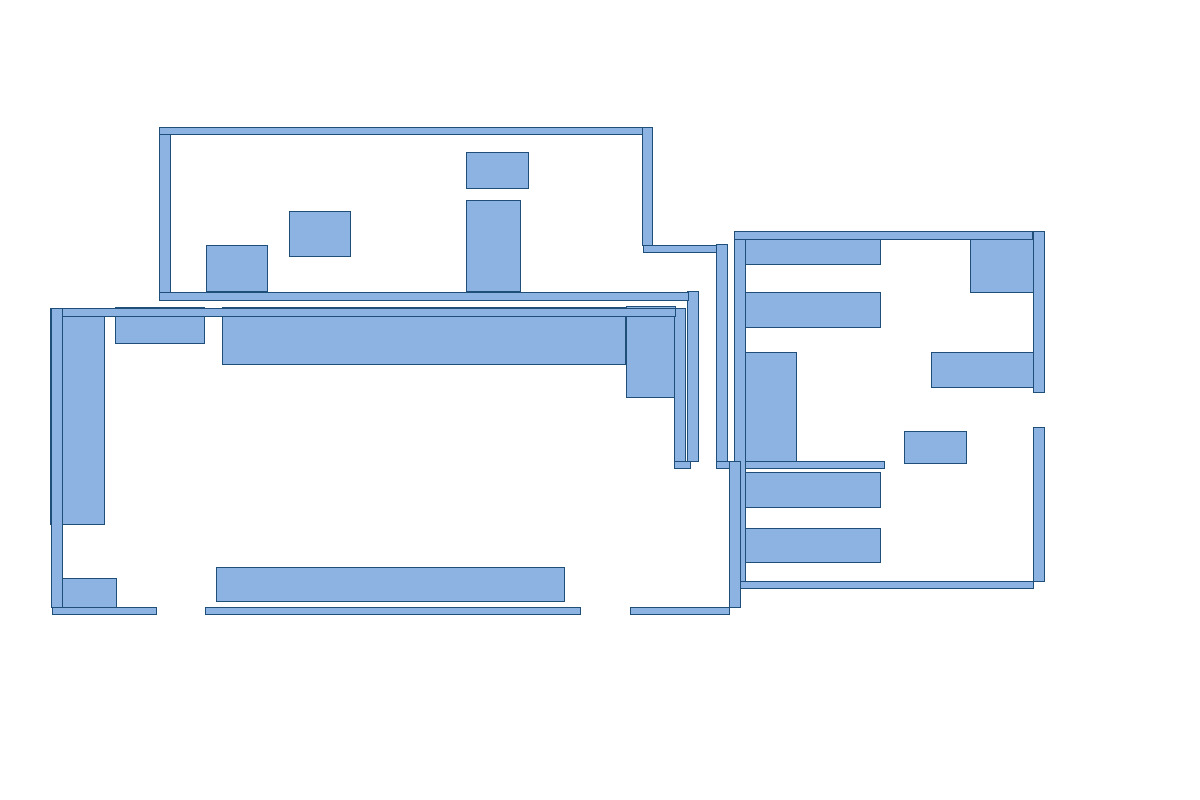
\includegraphics[width=.95\linewidth]{plan_overlay.png}
  \caption{Overlay technique généré à partir des obstacles normalisés.}
  \label{fig:a2-overlay}
\end{figure}

\subsection{Plan illustratif de l'aéroport (JPEG)}
Le fond illustratif utilisé pour les démonstrations (plan d’orientation de l’aéroport) est fourni pour référence.

\begin{figure}[h]
  \centering
  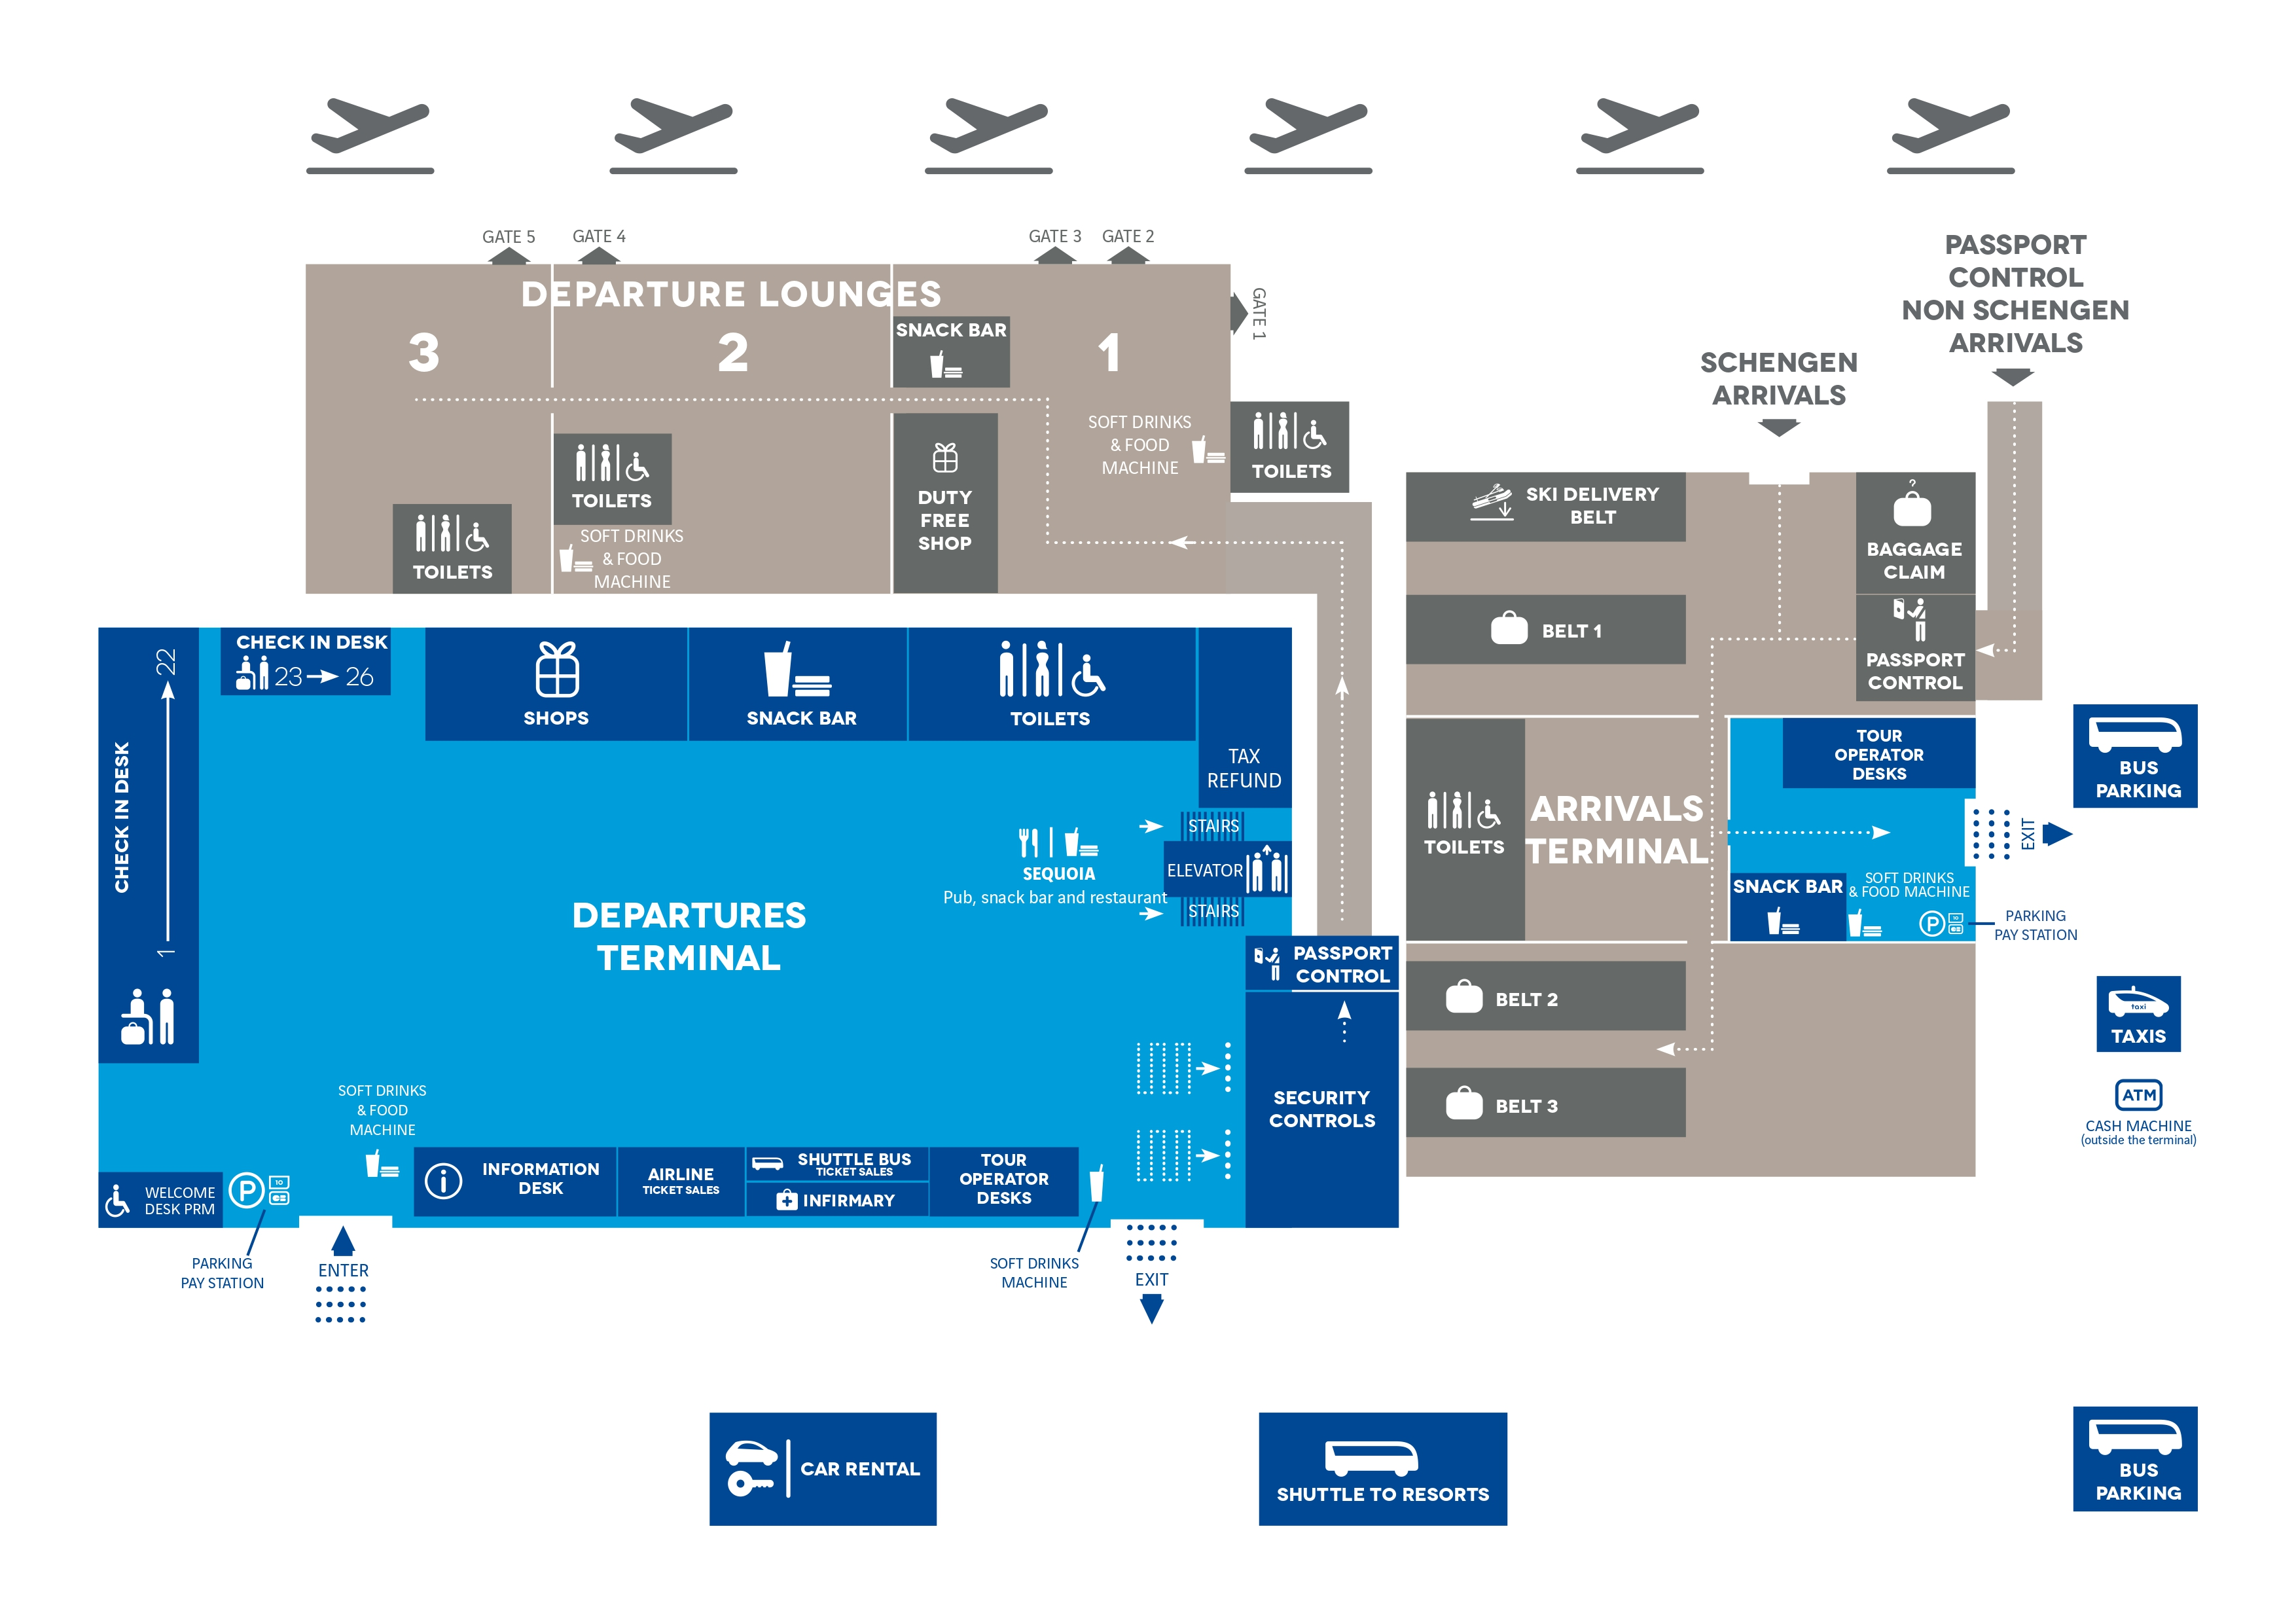
\includegraphics[width=.95\linewidth]{plan_interieur_gnb_hd.jpg}
  \caption{Plan illustratif de l'aéroport}
  \label{fig:a2-plan-jpeg}
\end{figure}

% =============================================================
% Annexe A3 — Tests et conformité (v4 — revue experte)
% -------------------------------------------------------------
\section{Tests et conformité}
\label{ann:a3-tests}

\subsection{Environnement et périmètre}
Après importation des fichiers, les tests techniques ont été réalisés sur Power~BI Desktop 
(canal classique) sous Windows~11, machine AMD Ryzen~7~9800X3D, 32~Go RAM, NVIDIA RTX~5080. 
Visuels évalués : \textit{Passenger-Flow Map} et \textit{Radial Sunburst Decomposition Tree} (version 2.0.0.0). 
Tailles mesurées des paquets \texttt{.pbiviz} (\textit{release} minifiée) : 
\textit{Radial Sunburst Decomposition Tree} \SI{37}{\kibi\byte} (\(\approx\) 37\,888~octets) ; 
\textit{Passenger-Flow Map} \SI{1006}{\kibi\byte} (\(\approx\) \SI{0.982}{\mebi\byte}). 
(Conversion effectuée depuis les valeurs «~Ko~» affichées par l’explorateur Windows vers KiB/MiB, norme IEC.) 
Jeux de données par défaut utilisés : \texttt{airport-flows-direct} et \texttt{sampleBudget}. 
Date des mesures : 05/08/2025 (cf. planning Waterfall du Chap.~3).

\begin{figure}[h]
  \centering
  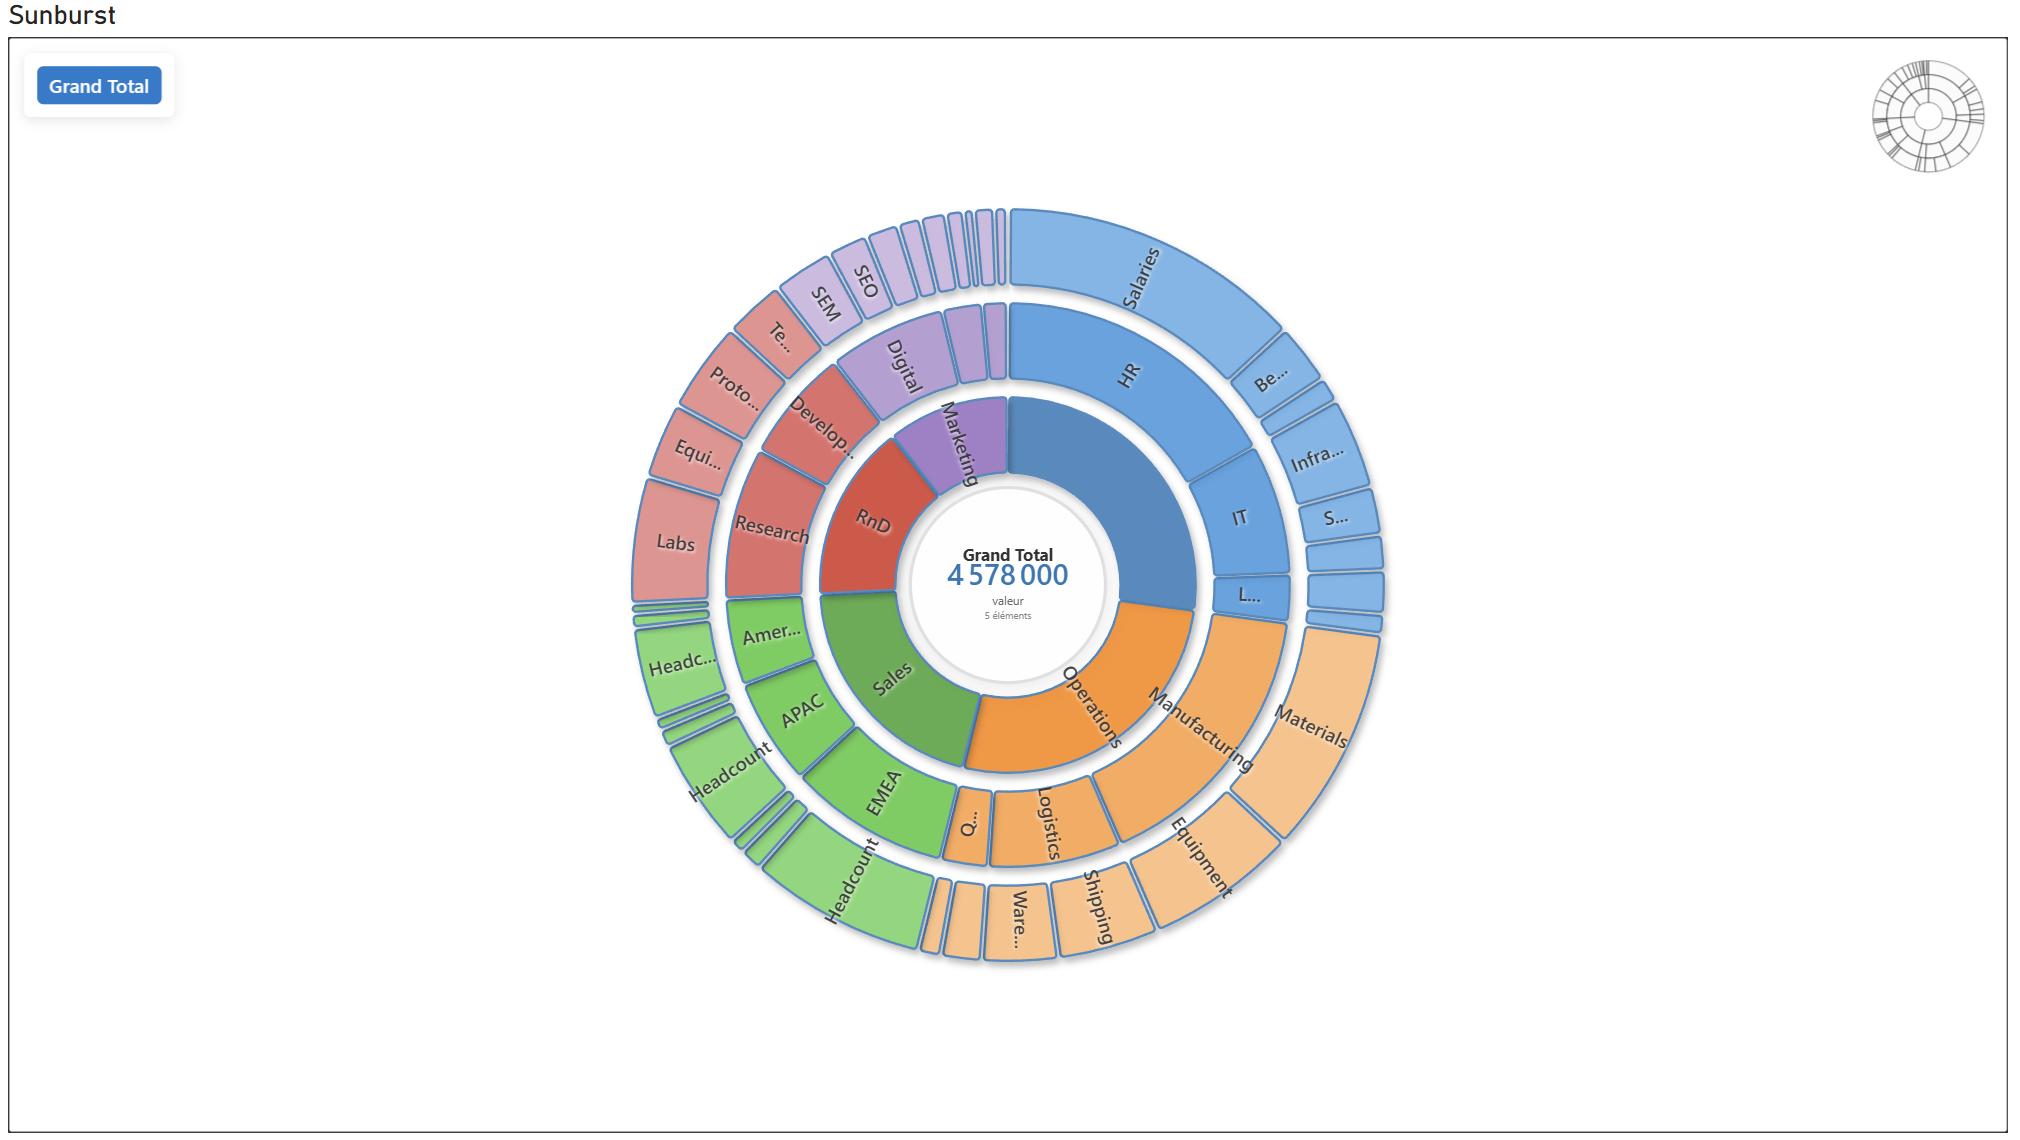
\includegraphics[width=.95\linewidth]{Sunburst.png}
  \caption{Radial Sunburst Decomposition Tree — rendu sur dataset budgétaire de démonstration.}
\end{figure}

\begin{figure}[h]
  \centering
  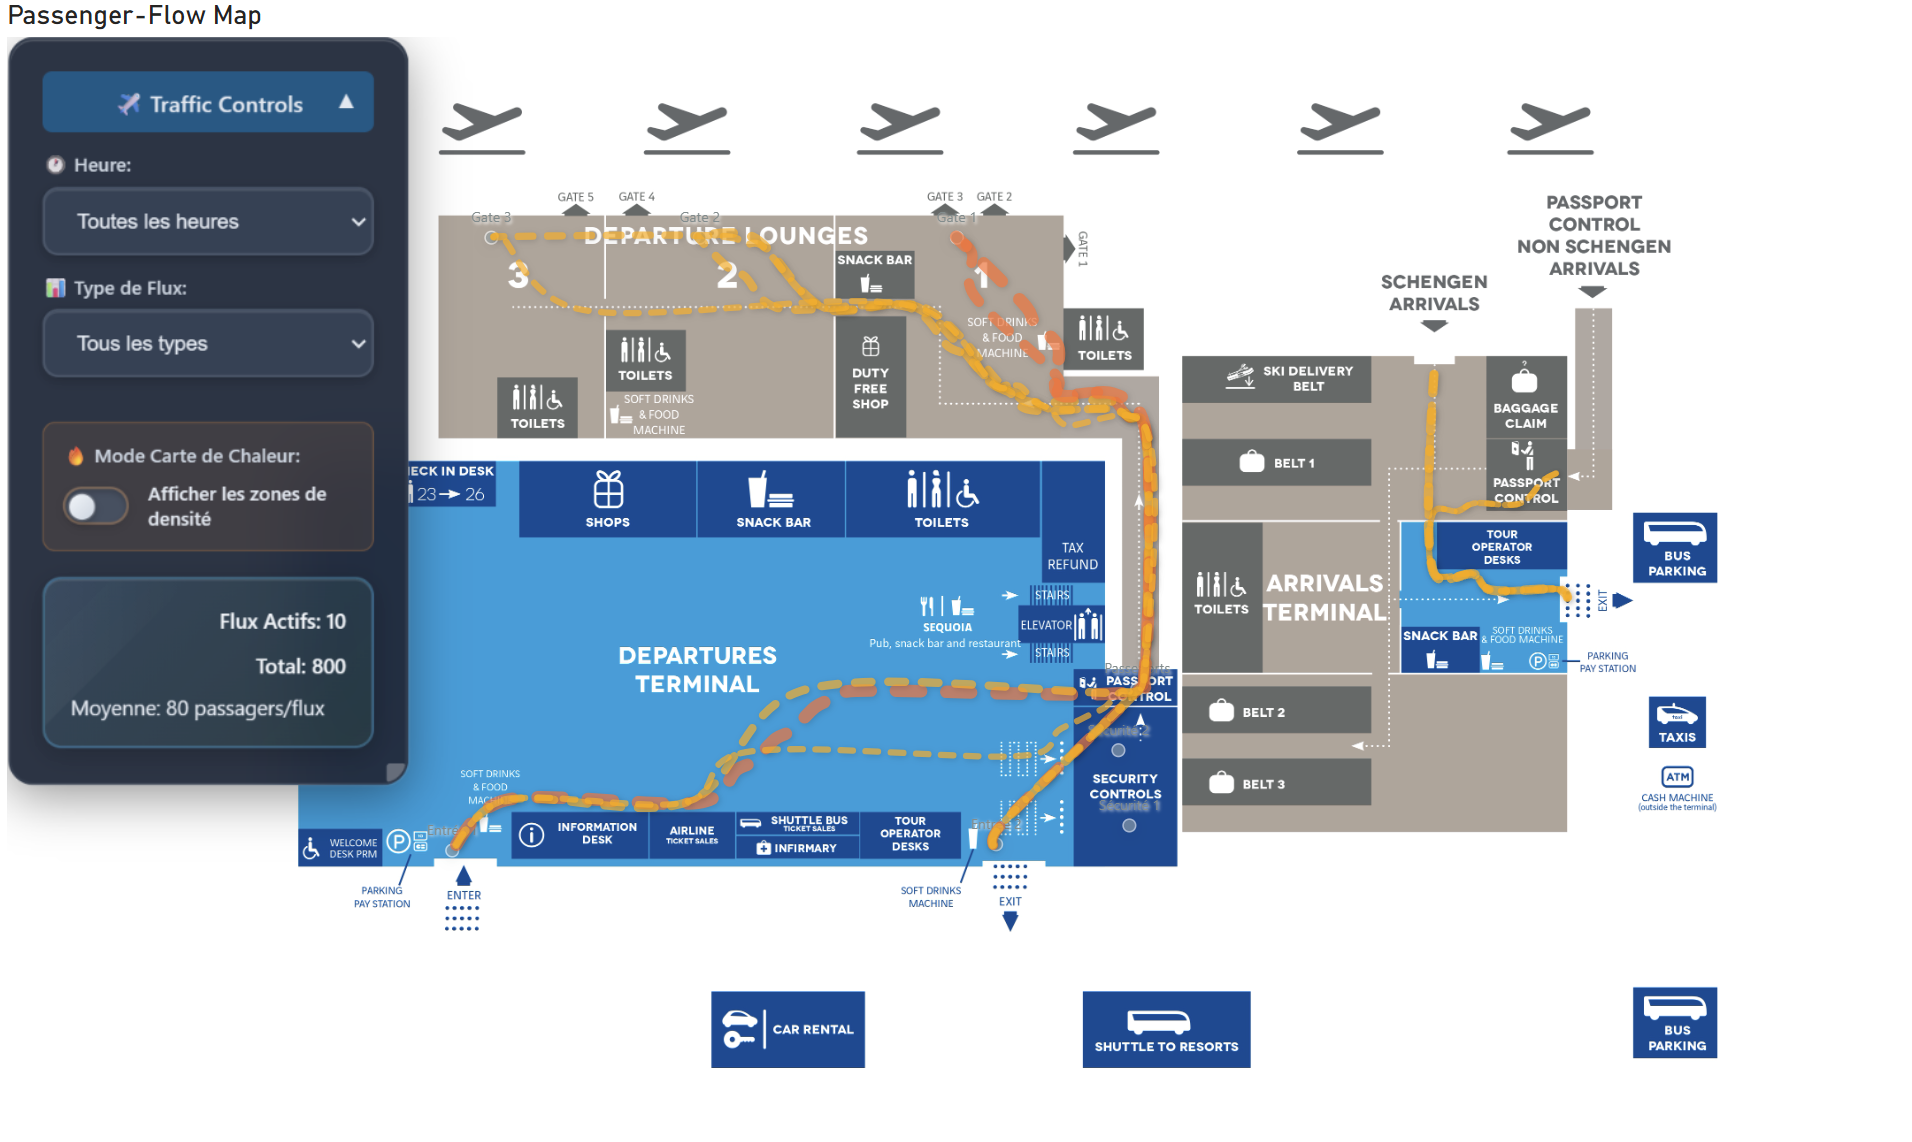
\includegraphics[width=.95\linewidth]{Passenger-flow.png}
  \caption{Passenger-Flow Map — rendu sur dataset de flux passagers de démonstration.}
\end{figure}

\subsection{Protocole de mesure}
Les mesures de performance ont été saisies depuis l’Analyseur de performances de Power~BI, 
en relevant la durée «~Visual display (ms)~».  
\textbf{Critères projet (P95)} : \textit{Passenger-Flow Map} \(\leq\) 300~ms ; 
\textit{Radial Sunburst Decomposition Tree} \(\leq\) 100~ms (par interaction : chargement, drill, survol).

En complément des mesures techniques, une \textbf{revue experte formative} a été menée par la professeure référente 
(cf. Chap.~\ref{sec:validation-fonctionnelle}) afin d’évaluer la lisibilité, l’ergonomie de base et l’adéquation fonctionnelle.  
Cette revue constitue la seule source de retours qualitatifs ; aucun test utilisateur ou démonstration interne n’a été conduit.

\subsection{Résultats (synthèse)}
\begin{table}[h]
\scriptsize
\setlength{\tabcolsep}{3pt}
\centering
\begin{tabularx}{\linewidth}{l l r r r r c}
\toprule
\textbf{Visuel} & \textbf{Scénario} & \textbf{$n$} & \textbf{Moy (ms)} & \textbf{P95 (ms)} & \textbf{Seuil P95 (ms)} & \textbf{Conforme ?} \\
\midrule
Radial Sunburst Decomposition Tree & Global & 20 & 38.0 & 46.1 & 100 & Oui \\
Passenger-Flow Map & Global & 19 & 131.1 & 167.9 & 300 & Oui \\
\bottomrule
\end{tabularx}
\end{table}

\subsection{Distribution des temps (visualisations)}
\begin{figure}[h]
  \centering
  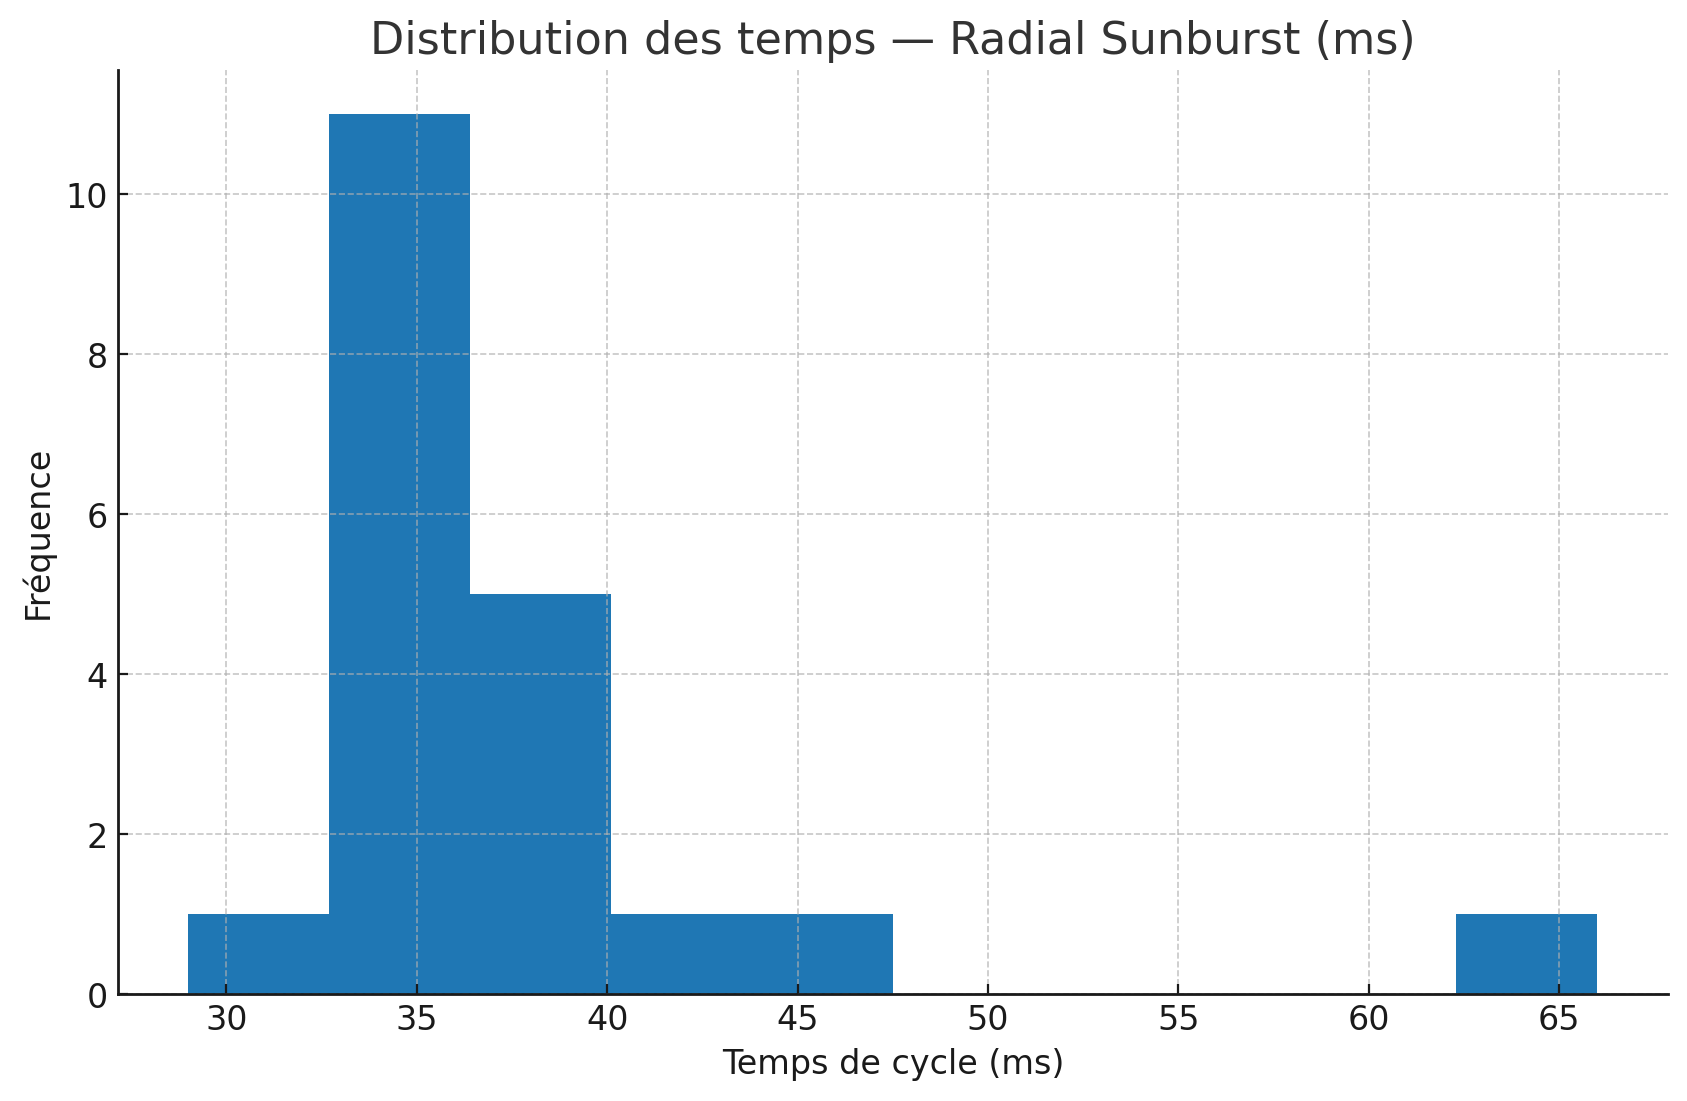
\includegraphics[width=.82\linewidth]{a4_sunburst_hist_v4.png}
  \caption{Radial Sunburst Decomposition Tree — histogramme des temps de cycle (ms).}
\end{figure}

\begin{figure}[h]
  \centering
  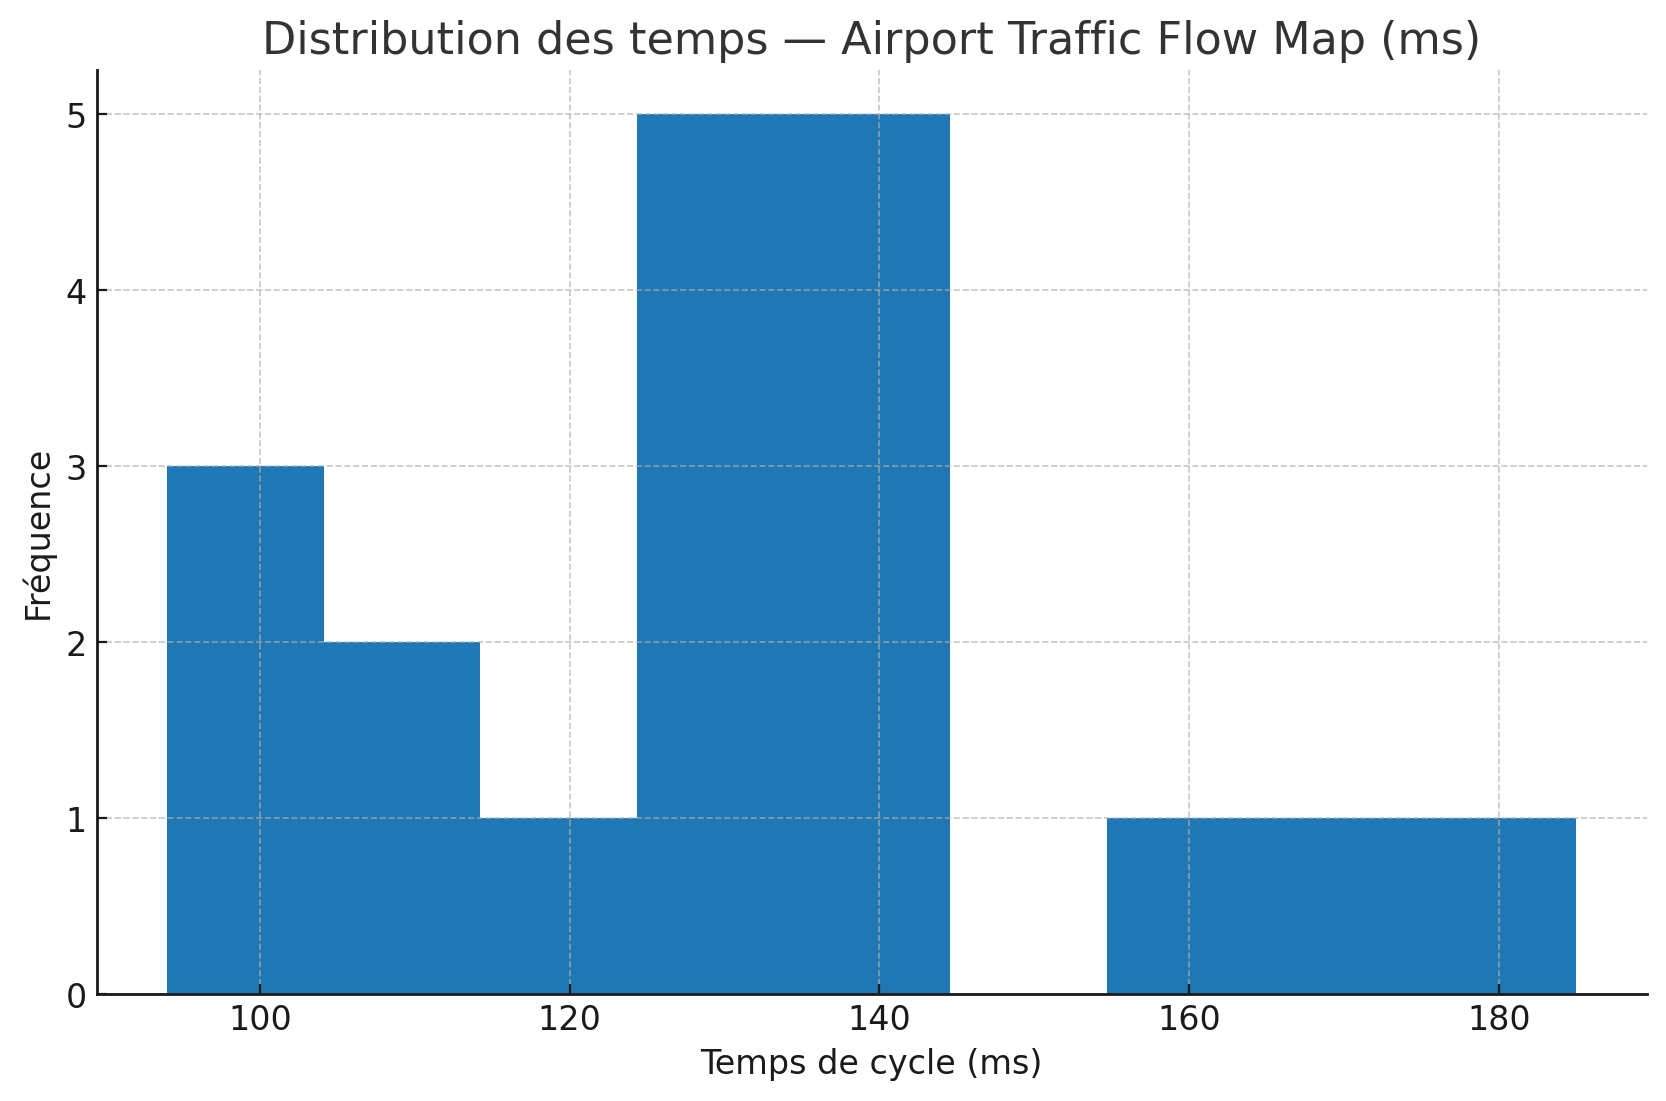
\includegraphics[width=.82\linewidth]{a4_map_hist_v4.png}
  \caption{Passenger-Flow Map — histogramme des temps de cycle (ms).}
\end{figure}

\subsection{Accessibilité (WCAG 2.2 — périmètre du projet)}
\begin{tabularx}{\linewidth}{l c X}
\toprule
\textbf{Critère} & \textbf{Statut} & \textbf{Preuve / commentaires} \\
\midrule
Navigation clavier (2.1.1) & Partiel & Non démontrable à partir des traces ; interactions testées principalement à la souris. À revérifier avec protocole clavier dédié. \\
Contraste (1.4.3) & À vérifier & Palette par défaut à contraste renforcé ; ratio à mesurer formellement sur les couples de couleurs configurés. \\
Internationalisation (3.1.x) & Conforme & Libellés fr-CH et en-US fournis ; bascule validée sur libellés de base. \\
\bottomrule
\end{tabularx}

\subsection{Sécurité et packaging}
\begin{tabularx}{\linewidth}{l X}
\toprule
\textbf{Vérification} & \textbf{État} \\
\midrule
Appels réseau sortants & Non utilisés (visuels autonomes, données locales Power BI). \\
\texttt{eval} / code dynamique & Non utilisé. \\
Stockage navigateur persistant & Non utilisé par défaut. \\
Taille du paquet \texttt{.pbiviz} & \textit{Radial Sunburst Decomposition Tree} \SI{37}{\kibi\byte} ; \textit{Passenger-Flow Map} \SI{1006}{\kibi\byte} (\(\approx\) \SI{0.982}{\mebi\byte}). \\
Seuil CI (artefact \texttt{.pbiviz}) & \(\leq\) \SI{1}{\mebi\byte} (= 1\,048\,576~octets). \\
Audit \texttt{--certification-audit} & À exécuter pour livraison : aucun blocant attendu sur ce périmètre. \\
\bottomrule
\end{tabularx}

\subsection{Couverture des tests unitaires}
\label{ann:a3-tests-coverage}

Les tests unitaires ont été exécutés avec Jest/ts-jest via \texttt{npm run test:cov} ; 
les rapports sont archivés dans \texttt{coverage/}.  
Le seuil CI retenu pour la couverture (déclarations) est fixé à \(\geq 70\%\). 
Les deux visuels satisfont ce seuil.

\begin{table}[H]\centering\small
\caption{Synthèse de couverture et d'exécution des tests}
\begin{tabular}{lrrrrrr}
\toprule
Visuel & \% Stmts & \% Branch & \% Funcs & \% Lines & Suites (ok/total) & Tests (ok/total) \\
\midrule
Radial Sunburst Decomposition Tree & 87.39 & 70.27 & 93.02 & 87.99 & 8/8  & 40/40 \\
Passenger-Flow Map                 & 80.64 & 76.30 & 75.45 & 80.66 & 19/19 & 51/51 \\
\bottomrule
\end{tabular}
\end{table}

En lecture rapide, le \textit{Sunburst} présente une couverture globalement élevée et homogène ; 
le \textit{Passenger-Flow Map} atteint des niveaux satisfaisants compte tenu de la part de logique graphique et d’interface.  
Ces résultats valident la robustesse des tests et la conformité au seuil CI sur le périmètre technique défini.

\section{Retours qualitatifs (revue experte)}
\label{ann:a4-retours}

Cette annexe synthétise les observations formulées lors de la revue experte réalisée 
par la professeure référente, en environnement Power~BI Service, 
sur les jeux de données de démonstration (\texttt{airport-flows-direct} et \texttt{sampleBudget}). 
Aucune autre session de test utilisateur ni démonstration interne n’a été conduite.

\subsection{Passenger-Flow Map}
\begin{itemize}[nosep]
  \item \textbf{Lisibilité des flux principaux} : claire dès le premier coup d’œil. Suggestion d’ajouter une variation d’épaisseur des traits par zone pour renforcer la hiérarchie visuelle.
  \item \textbf{Carte de chaleur} : pertinente pour repérer les zones d’affluence, mais l’échantillon de données de démonstration ne permet pas de tester pleinement son potentiel.
  \item \textbf{Légende et couleurs} : ajout d’une légende jugé utile ; possibilité de définir manuellement les paliers de couleur recommandée.
\end{itemize}

\subsection{Sunburst hiérarchique}
\begin{itemize}[nosep]
  \item \textbf{Hiérarchie et proportions} : compréhension immédiate.
  \item \textbf{Navigation} : drill-down, drill-up et fil d’Ariane jugés naturels et faciles à utiliser.
  \item \textbf{KPI central} : non indispensable mais pas gênant ; peut rester optionnel.
\end{itemize}

\subsection{Synthèse}
La revue experte conclut que les deux visuels répondent à leurs objectifs métier initiaux.  
La \textit{Passenger-Flow Map} apparaît comme un composant spécialisé, 
avec des pistes d’amélioration sur la personnalisation visuelle et la clarté des légendes.  
Le \textit{Sunburst} se distingue par sa polyvalence et son adaptabilité à différents contextes hiérarchiques.



\section{Procédure développeur}
\label{ann:a5-dev}

\subsection{Prérequis (environnement)}
\begin{tabularx}{\linewidth}{l X}
\toprule
\textbf{Composant} & \textbf{Version / Remarque} \\
\midrule
OS & Windows 11 (64-bit) \\
Power BI Desktop & Canal classique (build courant) \\
Node.js & 22.x (LTS) \\
npm & 10/11 \\
Power BI Visual Tools (pbiviz) & 6.1.3 \\
\bottomrule
\end{tabularx}

\subsection{Arborescence de référence}
\begin{lstlisting}[basicstyle=\ttfamily\small]
/ (racine du dépot)
  src/                  # sources TypeScript du visuel
  assets/               # ressources statiques (icones, styles)
  tests/                # tests unitaires Jest (optionnel)
  dist/                 # artefacts .pbiviz (généré)
  coverage/             # rapports de couverture (généré)
  scripts/              # scripts internes (signature, etc.)
    make_signing_keys.ps1
    make_signing_keys.sh
    openssl.cnf         # config locale si nécessaire (Windows)
  capabilities.json
  pbiviz.json
  package.json
  tsconfig.json
  .eslintrc.cjs
  .gitignore
\end{lstlisting}

\subsection{\texttt{tsconfig.json} (inclure les \texttt{.d.ts})}
\begin{lstlisting}[language=json,basicstyle=\ttfamily\small,breaklines=true,columns=fullflexible]
{
  "compilerOptions": {
    "allowJs": false,
    "emitDecoratorMetadata": true,
    "experimentalDecorators": true,
    "target": "es2022",
    "sourceMap": true,
    "outDir": "./.tmp/build/",
    "moduleResolution": "node",
    "declaration": true,
    "lib": ["es2022", "dom"]
  },
  "files": ["./src/visual.ts"],
  "include": ["src/**/*.ts", "src/**/*.tsx", "src/**/*.d.ts"],
  "exclude": ["node_modules", "dist", ".tmp", "coverage"]
}
\end{lstlisting}

\subsection{Scripts NPM (référence)}
\begin{lstlisting}[language=json,basicstyle=\ttfamily\small,breaklines=true,columns=fullflexible]
{
  "scripts": {
    "lint": "eslint . --ext .ts,.tsx -f stylish",
    "lint:ci": "eslint . --ext .ts,.tsx -f unix --max-warnings=0",
    "test": "jest --ci",
    "test:cov": "jest --ci --coverage --passWithNoTests --coverageReporters=json-summary --coverageReporters=text --coverageReporters=lcov",
    "start": "pbiviz start",
    "build": "pbiviz package"
  }
}
\end{lstlisting}

\subsection{Toolchain de build (devDependencies minimales)}
\begin{itemize}
  \item \texttt{webpack}, \texttt{webpack-cli}, \texttt{typescript}, \texttt{ts-loader}
  \item \texttt{css-loader}, \texttt{json-loader}, \texttt{less}, \texttt{less-loader}
  \item Qualité/tests : \texttt{eslint}, \texttt{@typescript-eslint/\{parser,eslint-plugin\}}, \texttt{jest}, \texttt{ts-jest}
\end{itemize}

\subsection{\texttt{.gitignore} (extraits pertinents)}
\begin{lstlisting}[basicstyle=\ttfamily\small]
node_modules/
dist/
coverage/
.tmp/
webpack.statistics*.html

# Clés/certificats internes (ne pas versionner)
scripts/ecrins-root.key
scripts/ecrins-root.crt
scripts/_codesign.key
scripts/_codesign.crt
*.p7s
\end{lstlisting}

\subsection{Démarrage local (dev)}
1) \texttt{npm ci}. 2) \texttt{pbiviz start}. Au premier lancement, installer le certificat HTTPS proposé par \texttt{pbiviz} (magasin « Autorités de certification racines de confiance »). 3) Power BI Desktop~\(\rightarrow\) Options~\(\rightarrow\) Sécurité~: activer le mode développeur. Le visuel Developer apparaît dans le ruban.

\subsection{Packaging local (\texttt{.pbiviz})}
Exécuter \texttt{pbiviz package --certification-audit}. Conserver le \texttt{packaging.log}. Vérifier l’incrément de version dans \texttt{pbiviz.json} (\(MAJOR.MINOR.PATCH\)). La CI orchestre les mêmes commandes (chap.~\ref{chap:industrialisation}).

\subsection{Contrôles rapides (QA)}
Lint \& tests~: \texttt{npm run lint} \& \texttt{npm test} ; taille du paquet \(\leq\)~1~MiB ; audit sans bloquant ; démarrage Desktop OK.
\section{Publication dans le magasin organisationnel : vérifications préalables et mode opératoire}
\label{ann:org-store-procedure}

\subsection{Pré-requis côté administrateur (mise à jour)}
Dossier attendu pour la revue :
\begin{itemize}
  \item Paquet \texttt{.pbiviz}
  \item Empreinte \texttt{.pbiviz.sha256}
  \item Journal d’audit (\texttt{packaging.log})
  \item Signature \texttt{.pbiviz.p7s} (si signature interne activée)
  \item Référence de version (tag Git) et changelog
  \item Certificat racine interne (\texttt{scripts/ecrins-root.crt}) pour vérification locale
\end{itemize}

\subsection{Vérification d’intégrité (SHA-256)}
\textbf{Linux/macOS}
\begin{verbatim}
sha256sum -c MonVisuel.pbiviz.sha256
# "OK" confirme la correspondance empreinte/fichier
\end{verbatim}
\textbf{Windows PowerShell}
\begin{verbatim}
Get-FileHash .\MonVisuel.pbiviz -Algorithm SHA256
# Comparer au contenu de MonVisuel.pbiviz.sha256
\end{verbatim}

\subsection{Vérification de la signature (si activée)}
\textbf{Linux/macOS}
\begin{verbatim}
openssl smime -verify -binary \
  -in MonVisuel.pbiviz.p7s -inform DER \
  -content MonVisuel.pbiviz \
  -CAfile scripts/ecrins-root.crt -purpose any -out /dev/null
# Code retour 0 : signature valide et chaîne approuvée
\end{verbatim}
\textbf{Windows}
Utiliser OpenSSL pour Windows avec la commande ci-dessus, ou importer la racine interne
dans le magasin d’autorités approuvées et utiliser l’outil interne.
% =============================================================
% A.6 — Activer la signature interne (parcours simple)
% =============================================================
\section{Activer la signature interne (parcours simple)}
\label{ann:signature-procedure}

\subsection*{Objet et périmètre}
Mise en place simple d’une signature interne pour les paquets \texttt{.pbiviz}. Optionnelle : sans activation, la vérification se limite à l’empreinte d’intégrité (SHA-256).

\subsection*{Étape 0 — Prérequis}
Installer OpenSSL.\\
\textbf{Windows (winget)} : \verb|winget install -e --id ShiningLight.OpenSSL.Light|\\
\textbf{macOS} : \verb|brew install openssl| \quad \\
\textbf{Linux (Debian/Ubuntu)} : \verb|sudo apt update && sudo apt install -y openssl|

\noindent\textit{Note (Windows).} Certaines distributions OpenSSL référencent un \texttt{OPENSSLDIR} non présent localement. Pour éviter les erreurs, fournir un fichier local \texttt{scripts/openssl.cnf} et, si nécessaire, le référencer via \texttt{-config}.

\begin{lstlisting}[basicstyle=\ttfamily\small]
openssl_conf = openssl_init
[openssl_init]
providers = provider_sect
[provider_sect]
default = default_sect
[default_sect]
activate = 1
[req]
distinguished_name = dn
[dn]
\end{lstlisting}

\subsection*{Étape 1 — Générer la racine et le certificat (scripts locaux)}
Créer \texttt{scripts/make\_signing\_keys.ps1} (Windows) ou \texttt{scripts/make\_signing\_keys.sh} (macOS/Linux), puis exécuter. Fichiers produits : \texttt{scripts/ecrins-root.crt},\\\texttt{scripts/ecrins-root.key}, \\\texttt{scripts/ecrins-codesign.crt}, \texttt{scripts/ecrins-codesign.key}. Une passphrase est affichée ; la conserver en lieu sûr.

\textbf{PowerShell (Windows) — \texttt{scripts/make\_signing\_keys.ps1}}
\begin{lstlisting}[basicstyle=\ttfamily\small,breaklines=true,columns=fullflexible]
param(
  [string]$Country="CH", [string]$Org="ECRINS SA",
  [string]$RootCN="ECRINS Visuals Root CA",
  [string]$CodeCN="ECRINS Visuals Code Signing",
  [int]$RootDays=3650, [int]$CodeDays=1095
)
$ErrorActionPreference = "Stop"
function New-RandBase64([int]$n=32){
  $b=New-Object byte[] $n
  [Security.Cryptography.RandomNumberGenerator]::Create().GetBytes($b)
  [Convert]::ToBase64String($b)
}
if(-not(Get-Command openssl -ErrorAction SilentlyContinue)){
  Write-Error "OpenSSL indisponible"
}
New-Item -ItemType Directory -Force -Path "scripts" | Out-Null
Push-Location scripts
@"
openssl_conf = openssl_init
[openssl_init]
providers = provider_sect
[provider_sect]
default = default_sect
[default_sect]
activate = 1
[req]
distinguished_name = dn
[dn]
"@ | Set-Content -Encoding ascii openssl.cnf
$config = (Resolve-Path .\openssl.cnf).Path
$rootPass=New-RandBase64; $codePass=New-RandBase64
# Racine
openssl genpkey -algorithm RSA -out ecrins-root.key -aes-256-cbc -pass pass:$rootPass -pkeyopt rsa_keygen_bits:4096
openssl req -x509 -new -key ecrins-root.key -passin pass:$rootPass -sha256 -days $RootDays -subj "/C=$Country/O=$Org/CN=$RootCN" -config "$config" -out ecrins-root.crt
# Signature
openssl genpkey -algorithm RSA -out ecrins-codesign.key -aes-256-cbc -pass pass:$codePass -pkeyopt rsa_keygen_bits:3072
openssl req -new -key ecrins-codesign.key -passin pass:$codePass -subj "/C=$Country/O=$Org/CN=$CodeCN" -config "$config" -out ecrins-codesign.csr
@"
basicConstraints=CA:FALSE
keyUsage=digitalSignature
extendedKeyUsage=codeSigning
subjectKeyIdentifier=hash
authorityKeyIdentifier=keyid,issuer
"@ | Set-Content -Encoding ascii codesign.ext
openssl x509 -req -in ecrins-codesign.csr -CA ecrins-root.crt -CAkey ecrins-root.key -passin pass:$rootPass -CAcreateserial -out ecrins-codesign.crt -days $CodeDays -sha256 -extfile codesign.ext
Write-Host "`nSecrets à créer : ECRINS_CODESIGN_CRT / ECRINS_CODESIGN_KEY / ECRINS_CODESIGN_PASS"
Write-Host ("ECRINS_CODESIGN_PASS = {0}" -f $codePass)
Pop-Location
\end{lstlisting}

\textbf{Bash (macOS/Linux) — \texttt{scripts/make\_signing\_keys.sh}}
\begin{lstlisting}[basicstyle=\ttfamily\small,breaklines=true,columns=fullflexible]
#!/usr/bin/env bash
set -euo pipefail
C="${1:-CH}"; O="${2:-ECRINS SA}"
ROOT_CN="${3:-ECRINS Visuals Root CA}"
CODE_CN="${4:-ECRINS Visuals Code Signing}"
ROOT_DAYS="${5:-3650}"; CODE_DAYS="${6:-1095}"
mkdir -p scripts && cd scripts
code_pass="$(openssl rand -base64 32)"
root_pass="$(openssl rand -base64 32)"
cat > openssl.cnf <<'CNF'
openssl_conf = openssl_init
[openssl_init]
providers = provider_sect
[provider_sect]
default = default_sect
[default_sect]
activate = 1
[req]
distinguished_name = dn
[dn]
CNF
# Racine
openssl genpkey -algorithm RSA -out ecrins-root.key -aes-256-cbc -pass pass:"$root_pass" -pkeyopt rsa_keygen_bits:4096
openssl req -x509 -new -key ecrins-root.key -passin pass:"$root_pass" -sha256 -days "$ROOT_DAYS" -subj "/C=$C/O=$O/CN=$ROOT_CN" -config openssl.cnf -out ecrins-root.crt
# Signature
openssl genpkey -algorithm RSA -out ecrins-codesign.key -aes-256-cbc -pass pass:"$code_pass" -pkeyopt rsa_keygen_bits:3072
openssl req -new -key ecrins-codesign.key -passin pass:"$code_pass" -subj "/C=$C/O=$O/CN=$CODE_CN" -config openssl.cnf -out ecrins-codesign.csr
cat > codesign.ext <<'EOF'
basicConstraints=CA:FALSE
keyUsage=digitalSignature
extendedKeyUsage=codeSigning
subjectKeyIdentifier=hash
authorityKeyIdentifier=keyid,issuer
EOF
openssl x509 -req -in ecrins-codesign.csr -CA ecrins-root.crt -CAkey ecrins-root.key -passin pass:"$root_pass" -CAcreateserial -out ecrins-codesign.crt -days "$CODE_DAYS" -sha256 -extfile codesign.ext
echo "ECRINS_CODESIGN_PASS = $code_pass"
\end{lstlisting}

\noindent\textbf{Exécution.}
\begin{verbatim}
# Windows
pwsh -File scripts/make_signing_keys.ps1

# macOS/Linux
chmod +x scripts/make_signing_keys.sh
./scripts/make_signing_keys.sh
\end{verbatim}

\subsection*{Étape 2 — Créer les secrets GitHub (noms exacts)}
Dans \textit{Settings} → \textit{Secrets and variables} → \textit{Actions} → \textit{New repository secret}.\\
\texttt{ECRINS\_CODESIGN\_CRT} → contenu de \texttt{scripts/ecrins-codesign.crt}\\
\texttt{ECRINS\_CODESIGN\_KEY} → contenu de \texttt{scripts/ecrins-codesign.key}\\
\texttt{ECRINS\_CODESIGN\_PASS} → passphrase affichée

\subsection*{Étape 3 — Lancer une release}
Créer un tag \texttt{vX.Y.Z} et le pousser. La CI publie : \texttt{.pbiviz}, \texttt{.pbiviz.sha256}, \texttt{packaging.log} et, si secrets présents, \texttt{.pbiviz.p7s}. Voir l’annexe~\ref{ann:org-store-procedure} pour la vérification d’intégrité et de signature.

\subsection*{Sécurité}
Ne pas versionner \texttt{scripts/ecrins-root.key} ni \texttt{scripts/ecrins-root.crt}. Restreindre l’accès aux secrets GitHub et planifier leur rotation.



% -----------------------------------------------------------------------------
% Back matter
% -----------------------------------------------------------------------------
\backmatter

% Bibliography
\clearpage
\printbibliography[title={Références}, heading=bibintoc]

% Ensure your .bib file does not contain invalid characters in the 'howpublished' field.
% If the issue persists, try using a different bibliography style or remove problematic entries.

\clearpage
% Glossary
\printglossaries

% Page for student info and signatures
%\cleardoublepage
\chapter*{Informations sur ce travail}

\vspace{\fill}

\textbf{Informations de contact}

\begin{tabularx}{\textwidth}{N{2.5cm}X}
	Auteur:	& \AuthorFirstName \space \AuthorLastName \\
	& HES-SO Valais-Wallis \\
	E-mail: & \email{\AuthorEmail}
\end{tabularx}

\vspace{8.5cm}

\textbf{Déclaration sur l’honneur}

{\renewcommand{\arraystretch}{2}
\begin{tabularx}{\textwidth}{N{2.5cm}X}
	& Je déclare, par ce document, que j'ai effectué le travail 
	  de bachelor ci-annexé seul, sans autre aide que celles dûment 
	  signalées dans les références, et que je n'ai utilisé que les 
	  sources expressément mentionnées. Je ne donnerai aucune copie de 
	  ce rapport à un tiers sans l'autorisation conjointe du RF et du 
	  professeur chargé du suivi du travail de bachelor, à l'exception des 
	  personnes qui m'ont fourni les principales informations nécessaires 
	  à la rédaction de ce travail. \\
	Lieu, date: & \underline{\hspace{7cm}} \\ 
	Signature: & \underline{\hspace{7cm}}
\end{tabularx}
}

\vspace{\fill}

\end{document}
